%&pdflatex
\documentclass[a4paper,11pt,titlepage, article, oneside]{memoir}
%\semiisopage

\usepackage[margin=3cm]{geometry}
\usepackage[T1]{fontenc}
\usepackage[english]{babel}
% usare latin1 con windows
\usepackage[utf8]{inputenc}
% usare utf8 con linux
%\usepackage[uft8]{inputenc}
\usepackage{color, graphicx}%per scrivere con diversi colori
\usepackage{hyperref}
\usepackage{faktor}
\usepackage{hyperref}
\usepackage[makeroom]{cancel}
\usepackage{pgfplots}
\usepgfplotslibrary{patchplots}
\usetikzlibrary{patterns, positioning, arrows}
\pgfplotsset{compat=1.15}
\usepackage{float, subcaption, braket, bbold, amssymb,amsthm,amsmath,mathtools, tikz-cd}
\usepackage{stackengine}
\usepackage{fancyhdr}
\usepackage{musicography}
\usepackage[numbers]{natbib}
\defcitealias{Lee}{[Lee]}

\pagestyle{fancy}
\fancyhf{}
\fancyhead[L]{\rightmark}
\fancyhead[R]{\thepage}
\renewcommand{\headrulewidth}{0pt}



\usepackage{tcolorbox}
\tcbuselibrary{breakable}
\tcbset{breakable, colback=gray!8!white,colframe=gray!15!white}

\newtcolorbox{remarkbox}{breakable,   colback=white,colframe=gray}

\newtcolorbox{eqnbox}{colback=blue!5!white,colframe=blue!20!black, sharp corners}

\newcommand\crule[3][black]{\textcolor{#1}{\rule{#2}{#3}}}

%%% Definizione degli ambienti tipo "Teorema"
%\newtheorem{theorem}{Theorem}[chapter]

%\theoremstyle{theorem}
%\newtheorem{lemma}[theorem]{Lemma}
%\newtheorem{proposition}[theorem]{Proposition}
%\newtheorem{corollary}[theorem]{Corollary}
%\theoremstyle{definition}
%\newtheorem{definition}[theorem]{Definition}
%\theoremstyle{remark}
%\newtheorem{remark}[theorem]{Remark}
%\newtheorem{example}[theorem]{Example}

\numberwithin{equation}{section}
\counterwithout{section}{chapter}

\newtheorem{theorem}{Theorem}[section]
\newtheorem{corollary}[theorem]{Corollary}
\newtheorem{proposition}[theorem]{Proposition}
\newtheorem{lemma}[theorem]{Lemma}
\newtheorem{fact}[theorem]{Fact}

\theoremstyle{definition}
\newtheorem{definition}[theorem]{Definition}

\theoremstyle{remark}
\newtheorem{remark}[theorem]{Remark}
\newtheorem{example}[theorem]{Example}



% aumenta la spaziatura
\linespread{1.2}

\DeclareMathOperator{\id}{id}
\DeclareMathOperator{\Index}{Index}
\DeclareMathOperator{\rank}{rank}
\DeclareMathOperator{\tr}{tr}
\DeclareMathOperator{\pr}{pr}
\DeclareMathOperator{\Der}{Der}
\DeclareMathOperator{\Diff}{Diff}
\DeclareMathOperator{\sgn}{sgn}
\DeclareMathOperator{\supp}{supp}
\DeclareMathOperator{\im}{im}
% \DeclareMathOperator{i}{i}
\newcommand{\rfield}{\mathbb{R}}
\newcommand{\lie}[1]{\mathfrak{#1}}

%\renewenvironment{proof}[1][\proofname]{\textit{#1.}}{\qed}


\newcommand\oast{\stackMath\mathbin{\stackinset{c}{0ex}{c}{0ex}{\ast}{\bigcirc}}}

\newcommand\ocdot{\stackMath\mathbin{\stackinset{c}{0ex}{c}{0ex}{\cdot}{\bigcirc}}}

%\newcommand{\restrict}[2]{\left.{#1}\right|_{#2}}

\newcommand{\restrict}[2]{{#1}\raisebox{-.5ex}{$|$}_{#2}}

\newcommand{\diondi}[1]{\frac{d}{d{#1}}}

\newcommand{\difondi}[2]{\frac{d{#1}}{d{#2}}}

\newcommand{\deonde}[1]{\frac{\partial}{\partial {#1}}}

\newcommand{\defonde}[2]{\frac{\partial {#1}}{\partial {#2}}}

\newcommand{\tangentgeom}[1]{T_{#1}^{\text{geom}}}

\newcommand{\tangentphys}[1]{T_{#1}^{\text{phys}}}

\newcommand{\tangentalg}[1]{T_{#1}^{\text{alg}}}

\usetikzlibrary{calc}

\newcommand{\tikzmark}[1]{\tikz[overlay,remember picture] \node (#1) {};}
\newcommand{\DrawBox}[1][]{%
    \tikz[overlay,remember picture]{
    \draw[red,#1]
      ($(left)+(-0.2em,1.5em)$) rectangle
      ($(right)+(3em,-1.0em)$);}
}



\begin{document}
\pagenumbering{gobble}

\begin{tabular}[t]{r@{\hspace{0.5cm}}l}


	\parbox[b][5cm][t]{0.9\textwidth}{ 
\begin{flushright}

 {\Huge\bfseries\fontfamily{pnc}\selectfont Lecture Notes \\ \huge Differentiable Manifolds \\  \Large Ludwig-Maximilians-Universit\"at M\"unchen \\ Winter Semester 2019/2020 \\[\baselineskip]}
 % ----------------------------------------------------------------
 \vspace{15cm}
 %{\Large\bfseries }\\[5pt]
 
  \vfill
  {\large\fontfamily{pnc}\selectfont Flavio Rossetti}
  \end{flushright}
  }
  &
  \parbox[b][5cm][t]{1cm}{\rule{1pt}{\textheight}}
  
 \end{tabular}





\newpage
 {These notes are based on the content of the course \textit{Differentiable Manifolds} held at LMU during the Winter Semester 2019/2020. Some additional content from books and from my own studies was also added. These notes are neither complete nor accurate. They might contain typos and mistakes. You can send an email to \href{mailto:flaviorossetti@outlook.com}{\nolinkurl{flaviorossetti@outlook.com}} to help me improve these notes. Any help would be greatly appreciated!\\[13pt]}

 {These notes were compiled on \today. For the last version, check \url{https://github.com/fla-io/diff-manifolds}.}

  \vfill
  \vspace{1.5cm}
 %{\Large\bfseries }\\[5pt]
 \begin{center}
 \textit{Thanks to Janik Kruse and Ra\'ul Morral for their help to improve the script!}
 \end{center}

\newpage

\pagenumbering{Roman}
% indice

\tableofcontents
\clearpage

%%%%%%%%%%%%%%%%%%%%%%%%%%%%%%%%%%%%%%%%%%%%%%%%%%%%%%%%%%%%%%%%
\pagenumbering{arabic}

%\chapter{Part I}
\section[Introduction]{\crule[red!50!white]{0.3cm}{0.4cm}  Introduction}

From the Lee book \citetalias{Lee}: "The central idea of calculus is \textit{linear approximation}". A function of one variable can be approximated by its tangent line, a curve by a tangent vector (i.e. velocity vector), a surface in $\rfield^3$ can be approximated by its tangent plane, and a map from $\rfield^n$ to $\rfield^m$ by its total derivative.
Here it comes the importance of tangent spaces.

Main idea: in order to study tangent vectors, we identify them with "directional derivatives". In particular, there is a natural one-to-one correspondence between geometric tangent vectors and linear maps from $C^{\infty}(\rfield^n)$ to $\rfield$ satisfying the product rule. Such maps are called \textit{derivations}.


\begin{remarkbox}\begin{remark} \label{pointorvec}
\textbf{Points or vectors?} We can think of elements of $\rfield^n$ either as points or vectors. As points, their only property is their location, given by the coordinates $(x_1, \ldots, x_n)$ on a chosen basis. As vectors, they are characterized by a direction and a magnitude, but their location is irrelevant (translational invariance). So given $v \in \rfield^n, v=\sum_i v^i e_i = v^i e_i$, it can be seen as an arrow with its initial point anywhere in $\rfield^n$. So, if we think about a vector tangent to the border of the sphere at a point $a$, we imagine the vector as living in a copy of $\rfield^n$ with its origin translated to a.

\end{remark}\end{remarkbox}

\section[Notations and Conventions]{\crule[black!50!white]{0.3cm}{0.4cm}  Notations and Conventions}

In these notes the Einstein summation convention will be used. It means that the sum symbol will be omitted when it is clear with respect to which index we are summing. For instance we will write
$$v^i e_i$$
instead of
$$\sum\limits_i v^i e_i \, .$$
Given a map $f$ from a set $X$ to a set $Y$, we will denote it by
$$f \colon X \rightarrow Y \, .$$
We will use the arrow "$\mapsto$" to denote how each element of $X$ is mapped into $Y$ through $f$. For instance, given $x_1, x_2 \in X, y \in Y$, we will either use the notation:
$$x_1 \mapsto f(x_1)$$
or
$$x_2 \mapsto y \,.$$
We will use the symbol $\equiv$ in order to define mathematical objects.
We will use the latin abbreviation "i.e." (\textit{id est}) to explain concepts in a more detailed way, and the abbreviation "e.g." (\textit{exempli gratia}) to give examples.

\section[Quick review: Basic Algebraic Structures]{\crule[blue!50!white]{0.3cm}{0.4cm}  Quick review: Basic Algebraic Structures}

\begin{definition} [Operation]
Let $G$ be a set. The map:
\begin{align*}
\cdot \, \colon G &\times G \longrightarrow G \\
(&a, b) \longmapsto a \cdot b
\end{align*}
is called a (binary) operation on $G$.
Sometimes such a map is also denoted by the symbol $+$.
\end{definition}

\begin{definition} [Group] Given a set $G$ and an operation $\cdot$ on such set, we will call such set with the operation  (i.e. the couple $(G, \cdot)$) a group if the following properties are satisfied for all $a, b, c \in G$:
\begin{itemize}
\item $ a \cdot b \in G$,
\hspace*{\fill}\textit{(closure property)}
\item $a \cdot (b \cdot c) = (a \cdot b) \cdot c$,
\hspace*{\fill}\textit{(associativity)}
\item $\exists\, \mathbf{1} \in G$ such that $\mathbf{1} \cdot g = g, \, \forall\, g \in G$,
\hspace*{\fill}\textit{(existence of the identity element)}
\item $\forall\, g \in G, \exists\, g^{-1} \in G$ so that $g \cdot g^{-1} = g^{-1} \cdot g = \mathbf{1}$.
\hspace*{\fill} \textit{(existence of the inverse element)}
\end{itemize}
For the sake of simplicity, we will often call $G$ a group, without referring to the operation on it.
\end{definition}


\begin{tcolorbox}\begin{example}
$(\mathbb{Z}, +)$ is a group.
\end{example}\end{tcolorbox}

\begin{tcolorbox}\begin{example}
$(\mathbb{R}, +)$ is a group. Also: $(\mathbb{R} \setminus \{0\}, \cdot)$ is a group.
\end{example}\end{tcolorbox}

\begin{tcolorbox}\begin{example}
$(\mathbb{N}, +)$ is not a group!
\end{example}\end{tcolorbox}

\begin{remarkbox}\begin{remark} \label{zeroone}
The identity element of a group is often denoted as $\mathbf{1}$ if the operation is denoted by the symbol $\cdot$, whereas it is denoted as $\mathbf{0}$ if the operation is denoted by the symbol $+$.
In a similar way, the inverse element is often denoted as $g^{-1}$ if the operation is denoted by the symbol $\cdot$, whereas it is denoted as $-g$ if the operation is denoted by the symbol $+$.

\end{remark}\end{remarkbox}

\begin{definition} [Abelian group]
A group $(G, \cdot)$ is called abelian if its elements commute according to the operation $\cdot$, i.e. $a \cdot b = b \cdot a, \forall \,  a, b \in G$.
\end{definition}

Often we can consider sets with two operations, like $(\mathbb{R}, + , \cdot)$. If they satisfy some properties, they are called rings. If they satisfy even more properties, they are called fields. In particular:

\begin{definition} [Ring]
Given a set $R$ and two operations: $+$ (usually called "additive operation") and $\cdot$ (called "multiplicative operation") on it, we will call the set with the two operations, i.e. $(R, +, \cdot)$, a ring if the following properties are satisfied:
\begin{itemize}
\item $(R, +)$ is an abelian group,
\item $\cdot$ is associative, i.e. $a \cdot (b \cdot c) = (a \cdot b) \cdot c, \, \forall\, a, b, c, \in R$,
\item $\cdot$ is distributive with respect to $+$, i.e. $a \cdot (b + c) = a \cdot b + a \cdot c$ and $ (b + c) \cdot a = b \cdot a + c \cdot a$.
\end{itemize}
\end{definition}

\begin{definition} [Commutative ring] $(R, +, \cdot)$ is a commutative ring if the multiplication operation $\cdot$ is commutative.
\end{definition}

\begin{definition} [Unitary ring]
$(R, +, \cdot)$ is a unitary ring if it contains the multiplicative identity, i.e. $\exists\, \mathbf{1} \in R$ such that $\mathbf{1} \cdot r = r \cdot \mathbf{1} =  r, \, \forall\, r \in R$ .
\end{definition}

\begin{definition}[Invertible element]
An element $a$ in a ring $(R, +, \cdot)$ is called invertible if there exists its inverse according to the multiplicative operation, i.e. $\exists\, b \in R$ such that $a \cdot b = b \cdot a = \mathbf{1}$. We will also write $a^{-1} \equiv b$.
\end{definition}

\begin{definition} [Field]
A unitary, commutative ring such that every non-zero element is invertible is called a field.
\end{definition}

\begin{remarkbox}\begin{remark}
When we talk about the zero element in a field or in a ring we always refer to the identity element according to the additive operation. See also remark \ref{zeroone}.
\end{remark}\end{remarkbox}

\begin{tcolorbox}\begin{example}
The set of $2 \times 2$ matrices with real coefficients is a ring with the operations of sum between matrices and with the matrix multiplication. The ring is not commutative because the matrix multiplication is not a commutative operation. It is unitary, since the identity matrix is the multiplicative identity. But it's not a field because not every matrix is invertible (just take a matrix with zero determinant).
\end{example}\end{tcolorbox}

\begin{tcolorbox}\begin{example}
$(\mathbb{Z}, +, \cdot)$ is a unitary, commutative ring. It is not a field since the inverse element for $\cdot$ is often in the rational numbers, i.e. $3^{-1}$ is the multiplicative inverse of $3$.
\end{example}\end{tcolorbox}

\begin{tcolorbox}\begin{example}
$(\mathbb{R}, +, \cdot)$ is a field.
\end{example}\end{tcolorbox}

\section[Quick review: Morphisms]{\crule[blue!70!white]{0.3cm}{0.4cm}  Quick review: Morphisms}
\begin{definition}[Homomorphism]
A homomorphism $h$ between two sets endowed with structures (think about two groups, for instance) is a map which preserves the structure, i.e. a map
\begin{equation*}
h \colon (G, +) \longrightarrow (H, \circ)
\end{equation*}
such that $h(a + b) = h(a) \circ h(b), \forall\, a, b, \in G$, where $(G, +)$ and $(H, \circ)$ are two groups. The definition for rings and fields is analogous. People from category theory also tend to call (group) homomorphisms just (group) morphisms since the morphisms in the category \textbf{Grp} of all groups are set to be group homomorphisms.
\end{definition}

Now, we can consider some particular types of homomorphisms.

\begin{remarkbox}\begin{remark} [Monomorphism, epimorphisms and isomorphisms]
Homomorphisms can be called in different ways depending whether they are injective, surjective or bijective.
A monomorphism is an injective homomorphism. An epimorphism is a surjective homomorphism. An isomorphism is a bijective homomorphism (thus, it is both a monomorphism and an epimorphism).
\end{remark}\end{remarkbox}

\begin{remarkbox}\begin{remark} [Endomorphism, automorphism] \label{endoremark}
An endomorphism is a homomorphism from one algebraic structure to itself. If such a morphism is bijective, it is called automorphism.
\end{remark}\end{remarkbox}

\begin{remarkbox}\begin{remark} \label{homeoremark}
Don't get confused with hom\underline{e}omorphisms! A homeomorphism is a continuous and bijective map between two topological spaces, such that its inverse is also continuous. In general it is not a homomorphism (without the \textbf{e}).
\end{remark}\end{remarkbox}

\section[Quick review: Equivalence Classes, Quotient Spaces]{\crule[blue!90!white]{0.3cm}{0.4cm}  Quick review: Equivalence Classes, Quotient Spaces}
\begin{definition}[Binary relation]
  Given a set $E$, a (binary) relation $\sim$ on $E$ is a set of couples $(a, b) \in E \times E$. In other words, a binary relation is a subset of $E \times E$. Moreover, if $(a, b) \in \, \sim\,  \subset E \times E$, we use the following notation: $a \sim b$.
\end{definition}

\begin{definition}[Equivalence relation]
  Given a set $E$, an equivalence relation $\sim$ is a binary relation which satisfies the following properties:
  \begin{itemize}
    \item $a \sim a, \forall\, a \in E$, \hspace*{\fill}\textit{(reflexive property)}
    \item $a \sim b \Rightarrow b \sim a, \forall\, a, b \in E$, \hspace*{\fill}\textit{(symmetric property)}
    \item $a \sim b, b \sim c \Rightarrow a \sim c, \forall \, a, b, c \in E$. \hspace*{\fill}\textit{(transitive property)}
  \end{itemize}
\end{definition}

\begin{tcolorbox}\begin{example}
  The following ones are examples (or counter-examples) of equivalence relations:
  \begin{itemize}
  \item "\textit{Being equal to}" (i.e. "$\sim$" is "$=$") is an equivalence relation on $\rfield$: $x=x \, \forall\, x \in \rfield; x=y \Rightarrow y=x \, \forall\, x, y \in \rfield$, etc.
  \item "\textit{Has the same birthday as}" on the set of all people in the world is an equivalence relation.
  \item "\textit{Having mutual friends on Facebook}" on the set of Facebook users is not an equivalence relation (there is some problem with transitive property).
  \item "\textit{Being greater or equal to}" on $\rfield$ is not an equivalence relation (it is not symmetric, however it is antisymmetric and so it is called "partial order relation").
\end{itemize}
\end{example}\end{tcolorbox}

\begin{definition}[Equivalence class]
  Given a set $E$ and an equivalence relation $\sim$ on $E$, the equivalence class of $x \in E$ is the set $[x]$, where
  \begin{equation}
    [x] \equiv \left \{ y \in E \,|\, y \sim x \right \} \, .
  \end{equation}
  The equivalence class $[x]$ always contains $x$ itself, by definition of equivalence relation.
\end{definition}

\begin{tcolorbox}\begin{example} \label{modulo4ex}
We can examine the set of integers which differ (in absolute value) by a multiple of 4.
  If we consider the equivalence relation "$x \sim y$ if $x-y = 4n$ for some $n \in \mathbb{N} \cup \{0\}$" on the set of $\mathbb{Z}$, the equivalence class of 1 is $[1] = \{\ldots, -7, -3, 1, 5, 9, \ldots\}$. We can also write "$x-y = 4n$ for some $n$" as $x \equiv_4 y$ (congruence modulo $4$).
\end{example}\end{tcolorbox}

\begin{definition}[Quotient space]
  Given a set $E$ and an equivalence relation $\sim$ on $E$, the quotient space with respect to $\sim$ is denoted by $\faktor{E}{\sim}$ and it is the set of all equivalence classes:
  \begin{equation}
     \faktor{E}{\sim} \equiv \left \{ \, [x] \,|\, x \in E \right \} \, .
  \end{equation}
\end{definition}
Intuitively, we can say that the quotient space $\faktor{E}{\sim}$ is a copy of $E$ where all the elements equivalent to each other are reduced to one point.

\begin{tcolorbox}\begin{example} \label{quotientexample}
  Let's consider two examples:
  \begin{itemize}
    \item If we consider the example \ref{modulo4ex}, $\faktor{\mathbb{Z}}{\sim} = \{[0], [1], [2], [3]\}$. We notice that all the integers that differ from 0 by a multiple of 4 (in absolute value) are identified with one point (which is the equivalence class $[0]$). All the integers that differ from 1 by a multiple of 4 (in absolute value) are identified with one point (the equivalence class $[1]$), and so on. In this case, we also write $\faktor{\mathbb{Z}}{\sim} = \faktor{\mathbb{Z}}{4\mathbb{Z}}$.
    \item If $V$ is a vector space and $U$ is a vector subspace of $V$, then we can consider the equivalence relation "$x \sim y$ if $x-y \in U$". We notice that $x \sim x$ for each $x \in V$ since $x-x = 0 \in U$, because $U$ is a vector space as well. If $V$ can be decomposed as a direct sum $V = U \oplus W$, where $W$ is another vector space, then $V/U$ is isomorphic to $W$.
    \item If $V$ and $U$ are just two groups instead of being vector spaces, finding the quotient space requires a bit more effort.
  \end{itemize}
\end{example}\end{tcolorbox}

\section[Topology]{\crule[purple!80!white]{0.3cm}{0.4cm}  Topology}

\begin{definition}[Topology, open and closed sets, neighbourhood] \label{top}
A topology on a set $M$ is a subset $\mathcal{O} \subset \mathcal{P}(M)$, where $\mathcal{P}(M)$ is the power set of $M$, such that:
\begin{enumerate}
	\item $\emptyset, M \in \mathcal{O}$,
	\item $\mathcal{O}$ is closed under arbitrary unions: $U_i \in \mathcal{O}, i \in I$, then $\bigcup\limits_{i \in I} U_i \in \mathcal{O}$,
	\item $\mathcal{O}$ is closed under finite intersections: $U_1, \ldots, U_k \in \mathcal{O}$, then $U_1 \cap \ldots \cap U_k \in \mathcal{O}$.
\end{enumerate}
Sets in $\mathcal{O}$ are called open sets. A set $A \subset M$ is closed if $M \setminus A$ is open. A subset $V \subset M$ containing $p$ is a neighbourhood of $p$ if there is an open set $U \subset V$ containing $p$. Sometimes we will denote the topology on a set $X$ by the symbol $\mathcal{O}_X$.
\end{definition}

\begin{remarkbox}\begin{remark}[Euclidean topology on $\rfield$]
The Euclidean topology is the one we implicitly use every time we want to talk about subsets of $\rfield^n$. Indeed, we use it whenever we talk about about "open sets", "limit points" or "open balls" in $\rfield^n$. In $\rfield$, it can be defined by specifying which sets are open, in the following way: \textit{in the Euclidean topology on $\rfield$, a subset $U \subset \rfield$ is open if and only if it is union of open intervals}. It satisfies the definition \ref{top} of topology, indeed:
\begin{enumerate}
\item $\emptyset$ is the null union of open intervals, and $\rfield = \bigcup_n \; \left ]-n, n \right [$,
\item if
$$A=\bigcup_{i \in I} \;  \mathopen  ] a_i, b_i \mathclose [$$
$$B=\bigcup_{j \in J} \;  \left ] c_j, d_j \right [$$
are two open sets, then their union is still union of open intervals. Same result if we consider an arbitrary number of open sets $A, B, C, \ldots$
\item if $A$ and $B$ as before, then their intersection is
$$A \cap B = \bigcup_{\substack{i \in I \\ j \in J}} \; ]a_i, b_i[ \; \cap \;  ]c_j, d_j[$$
which is still union of open intervals since the intersection of two open intervals is open.
\end{enumerate}
In $\rfield^n$, a possible definition of this topology would be through the concept of basis. Alternatively, you could define it by explicitly considering $n$ copies of $\mathbb{R}$ and then considering the product topology. These concepts will be treated in the next pages.
\end{remark}\end{remarkbox}

\begin{remarkbox}\begin{remark}
From the definition above we can see that $M$ and $\emptyset$ are always both open and closed sets. Notice that a set in a topological space can be: \begin{itemize}
\item \textit{both open and closed}, e.g. the set $\rfield$ (in the Euclidean topology on $\rfield$) is open by definition of topology, and it is also closed because its complement is open,
\item \textit{neither open nor closed}, e.g. the interval $[0, 2[$ in the Euclidean topology on $\rfield$ (it cannot be written as union of open intervals, and neither can its complement),
\item \textit{open but not closed}, e.g. $]0, 2[$ again in the Euclidean topology on $\rfield$,
\item \textit{closed but not open}, e.g. $[0, 2]$ in the same topological space.
\end{itemize}
\end{remark}\end{remarkbox}

\begin{definition}[Closure, interior]
Let $V \subset M$, let $\mathcal{O}$ be an arbitrary topology. The closure $\bar V $ of $V$ is the smallest closed subset of $M$ containing $V$. The interior $\mathring V$ of $V$ is the largest open subset contained in $V$.
\end{definition} %TODO: existence

\begin{definition}[Continuous function, homeomorphism] \label{topcontinuity}
A map $f \colon X \rightarrow Y$ between topological spaces is continuous if $f^{-1}(U) \in \mathcal{O}_X$ for all $U \in \mathcal{O}_Y$ (i.e. if the pre-image of an open set through $f$ is still an open set). $f$ is a homeomorphism if it is bijective, continuous and $f^{-1}$ is continuous.
\end{definition}

\begin{remarkbox}\begin{remark}[Continuous maps vs. open maps]
Requiring that the pre-image of an open set is open is different from requiring that the image of an open set is open! If $f$ brings open sets to open sets, it is called an open map (and it might not be continuous).
\end{remark}\end{remarkbox}

\begin{tcolorbox}\begin{example} \label{topexamples}
Given a set $M$, we can always consider two simple topologies on it:
\begin{enumerate}
	\item $\mathcal{O}_M =  \mathcal{P}(M)$ is a topology, where $\mathcal{P}(M)$ is the power set of $M$ (i.e. the family of all subsets of $M$). Thus, every subset of $M$ is open, so it is easy to see that any function going from $(M, \mathcal{O}_M)$ to any space $(Y, \mathcal{O}_Y)$ is continuous, where $\mathcal{O}_Y$ can be any topology on $Y$.
	\item $\mathcal{O}_M=\{\emptyset, M\}$ is a topology: the open sets are just the two ones required by the definition \ref{top}. In this case, every function going from any space $(Y, \mathcal{O}_Y)$ to $(M, \mathcal{O}_M)$ is continuous (the pre-image of the empty set is the empty set, and the pre-image of $M$ is $Y$).
\end{enumerate}
What is more, we can consider topologies on metric spaces: if $(M, d)$ is a metric space and $B_{\varepsilon}(x)$ denotes the ball of radius $\varepsilon$ around $x$, then:
$$\mathcal{O}_d = \{U \subset M \, | \, \forall\, x \in U \, \exists\, \varepsilon > 0 \colon B_{\varepsilon}(x) \subset U \}$$
defines a topology. In particular, we say that the topology is induced by a metric if the open sets are the open balls of the metric space. If $X, Y$ are metric spaces, the definition of continuity seen in the Analysis courses is: $f \colon (X, \mathcal{O}_X) \rightarrow (Y, \mathcal{O}_Y)$ is continuous if and only if $\forall \, x \in X, \forall \, \varepsilon > 0, \exists \, \delta > 0$ such that $f\left(B_{\delta}(x)\right) \subset B_{\varepsilon}\left(f(x)\right)$. One can show that in metric spaces such a definition is equivalent to definition \ref{topcontinuity}.
\end{example}\end{tcolorbox}

\begin{remarkbox}\begin{remark}
If $\mathcal{O}_1, \mathcal{O}_2$ are topologies on $M$, then the intersection of the two topologies is again a topology. Therefore, given a family of subsets of $M$ one can ask for the smallest topology on $M$ which still contains one of those subsets (one of such topologies always exists and it is the power set topology).
\end{remark}\end{remarkbox}

\begin{definition}[Hausdorff space]
A topological space $(M, \mathcal{O}_M)$ is Hausdorff if for all $p, q \in M$ there is a pair of open sets $p \in U_p, \,q \in U_q$ so that $U_p \cap U_q = \emptyset$.
\end{definition}

\begin{remarkbox}\begin{remark}
Points in Hausdorff spaces are closed sets. i.e. if $M$ is Hausdorff and $x \in X$, $\{x\}$ is a closed set. In order to see that, we just need to prove that $M \setminus \{x\}$ is open. Let's suppose $M \setminus \{x\} \not = \emptyset$ (otherwise we are done, since $M = \{x\}$ and $M$ is both closed and open). Then we can find another point $y \in M \setminus \{x\}$. Since $M$ is Hausdorff, we can find two open sets $U_x, U_y$ containing $x$ and $y$ respectively, such that $U_x \cap U_y = \emptyset$. The proof is over if we prove that $M \setminus \{x\} = \cup_{y \in M \setminus \{x\}} U_y$, since it implies that $M \setminus \{x\}$ is open (arbitrary union of open sets is open), and then $\{x\}$ is closed. It is true because:
\begin{itemize}
\item "$M \setminus \{x\} \subseteq  \cup_{y \in M \setminus \{x\}} U_y$": for each point $z$ in $M$ different from $x$, there exists an open set $U_z$ entirely contained in $M \setminus \{x\}$ by Hausdorff assumption. The point $z$ is contained in $U_z$ and $U_z$ is an element of the union $\cup_{y \in M \setminus \{x\}} U_y$.
\item "$M \setminus \{x\} \supseteq \cup_{y \in M \setminus \{x\}} U_y$": if $z \in \cup_{y \in M \setminus \{x\}} U_y$, then $z \not = x$, otherwise there would be an intersection between an open set $U_{\bar x}$ for a fixed $\bar x$ and every open set containing $x$. This is impossible because by Hausdorff assumption there exists at least one open sets of those which does not intersect $U_{\bar x}$.
\end{itemize}

Moreover:
\begin{itemize}
	\item $(M, \mathcal{P}(M))$ is always Hausdorff (for $x \ne y$, the sets $\{x\}$ and $\{y\}$ are open and disjoint).
	\item If the topology is induced by a metric, then the topological space is Hausdorff (for instance, $\rfield^n$ with the topology induced by Euclidean metric is a Hausdorff topological space).
\end{itemize}
\end{remark}\end{remarkbox}

\begin{definition}[Product topology]
Let $(M_i, \mathcal{O}_i), i \in I$ be topological spaces. Then the product topology on $\prod_{i \in I} M_i$ is the smallest topology such that all projections
$$
\pi_j \colon \prod_{i \in I} M_i \rightarrow M_j
$$
are continuous maps for all $j \in I$.
\end{definition}

\begin{definition}[Quotient topology]
Let $(M, \mathcal{O}_M)$ be a topological space and $\sim$ an equivalence relation on $M$. Then the quotient topology on $\faktor{M}{\sim}$ is the largest topology so that the function
\begin{align*}
\pi \colon M &\rightarrow \faktor{M}{\sim} \\
x &\mapsto [x]
\end{align*}
is continuous. $\pi$ is also called canonical projection.
\end{definition}

\begin{remarkbox}\begin{remark}[Quotient topology pt. 2]
We can also use another useful characterization of the quotient topology: a set $U \subset \faktor{M}{\sim}$ is open if and only if $\pi^{-1}(U) \in \mathcal{O}_M$. It is easy to prove that this definition is equivalent to the one above. Let's call $(1)$ the first definition and $(2)$ the last one.
\begin{itemize}
\item "$(1) \Rightarrow (2)$": $U$ open in the quotient topology, then $\pi^{-1}(U)$ is open in $M$ by (1), because $\pi$ is a continuous map. If $\pi^{-1}(U)$ is open in $M$, then $U$ is open in $\faktor{M}{\sim}$ because in $(1)$ we have defined the topology on $\faktor{M}{\sim}$ as the \textit{largest} topology such that $\pi$ is continuous!
\item "$(2) \Rightarrow (1)$: $\pi$ is obviously continuous. And the topology we get is the \textit{largest} one such that $\pi$ is continuous because if $\pi^{-1}(U)$ is not open in $M$, then $U$ is not open in the quotient space (read also below).
\end{itemize}
\textbf{Note that}: The "largest topology on $Y$ such that $f\colon X \rightarrow Y$ is continuous" means that the topology on $Y$ contains all subsets of $Y$ (cf. power set topology, remark \ref{topexamples}) except for the sets that cannot be open because of the continuity assumption. Indeed, the continuity assumption says: $U$ open in $Y \Rightarrow f^{-1}(U)$ open in $X$. This is equivalent to: $f^{-1}(U)$ \textbf{not} open in $X \Rightarrow U$ \textbf{not} open in $Y$. So if we take the preimage of a set $U$ and we notice that such a preimage is not an open set, then $U$ cannot be open in $Y$: it has to be removed from the topology we are considering on $Y$.
\end{remark}\end{remarkbox}

\begin{tcolorbox}\begin{example}[Cofinite topology]
Let $M$ be a set. We define the following topology: the open sets are $\emptyset$ and the sets $U \subset M$ such that $U \not = \emptyset$ and that their complement in $M$ is finite. Another way to define the same topology is using closed sets: the only closed sets in this topology are $M$ and the finite sets. This topology is called cofinite topology.
$M$ with this topology is not Hausdorff if $M$ is an infinite set.
Why? Because\footnote{the proof is easier to follow if you think of the space $M$ as $\rfield$.}: given $x, y$ in $M$, with $ x \not = y$, if $U_a$ and $U_b$ are open sets that contain $a$ and $b$ respectively, the complements of $U_a$ and $U_b$ must be finite (so, $U_a$ and $U_b$ must be infinite, because the bigger space $M$ is infinite).
But then $U_a \cap U_b \not = \emptyset$. Indeed, the complement of $U_a$ in $M$ is $M \setminus U_a$ and it must be finite because $U_a$ is open.
If we assume $U_a \cap U_b = \emptyset$, then $U_b$ must be contained in the complement of $U_a$. But then $U_b$ (which is an infinite set, because it is open) would be contained in $M \setminus U_a$ (which is a finite set). Contradiction!
\end{example}\end{tcolorbox}

\begin{lemma}
A subspace of a Hausdorff space is Hausdorff.
\end{lemma}

\begin{tcolorbox}\begin{example}[Subspace topology]
Let $(M, \mathcal{O}_M)$ be a topological space and $N \subset M$ a subset. Then a natural topology for $N$ is the subspace (or subset) topology, defined in the following way. The subspace topology is the smallest topology so that the inclusion map $N \rightarrow M$ is continuous, i.e. $V \subset N$ is open if and only if there is an open set $U \subset M$ such that $U \cap N = V$.

For instance, you may know that $[0, 1)$ is neither open nor closed in $\rfield$ with Euclidean topology $\mathcal{O}_d$. Actually, it is an open set in $([0, 2], \mathcal{O})$, where $\mathcal{O}$ is the subset topology (with respect to $(\rfield, \mathcal{O}_d)$). Indeed:
\[ [0, 1) = (-1, 1) \cap [0, 2]\, . \]
You should always pay attention to the topology and to where it is defined, for instance $[0, 1]$ is closed (but not open) in $(\rfield, \mathcal{O}_d)$, whereas it is both open and closed in $([0, 1], \mathcal{O})$, for any topology $\mathcal{O}$.
\end{example}\end{tcolorbox}

\begin{definition}[Subbasis]
Let $M$ be a set and $B \subset \mathcal{P}(M)$ some collection of subsets. Let $\mathcal{O}_B$ be the smallest topology containing $B$, then we say that $B$ is a subbasis of $\mathcal{O}_B$.
\end{definition}

\begin{definition}[Basis]
Let $(M, \mathcal{O})$ be a topological space and $\mathcal{B} \subset \mathcal{O}$. Then $\mathcal{B}$ is a basis for $\mathcal{O}$ if every open set is a union of sets in $\mathcal{B}$.
\end{definition}

\begin{definition}[Second countability]
Let $(M, \mathcal{O}_M)$ be a topological space. Then $(M, \mathcal{O}_M)$ is second countable if it admits a countable basis.
\end{definition}

\begin{tcolorbox}\begin{example}[Euclidean topology in $\rfield^n$]
Now we can properly define the Euclidean topology on $\rfield^n$. In any metric space, the open balls form a topology for that space, and such a topology is also called metric topology. The Euclidean topology on $\rfield^n$ is the one generated by the open balls (using Euclidean metric). In particular, let $\mathcal{B} = \{B_{\varepsilon}(x) \, | \, \varepsilon \in \mathbb{Q}, x \in \mathbb{Q}^n \}$. This is a basis of the metric topology of $\rfield^n$ (and it is a countable set, because we used the density of $\mathbb{Q}$ in $\rfield$).
\end{example}\end{tcolorbox}

\begin{lemma}
If $A \subset M$ and $M$ has a countable basis, then the subspace topology on $A$ has a countable basis.
\end{lemma}

\begin{definition}[Cover]
Let $J$ be a set of indices, either finite or infinite. A family of sets $\{U_i\}_{i \in J}$ is a cover for a topological space $X$ if $\bigcup\limits_i U_i = X$ (the sets "cover" the entire space). It is an open cover if the $U_i$ are open sets in the topology of $X$. A subcover is a subfamily of the initial cover which is still a cover.
\end{definition}

\begin{definition} [Compact space]
A topological space $X$ is compact if every open cover $\{U_i\}_{i \in J}$ admits a finite subcover $\{U_i\}_{i=1}^k$.
\end{definition}

\begin{tcolorbox}
\begin{example}
If $(X, d)$ is a metric space and is compact, then $X$ is bounded (i.e. contained in a ball). Indeed: $U_i = B_i(x) = \{y \in X\, |\, d(x, y) < i\}$ is an open set. And for a fixed $x \in X$, $\cup_i U_i$ is an open cover: $\cup_{i \in \mathbb{N}} U_i = X$. Since the space is compact $\Rightarrow U_{i_1} \cup \ldots \cup U_{i_k} = X$ for some indices $i_1, \ldots, i_k$. These indices are the radii of the balls. Take $c = 2 \max\{i_1, \ldots, i_k\}$, then we have that $d(x, y) < c \, \forall\, y, \in X$, i.e. $X$ is bounded because it is contained in the ball $B_c(x)$.
\end{example}
\end{tcolorbox}

\begin{theorem}[Heine-Borel]
A subset of $\rfield^n$ is compact if and only if it is closed and bounded.
\end{theorem}

\begin{corollary} [Weierstrass]
Let $X$ be a compact space, $f \colon X \rightarrow \rfield$ continuous, then $f$ attains its maximum (and minimum) in $X$.
\end{corollary}

\begin{lemma}[Closed in a compact] \label{closedincomp}
$X$ is a compact topological space, $A \subset X$ closed $\Rightarrow A$ is compact (in subspace topology).
\end{lemma}
\begin{proof}
Let $\{U_i\}_{i \in I}$ be an open cover of $A$. There are open sets $V_i \subset X$ with $V_i \cap A = U_i$ by definition of open sets in the subspace topology. Moreover, $V_A \equiv X \setminus A$ is open because $A$ is closed. Since $\{U_i\}_{i \in I}$ is an open cover of $A$, we have that $\{U_i\}_{i \in I}$ and $V_A$ form an open cover of $X$. Since $X$ is compact, there is a finite number of indices $i_1, \ldots, i_k \in I$ such that $V_{i_1}, \ldots, V_{i_k}, V_A$ cover $X$. Since $V_A = X \setminus A$, it follows that the sets $V_{i_1}, \ldots V_{i_k}$ cover $A$. Since $U_i = V_i \cap A$, also $U_{i_1}, \ldots, U_{i_k}$ cover $A$. Then $A$ is compact because we proved that every open cover admits a finite subcover.
\end{proof}

\begin{lemma} [Cont. functions map compact sets to compact sets] \label{contcomp}
If $A$ is compact and $f \colon A \rightarrow Y$ is continuous, then $f(A)$ is compact.
\end{lemma}
\begin{proof}
Let $\{U_i\}_{i \in I}$ be an open cover of $f(A)$. Then $\exists\,  \{V_i\}_{i \in I}, V_i \subset Y$ open, so that $U_i = V_i \cap f(A)$ (by definition of open sets in subspace topology). Let $V = \bigcup_i V_i$. Since $f$ is continuous, $f^{-1}(V) \subset A$ is open, and $f^{-1}(V)$ covers $A$. Since $A$ is compact, there exist $i_1, \ldots, i_k$ such that $f^{-1}(V_{i_1}), \ldots, f^{-1}(V_{i_k})$ still cover $A$. Thus, $V_{i_1},\ldots, V_{i_k}$ is a collection of open sets in $Y$ covering $f(A)$. In the subspace toplogy, $U_{i_1} = V_{i_1} \cap f(A), \ldots, U_{i_k} = V_{i_k} \cap f(A)$ cover $f(A)$.
\end{proof}

\begin{lemma}[Compact set in a Hausdorff] \label{compinhauss}
Let $X$ be Hausdorff. Let $A \subset X$. Assume $A$ is compact. Then $A$ is closed.
\end{lemma}
\begin{proof}
Let $x \in X \setminus A$. For every $a \in A$, there are $U_a \subset X, V_x(a) \subset X$ open sets such that $U_a \cap V_x(a) = \emptyset$ (because of the Hausdorff hypothesis). Here, we used the notation $V_x(a)$ to stress out the dependence of $V$ on $x$ and $a$. The sets $\{U_a \cap A\}_{a \in A}$ form an open cover of $A$. Since $A$ is compact, there are finitely many $a_1, \ldots a_k$ so that $U_{a_1} \cap A, \ldots, U_{a_k} \cap A$ cover $A$. Now, $V_x = V_x(a_1) \cap \ldots \cap V_x(a_k)$ contains $x$ and it is open. Moreover, $V_x \,\cap A = \emptyset$ because $V_x$ is disjoint from each $U_{a_i} \Rightarrow X \setminus A$ is open, because for each point we can find an open set that contains the point and that is contained in $X \setminus A$.
\end{proof}

\begin{theorem} [How to get a homeomorphism]
Let $f \colon X \rightarrow Y$ be a continuous function, $X$ compact, $Y$ Hausdorff and $f$ bijective. Then $f$ is a homeomorphism.
\end{theorem}
\begin{proof}
The only thing which is left to prove is that $f^{-1}$ is a continuous function. First, we notice that an equivalent definition of continuous function is: "$f \colon X \rightarrow Y$ is continuous $\Leftrightarrow f^{-1}(C)$ is closed $\forall \, $ closed set $C \subset Y$". In order to prove that $f^{-1}$ is continuous, we need to show that $f(C) \subset Y$ is closed for all $C \subset X$ closed. This is true because: $C$ closed in $X \Rightarrow C$ compact because of lemma \ref{closedincomp} $\Rightarrow f(C)$ is compact in $Y$ because of lemma \ref{contcomp} $\Rightarrow f(C)$ is closed, using the lemma \ref{compinhauss}.
\end{proof}

\begin{remarkbox}
\begin{remark}
We can consider the concept of sequential compactness: $X$ is sequentially compact if every sequence in $X$ contains a convergent subsequence in $X$. In general, $X$ compact $\not \Rightarrow X$ sequentially compact. But, $X$ compact $+$ first countable $\Rightarrow X$ sequentially compact. Here, $X$ is first countable if $\forall\, x \in X\,$ there exists a countable collection $ \,  N_1, N_2, \ldots, N_i$ of open sets containing $x$ such that every neighbourhood of $x$ contains one of the $N_i$. Notice that manifolds are first countable! (not proved.)
\end{remark}
\end{remarkbox}

\begin{definition}[Compact exhaustion]
Let $X$ be a topological space. A compact exhaustion of $X$ is a countable collection of compact sets $\{K_i\}_{i \in \mathbb{N}}$ such that $\bar K_i \subset \mathring K_{i+1}$ and $\bigcup_{i=1}^{\infty} K_i = X$.
\end{definition}

\begin{definition}[Paracompactness] \label{paracompactness}
A topological space is paracompact if  every open cover admits a locally finite refinement. In other words: if $\{U_i\}_{i \in I}$ is an open cover of $X$, there is another open cover $\{V_j\}_{j \in J}$ of $X$ such that $V_j \subset U_{i(j)}$ for every $j$ and for some index $i(j)$ (refinement) and, moreover, every point $x$ has a neighbourhood $E_x$ such that $E_x$ intersects only a finite number of $V_j$'s (locally finite).
\end{definition}

\begin{definition}[Partition of unity]
A partition of unity subordinate to an open cover $\{U_i\}_{i \in I}$ of $X$ is a collection of continuous functions $f_j \colon X \rightarrow [0, 1]$ such that $\forall \, x \exists \, V_x \ni x, V_x$ neighbourhood of $x$ so that the support $\supp(f_j) = \overline{f_j^{-1}((0, 1])}$ is contained in one of the $U_i$, and $V_x$ intersects only finitely many $\supp(f_j)$, and
$$\sum\limits_{j \in J}f_j(x) \equiv 1 \, .$$
\end{definition}

\begin{definition}[Connected space]\label{connspace}
A topological space $X$ is connected if it cannot be written as a union of two non-empty, disjoint open sets.
\end{definition}

\begin{remarkbox}
\begin{remark}[Equivalent definitions of connected space]
Sometimes it is useful to consider equivalent definitions of connection: a topological space $X$ is connected if:
\begin{itemize}
\item It cannot be written as union of two non-empty, disjoint closed sets,
\item $X = A \cup B$ with $A, B$ disjoint and open sets implies that $A= \emptyset$ or $B = \emptyset$,
\item The only sets in $X$ that can be both open and closed are $X$ and $\emptyset$.
\end{itemize}
\end{remark}
\end{remarkbox}

\begin{definition}[Path-connected space]
A topological space $X$ is path-connected if given any two points in the space, they can be connected by a continuous path, i.e. if $\forall\, x, y \in X$ there exists a continuous map $\alpha \colon [0,1] \rightarrow X$ such that $\alpha(0)=x, \alpha(1)=y$.
\end{definition}

\begin{remarkbox}\begin{remark}[Path-connected implies connected]
A path-connected space is always connected (the proof is by contradiction). The converse is not true in general, but we will see that it is true for smooth manifolds!
\end{remark}\end{remarkbox}

\begin{remarkbox}\begin{remark}[Topological invariants]
In the first sections we analyzed the concept of homeomorphism  (see remark \ref{homeoremark}). We will review its importance here. First of all, let's point out that the entire abstraction of topology was built by mathematicians in order to categorize objects in a more abstract way. Spaces which are homeomorphic one to another are considered to be the same in topology. It can be proved that several properties are left invariant by homeomorphisms. For instance if one compact space $X$ is homeomorphic to $Y$, $Y$ must be compact as well. Some of these properties (called topological invariants) are:
\begin{enumerate}
\item Compactness,
\item Paracompactness,
\item Connectedness (and path-connectedness),
\item Cardinality,
\item Hausdorff property,
\item First countability property,
\item Second countability property,
\item Contractibility,
\item Simple connectedness,
\item etc...
\end{enumerate}
Such topological invariants are also useful in order to verify if two topological spaces are \textbf{not} homeomorphic one to the other. For instance, a closed interval $[a, b]$ in $\rfield$ with Euclidean topology cannot be homeomorphic to $\rfield$ because the former is a compact set, and the latter is not.
\end{remark}\end{remarkbox}


\section[Multilinear Forms]{\crule[orange!50!white]{0.3cm}{0.4cm}  Multilinear Forms}

\begin{definition}[Derivation] \label{derivation}
If $a$ is a point of $\rfield^n$, a map $v \colon C^{\infty}(\rfield^n) \rightarrow \rfield$ is called a \textit{derivation at a} if it is linear over $\rfield$ and satisfies the following product rule:
$$\restrict{v(fg)}{a} = f(a) \restrict{v(g)}{a} + g(a) \restrict{v(f)}{a} \, .$$
\end{definition}

\begin{remarkbox}\begin{remark}
Directional derivatives obviously satisfy the above definition, and in these cases such a rule is also called Leibnitz rule.
\end{remark}\end{remarkbox}

\begin{definition}[1-forms]
Given a  vector space $V$ on a field $\mathbb{K}$, a 1-form (or linear form) $\varphi \colon V \rightarrow \mathbb{K}$ is a linear function from $V$ to $\mathbb{K}$. $V^*$ (also denoted by $\Lambda V^*$) is the set of all linear forms on $V$ and is called the dual space.
\end{definition}

\begin{remarkbox}\begin{remark}
  The set of linear forms on $V$ has the structure of a vector space. Indeed, if $\mathbb{K}$ is the field of the vector space $V$, $\forall\, a, a_1, a_2 \in \mathbb{K}, \forall\, \varphi, \varphi_1, \varphi_2 \in V^*$:
  \begin{enumerate}
    \item $a(\varphi_1 + \varphi_2) = a \varphi_1 + a\varphi_2$ (because we define the map $a_1\varphi_1 + a_2\varphi_2$ as $a_1\varphi_1 + a_2\varphi_2 (x) \equiv a_1 \varphi_1(x) + a_2 \varphi_2(x), \forall\, x \in V$)
    \item $(a+b)\varphi(x) = (a\varphi + b \varphi)(x)$
    \item $\varphi=0$ if $\varphi(x) = 0 \, \forall\, x \in V$
    \item $-\varphi(x) = \varphi(-x)$
    \item $\mathbb{1}\varphi(x) = \varphi(x)$
    \item $ab\varphi(x) = ba \varphi(x)$
  \end{enumerate}
\end{remark}\end{remarkbox}

\begin{definition}[Dual basis]
If $\{e_i\}_{i=1, \ldots, n}$ is a basis of $V$, then $\{ e^{*i} \}_{i=1}^n \subseteq V^*$ is called the \textit{dual basis} if $e^{*i}(e_j) = \delta^i_j$.
\end{definition}

If the field of $V$ is $\rfield$, we will denote the dual basis of $V^*$ also by $\{dx^i\}_{i \in \mathbb{N}}$ (see also the next examples).

\begin{remarkbox}\begin{remark}
We could prove that the dual basis is indeed a basis of the dual space, so $\dim(V) = \dim(\Lambda V^*)$. Check proposition \ref{basisprop1}.
\end{remark}\end{remarkbox}

\begin{tcolorbox}\begin{example}
  Let's consider three examples.
  \begin{enumerate}
    \item $p \in \rfield^3$, fixed. Let $V_p$ be the vector space $V_p \equiv \{ q-p \,|\, q \in \rfield^3 \}$. We will also denote it by $T_p\rfield^3$. We notice that $V_p = T_p\rfield^3 = \rfield^3$ (It is trivial to verify the inclusions "$\subseteq$" and "$\supseteq$"). Let $\left \{ (e_i)_p \right \}_{i=1,2,3}$ be a basis for $V_p$. If we consider the dual space $V_p^*$, we notice that $\left \{(dx^i)_p \right\}_{i=1,2,3}$ is a dual basis, where $(dx^i)_p (e_j) = \frac{\partial}{\partial x^j} x^i$. The index position is just a matter of notation, for now. Then, we can show that $V_p$ and $V_p^*$ are isomorphic, and the isomorphism is:
    \begin{align} \label{dualisomorph}
      g \colon V_p &\rightarrow V_p^* \\
      x &\mapsto g(x, \cdot) \nonumber
    \end{align}
    where $g$ is the Euclidean metric in $\rfield^3$ (in the sense of General Relativity), which in $\rfield^n$ coincides with the standard dot product: $g(x, y) = \sum_i x^i y^i$.
    \item $V = \left \{ M \in M_2(\mathbb{C}) \, | \, M^{\dagger} = M, \tr(M) = 0 \right \}$ is a vector field on $\rfield$, where
    $$M= \left ( \begin{matrix}
    a &b \\
    c &d
  \end{matrix}\right ), M^{\dagger}= \left (\begin{matrix}
    \bar a &\bar c \\
    \bar b &\bar d
    \end{matrix} \right ), \quad a, \ldots, d \in \mathbb{C} \, .$$

  A basis for $V$ is $\{\sigma_i\}_{i=1,2,3}$, where
  $$\sigma_1 = \left ( \begin{matrix}
  0\, &1 \\
  1\, &0
\end{matrix}
  \right), \sigma_2 = \left ( \begin{matrix}
  0 &i \\
  -i &0
\end{matrix}
  \right), \sigma_3 = \left ( \begin{matrix}
  1 &0 \\
  0 &-1
\end{matrix}
  \right)$$
  and a dual basis is given by $e^{*i}(e_j) = \frac{1}{2} \tr(e_i, e_j)$ (using the matrix product).
  \item Quantum Mechanics: $$V = \{ f \colon \rfield^3 \rightarrow \rfield \, | \, ||f|| = \int_{\rfield^3} |f|^2 d^3x < \infty \} = L^2(\rfield^3)$$ is a vector space. If we consider the Laplacian operator $\Delta = \frac{\partial^2}{(\partial x^1)^2} + \frac{\partial^2}{(\partial x^2)^2} + \frac{\partial^2}{(\partial x^3)^2}$, then a basis is given by $\{e_n\} = \{\frac{f_n}{||f_n||}\}$, where $f_n$ eigenfunctions of $\Delta$: $\Delta f_n = \lambda_n fn$ (if we choose appropriate boundary conditions).
  A dual basis is given by $e^{*n} = \int_{\rfield^3} e_n$
  Notice that both $V$ and $V^*$ are infinite-dimensional spaces.
  Some notations:
  $$e_n = |f_n \rangle,\quad e^{*n} = \langle f_n |,\quad e^{*n}(e_m) = \braket{f_n | f_m}$$
  \end{enumerate}
\end{example}\end{tcolorbox}


\begin{remarkbox}\begin{remark}\label{vectorasder}
Every vector in $\rfield^n$ about a point $p \in \rfield^n$ (i.e. such that its origin is the point $p$) "can be seen" as a derivation (cf. def. \ref{derivation}), i.e. as a directional derivative of a function evaluated at the point $p$. For the sake of simplicity, we think $p=0$ (but the following results are true $\forall \, p \in \rfield^n$).
The sentence "can be seen" means that there is an isomorphism $\psi$ associating such vectors to such linear forms. Let's construct this isomorphism in the following steps:

\begin{enumerate}
\item Because of linearity, we just need to define the isomorphism for the basis vectors $\{ e_i \}_{i=1,\ldots,n}$ of $\rfield^n$.
\item Given the vector $e_j$ of the canonical basis, we associate it with the derivation $\partial_{x_j}$ in 0:
\begin{align}
\restrict{\partial_{x_j}}{p=0} \equiv \restrict{\frac{\partial}{\partial x_j}}{p=0} \colon C^{\infty}(\rfield^n) &\rightarrow \rfield \\
f &\mapsto \restrict{\frac{\partial}{\partial x_j}}{0} (f) \equiv \frac{\partial f}{\partial x_j} (0) \nonumber \, .
\end{align}

In particular, if $\Der(\rfield^n) = \{ \text{derivations on }\rfield^n\}$ $ = \{ v\colon C^{\infty}\rightarrow \rfield, \\ \text{satisfying Leibnitz rule}\}$, then the map:
\begin{equation}
   \rfield^n \overset{\psi}{\longleftrightarrow}\Der(\rfield^n)
\end{equation}
such that $\psi(e_j) = \restrict{\partial_{x_j}}{p=0}, \forall \, e_j$ basis vector, and with $\restrict{\partial_{x_j}}{p=0}$ partial derivative with respect to the $j$-th component, defines a linear map. You can read more on page 53 of \citetalias{Lee}. In general we have $\psi(v)=\restrict{\partial_{v}}{p=0}$, where $\restrict{\partial_v}{p=0}$ is the directional derivative with respect to $v$. Moreover, $\Der(\rfield^n)$ is a vector space and we used the double arrow above because $\psi$ is an isomorphism, i.e. a bijective map which preserves operations from one space to the other. Here every derivative is evaluated at $p=0$. We notice that the point $p$ itself is not important for the directional derivative (the \textit{direction} in which we differentiate is the same for every point of the space), but $p$ is meaningful when we \textit{evaluate} the derivative of the function at that point. Indeed, $\restrict{\partial_x (x^2)}{x=0} \not = \restrict{\partial_x (x^2)}{x=1}$, even if we are differentiating along the $x$-axis in both cases.
\end{enumerate}


What is more: given $V_0$, the set of all the vectors about $0$, we can consider its dual space $V_0^*$. %interpretation?
What is a possible dual basis?  We want to find linear forms $$e^{*i} \colon V_0 \rightarrow \rfield$$ such that $e^{*i}(e_j) = \delta_j^i$.
We have just seen that we can consider vectors as directional derivatives. So, given $e_j$ vector of the canonical basis, we will call it $\restrict{\frac{\partial}{\partial x^j}}{0}$ (because of the isomorphism, they are quite the same mathematical object).
Now, we want that
\begin{equation} \label{dualbasisdelta}
e^{*i}\left( \restrict{\frac{\partial}{\partial x^j}}{0} \right) = \delta_j^i \, .
\end{equation}
First, let's consider the \textit{coordinate function}:
\begin{align} \label{coofunc}
x_j \colon \rfield^n \rightarrow & \rfield \\
v=(v_1, \ldots, v_n) \mapsto &v_j \nonumber
\end{align}
where $v_1, \ldots, v_j$ are the coordinates of the vector $v$ in the canonical basis. The linear form $x_j$ returns the $j$-th coordinate of a vector. So, given a vector $v \in \rfield^n$, every coordinate $v_j$ can be seen as $v_j = x_j(v)$.
Now, let's just define
\begin{equation} \label{dualdef}
e^{*i}\left( \restrict{\frac{\partial}{\partial x^j}}{0} \right) \equiv \restrict{\frac{\partial}{\partial x^j}}{0} x_i =\restrict{\frac{\partial}{\partial x^j} x_i}{0} = \delta_j^i
\end{equation}
where $x_i$ is the coordinate function defined above (remember: $\partial_{x_j}$ is a derivation, so it must be applied to functions!). Now, it might seem that $e^{*i}$ does not take a vector as argument, but rather a function. Actually, this problem is solved by the isomorphism between vectors and directional derivatives proved above. If $\psi$ is the name of such isomorphism, we could slightly change the definition \eqref{dualdef} in order to solve this ambiguity:
\begin{equation}
e^{*i}(e_j) \equiv \psi(e_j) (x_i)
\end{equation}
where $x_i$ is the $i$-th coordinate function and
\begin{equation}
\psi(e_j) = \restrict{\frac{\partial}{\partial x^j}}{0} = \restrict{\partial_{x_j}}{0} \, .
\end{equation}
The vectors of the dual basis will also be called
\begin{equation}
  dx^i \equiv e^{*i} \, .
\end{equation}
This will be important later: we will define exterior forms of degree $k$ and we'll use both notations. The set of all these forms is $\Lambda^k V^*$, and its basis is given by products (in particular, exterior products) of $e^{*i_1}, \ldots, e^{*i_k}$ (i.e. $dx^{i_1}, \ldots, dx^{i_k}$).
\end{remark}\end{remarkbox}
$ $ \newline
$ $

\begin{definition} [Set of vector fields] \label{setsfields}
We denote by $\mathfrak{X}(\rfield^n)$ the set of all possible vector fields in $\rfield^n$, i.e.
\begin{align}
\mathfrak{X}(\rfield^n) = \text{Der}\mathbb{F}(\rfield^n) \equiv\{ v \colon \mathbb{F}(\rfield^n) \rightarrow \mathbb{F}(\rfield^n) \text{ such that } \nonumber \\
 v \text{ is } \rfield\text{-linear and } v(fg) = v(f)g + fv(g)  \}
\end{align}
where $\mathbb{F} \equiv \{$ functions $f\colon \rfield^n \rightarrow \rfield \}$.

\begin{figure}[h]
     \centering
     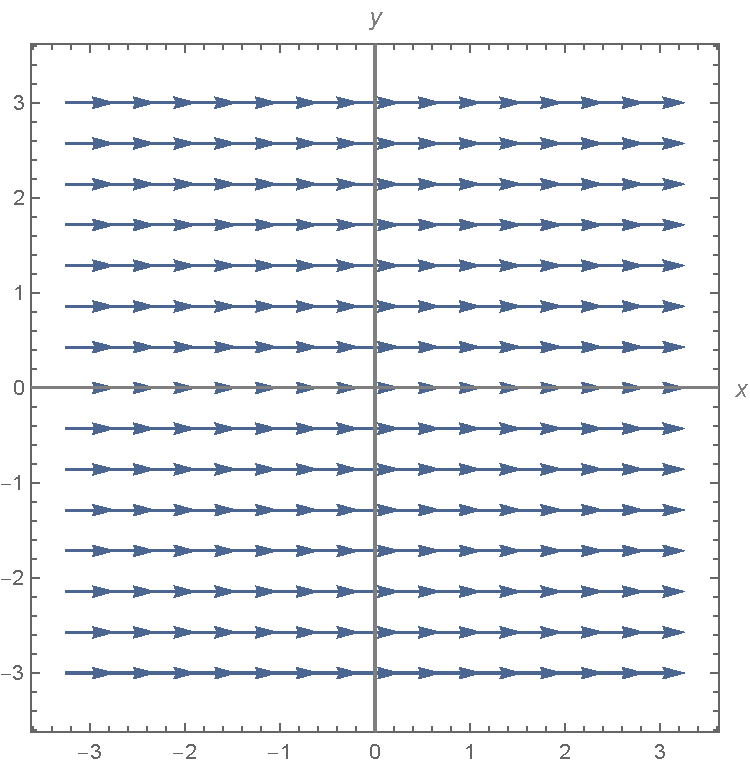
\includegraphics[width=.45\linewidth]{images/vfield_e1.pdf}
     \caption{Vector field v=$e_1=\partial_x$} \label{Fig:vfield_e1}
\end{figure}
\end{definition}



\begin{remarkbox}\begin{remark} [Fields vs. Derivations] \label{fieldsvsder}
  If $v$ is a vector field in $\rfield^n$, then $v$ assigns a vector to another vector of $\rfield^n$. So $v \colon \rfield^n \rightarrow \rfield^n$. So, the set of all vector fields should be (we will use a different symbol to denote it):
  $$X(\rfield^n) = \left \{ v \colon \rfield^n \rightarrow \rfield^n \right \}$$
  However, the definition \ref{setsfields} is a bit different. Why?
  The fact is, we can consider a vector of $\rfield^n$ as a directional derivative, cf. remark \ref{vectorasder} (we are not considering any fixed point here, but the results do not change). Now a derivation, as defined in def. \ref{derivation}, is a map $v \colon C^{\infty}(\rfield^n) \rightarrow \rfield$, i.e. we can say that a derivation is a very smooth element of $\mathbb{F}(\rfield^n) = \{ \text{functions } f \colon \rfield^n \rightarrow \rfield\}$. So, $\mathfrak{X}(\rfield^n) \cong X(\rfield^n)$ because we can associate a derivation of $\mathfrak{X}(\rfield^n)$ to each vector of $X(\rfield^n)$, and vice versa. Then we also explained why in the definition of $\mathfrak{X}( \rfield^n)$ every element must be $\rfield$-linear and satisfy the Leibnitz rule: it follows from the definition of derivations.

  Now, a question arises: given $v$ vector field, should we write $v(p)$ (i.e. it takes vectors as argument) or should we write $v(f)$ (i.e. it takes smooth functions as arguments)? The answer is: it depends on the case, since they are two different "$v$"s. Which is, we will use vectors when we think of $v$ as a function who takes elements of $\rfield^n$, and we will use functions in the other case. And we can choose which case to use, since we can identify every vector field with a derivation, and every derivation with a vector field (for more info, see pag. 181 of \citetalias{Lee}). Now, let us analyze how $v(f)$ is made in the latter case.
  Given $v \in \mathfrak{X}(\rfield^n), f: \rfield^n \rightarrow \rfield$, we define the function $v(f)$ as
  \begin{align} \label{vfpdef}
    v(f) \colon \rfield^n &\rightarrow \rfield \nonumber \\
    p & \mapsto v(f)(p) \equiv v_p f \, .
  \end{align}
  Now, in coordinates:
  \begin{equation} \label{vfieldincoord}
    v(f)(p) = v_p f = v^i(p)(e_i)_p f = v^i(p) \restrict{\frac{\partial}{\partial x^i}}{p} f = v^i(p) \frac{\partial f}{\partial x^i} (p)
  \end{equation}
  where we used summation convention, and the fact that every basis vector $e_i$ can be seen as $\restrict{\partial_{x_i}}{p}$. We defined it in the right way because, as expected, we found that $v_p(f)$ is the directional derivative of $f$ in the direction of $v$, evaluated at $p$. So, in brief:
  \begin{itemize}
    \item $v(f)(p)$ is a number
    \item $v(f)(\cdot)$ is a function from $\rfield^n$ to $\rfield$
    \item $v(\cdot)$ is a function from $\mathbb{F}(\rfield^n)$ to $\mathbb{F}(\rfield^n)$
  \end{itemize}
We also notice that the mathematical object $e_i$ is not much different from $\restrict{(e_i)}{p}$ in this case: there is no difference if we think about them as directions, but it makes a difference if we think about them as directional derivatives, because the latter notation gives info about the point in which the derivative is evaluated. So, we add the pedix "$p$" in order to make the isomorphism between vectors and directional derivatives more explicit. Check also the remark \ref{pointorvec}.
\end{remark}\end{remarkbox}

\begin{figure}[H]
\centering
\begin{subfigure}{.45\textwidth}
     \centering
     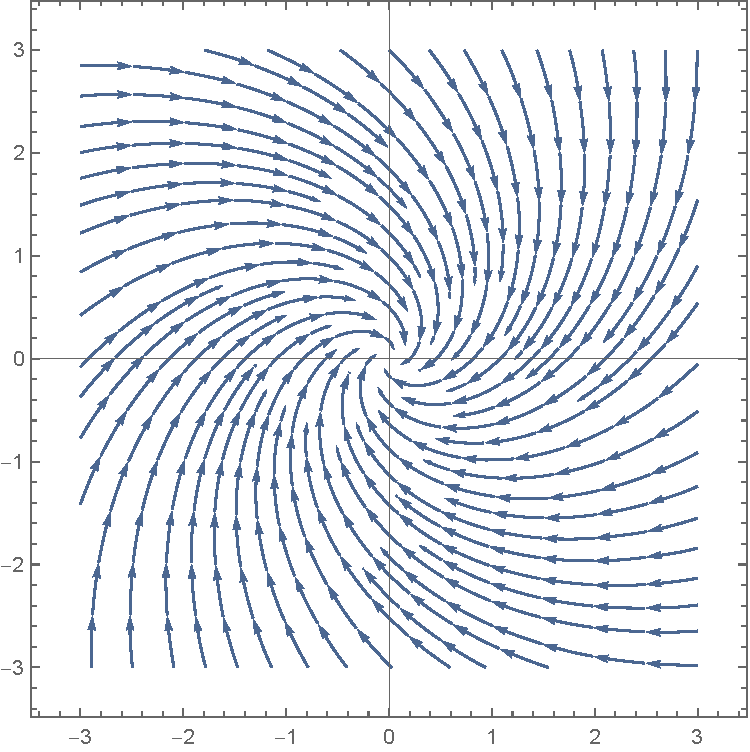
\includegraphics[width=\linewidth]{images/vfield_2.pdf}
     \caption{Vector field v=$(y-x)\partial_x-(y+x)\partial_y$} \label{Fig:vfield_2}
\end{subfigure}
\begin{subfigure}{.45\textwidth}
     \centering
     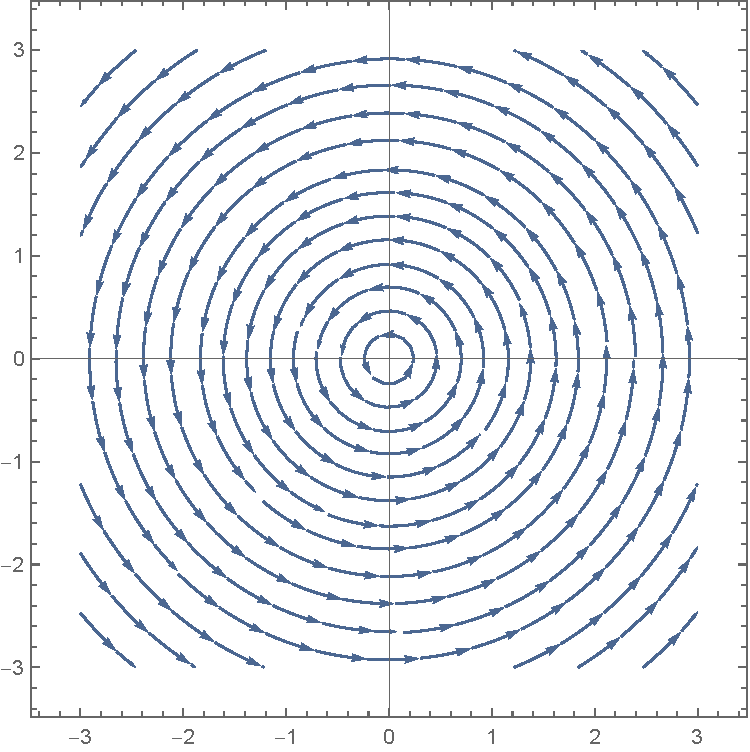
\includegraphics[width=\linewidth]{images/vfield_3.pdf}
     \caption{Vector field v=$-y\partial_x+x\partial_y$} \label{Fig:vfield_3}
\end{subfigure}
\end{figure}

%\begin{remarkbox}\begin{remark}
%So, if $v \in \mathfrak{X}(\rfield^n)$, then $v(f)(p) = \restrict{v(f)}{p} = v^i(p)\restrict{(e_i)}{p} = v^i(p) \restrict{\frac{\partial}{\partial x^i}}{p} f = v^i(p) \frac{\partial}{\partial x^i} f(p)$, where
%\end{remark}\end{remarkbox}
\section[Exterior Product and Generalisation]{\crule[red!50!white]{0.3cm}{0.4cm}  Exterior Product and Generalisation}

\begin{definition} [Exterior form of degree $k$]
Given a vector space $V$ on a field $\mathbb{K}$, with $\dim(V) = n$, and with $k \le n$, an \textit{exterior form of degree $k$} (or $k$-linear form, or $k$-form) is a map $\omega$:
\begin{equation*}
\omega \colon \underbrace{V \times \ldots \times V}_{\text{k times}} \rightarrow \mathbb{K}
\end{equation*}
such that
\begin{equation}
\omega(v_1, \ldots, v_k) = \sgn(\pi)\,\omega(v_{\pi(1)}, \ldots, v_{\pi(k)})
\end{equation}
and such that $\omega$ is multilinear. Where $\pi$ is a permutation of $k$ elements, i.e. $\pi \in S_k$, and $\sgn(\pi)$ is the sign of the permutation.
We will also write $\omega \in \Lambda ^k V^*$.
\end{definition}

\begin{definition}[Exterior product between two 1-forms] \label{extprod}
Given a vector space $V$ on a field $\mathbb{K}, \dim(V) \ge 2$, and given $\varphi^1, \varphi^2 \in \Lambda V^* $, then we define the exterior product (or wedge product) $\wedge$ as:
\begin{align*}
\wedge \colon \Lambda V^* \times \Lambda V^* &\rightarrow \Lambda^2 V^*  \\
(\varphi^1, \varphi^2) &\mapsto \varphi^1 \wedge \varphi^2
\end{align*}
where:
\begin{equation*}
\varphi^1 \wedge \varphi^2 (x_1, x_2) = \varphi^1(x_1) \varphi^2(x_2) - \varphi^2(x_1) \varphi^1(x_2) = \det(\varphi^i (x_j))
\end{equation*}
for $i, j=1,2$.
\end{definition}

\begin{remarkbox}\begin{remark}[Exterior product between $k$ 1-forms]
The exterior product $\wedge$ that we defined for $k=2$ in def. \ref{extprod} gives an exterior form of degree 2. We want to generalize it for $k$ vector spaces. In order to extend the definition, we want it to give an exterior form of degree $k$, so:
\begin{align*}
  \wedge \colon \underbrace{\Lambda V^* \times \ldots \times \Lambda V^*}_{k \text{ times}} &\rightarrow \Lambda^k V^*  \\
  (\varphi^1, \ldots, \varphi^k) &\mapsto \varphi^1 \wedge \ldots \wedge \varphi^k
\end{align*}
where, given $(x_1, \ldots, x_k) \in \underbrace{V \times \ldots \times V}_{k \text{ times}}$:
\begin{equation} \label{detformula}
  \varphi^1 \wedge \ldots \wedge \varphi^k (x_1, \ldots, x_k) =  \det\left (\varphi^i(x_j) \right) \, .
\end{equation}
This is a particular case of an exterior $k$-form (because the sign of determinant changes if we swap two rows or two columns).
Now let's consider an explicit computation using the determinant, in $\rfield^3$, with coordinates $x, y, z$, and with $\varphi^1, \varphi^2, \varphi^3$ corresponding to the three elements of the dual basis $dx \equiv e^{*1} = dx^1, dy \equiv e^{*2} = dx^2$ and $ dz \equiv e^{*3} = dx^3$:
\begin{equation*}
(dx \wedge dy \wedge dz)(x, y, z) = \det\left (dx^i(e_j) \right) = \det \left(
\begin{matrix}
dx(x) & dx(y) & dx(z) \\
dy(x) & dy(y) & dy(z) \\
dz(x) & dz(y) & dz(z)
\end{matrix}
\right )
\end{equation*}
and we can use that $dx^i(e_j) = \delta^i_j$. For instance, we can verify that the 3-form $dx \wedge dy \wedge dz$ gives 0 if two coordinates of the input are repeated:
\begin{equation*}
(dx \wedge dy \wedge dz)(x, x, z) = \det \left(
\begin{matrix}
1 & 1 & 0 \\
0 & 0 & 0 \\
0 & 0 & 1
\end{matrix}
\right ) = 0 \, .
\end{equation*}
\end{remark}\end{remarkbox}



\begin{proposition}\label{basisprop1}
  If $\{e_i\}_{i=1,\ldots,n}$ is a basis in $V$, then $\{e^{*i_1} \wedge \ldots \wedge e^{*i_k}\}_{i_1 < \ldots < i_k, k \le n}$ forms a basis of $\Lambda ^k V^*$.
\end{proposition}
\begin{proof}[Proof]
In the statement we implicitly assumed that the elements of $\{e^{*i_1} \wedge \ldots \wedge e^{*i_k}\}$ are defined as usual, for instance $e^{*i_1}(e_{j_1}) = \delta^{i_1}_{j_1}$. In order to prove that it is a basis, we need to prove that the elements of the basis are linearly independent and that they span the entire space.
\begin{itemize}
\item Linear independence: If
$$0 = \sum\limits_{i_1 < \ldots < i_k} a_{i_1 \cdots i_k} (e^{*i_1} \wedge \ldots \wedge e^{*i_k})(e_{j_1}, \ldots, e_{j_k}), \quad \forall \, (e_{j_1}, \ldots, e_{j_k})$$
then $a_{i_1 \cdots i_k} = 0, \forall\, i_1, \ldots, i_k$. Indeed, if it is true $\forall \, (e_{j_1}, \ldots, e_{j_k})$, then we can choose $e_{j_1}, \ldots, e_{j_k}$ such that $a_{i_1 \cdots i_k} = 0, \forall\, i_1, \ldots, i_k$. e.g.:
\begin{align*}
0 &= a_{i_1 \cdots i_k} \underbrace{(e^{*i_1} \wedge \ldots \wedge e^{*i_k}) (e_{i_1}, \ldots, e_{i_k})}_{= 1} + \\
& + \sum\limits_{\substack{j_1 < \ldots < j_k \\
j_1 \not = i_1, j_2 \not = i_2, \ldots}} a_{j_1 \cdots j_k} \underbrace{(e^{*j_1} \wedge \ldots \wedge e^{*j_k}) (e_{i_1}, \ldots, e_{i_k})}_{= 0} = a_{i_1 \cdots i_k} \, .
\end{align*}
The second term is zero because $(e^{*j_1} \wedge \ldots \wedge e^{*j_k}) (e_{i_1}, \ldots, e_{i_k}) = \det \left (e^{*j_l} (e_{i_m}) \right)$. Indeed, the matrix $e^{*j_l} (e_{i_m})$ has null coefficients on the main diagonal (because $j_1 \not = i_1, j_2 \not = i_2, \ldots$) and one of the rows must be 0 because of  the ordering $j_1 < \ldots < j_k$ and $i_1 < \ldots < i_k$ (e.g. consider the case $j_2 = i_1, \ldots$). Thus, the determinant is 0.
Therefore, $a_{i_1 \cdots i_k} = 0$.
So, we proved the linear independence in case we consider the basis vectors $e_{j_1}, \ldots, e_{j_k}$. Because of multilinearity, the result holds for all vectors
 $(x_1, \ldots, x_k)$ as well.
\item Completeness: given $\psi \in \Lambda^k V^*$, we want to prove that there exists a coefficient $a_{i_1 \cdots i_k}$ such that $\psi = \sum\limits_{i_1 < \ldots < i_k} a_{i_1 \cdots i_k} (e^{*i_1} \wedge \ldots \wedge e^{*i_k})$, i.e. we want to prove that we can write any element of $\Lambda^k V^*$ as a linear combination of elements of $\{e^{*i_1} \wedge \ldots \wedge e^{*i_k}\}$. Let's consider $(v_1, \ldots v_k) \in V \times \ldots \times V$. Then:
\begin{align*}
\psi(v_1, \ldots, v_k) &\overset{(1)}{=} \sum\limits_{i_1 = 1}^k \sum\limits_{i_2 = 1}^k \ldots \sum\limits_{i_k = 1}^k x_{i_1} \cdot \ldots \cdot x_{i_k} \psi(e_{i_1}, \ldots, e_{i_k}) \overset{(2)}{=} \\
&= \sum\limits_{i_1 < \ldots < i_k} x_{i_1} \cdot \ldots \cdot x_{i_k} \psi(e_{i_1}, \ldots, e_{i_k}) \overset{(3)}{=} \\
&= \sum\limits_{i_1 < \ldots < i_k} x_{i_1} \cdot \ldots \cdot x_{i_k} \psi(e_{i_1}, \ldots, e_{i_k}) (e^{*i_1} \wedge \ldots \wedge e^{*i_k}) (e_{i_1}, \ldots, e_{i_k}) \overset{(4)}{=} \\
&= \sum\limits_{i_1 < \ldots < i_k} \psi(e_{i_1}, \ldots, e_{i_k}) (e^{*i_1} \wedge \ldots \wedge e^{*i_k}) (x_{i_1}e_{i_1}, \ldots, x_{i_k}e_{i_k}) \overset{(5)}{=} \\
&= \sum\limits_{i_1 < \ldots < i_k} a_{i_1 \cdots i_k}(e^{*i_1} \wedge \ldots \wedge e^{*i_k}) (v_1, \ldots, v_k) \, .
\end{align*}
Where we used: (1) $v_1 = \sum\limits_{i_1 = 1}^k x_{i_1}e_{i_1}$ in the $\{e_i\}_{i=1}^n$ basis, (2) we can simplify the sum since $\psi=0$ if two entries are repeated (and any sign is absorbed in the coefficients $x_i$), (3) $1 = (e^{*i_1} \wedge \ldots \wedge e^{*i_k}) (e_{i_1}, \ldots, e_{i_k})$, (4) multilinearity, (5) $0 = e^{*i}(e_j)$ if $i \not = j$ and $a_{i_1 \cdots i_k} \equiv \psi(e_{i_1}, \ldots e_{i_k})$. \qedhere
\end{itemize}
\end{proof}

\begin{remarkbox}\begin{remark}
  The above proposition proves that $\dim(\Lambda^k V^*)=\binom{n}{k}$, because through the expression "$i_1 < \ldots < i_k, \, k \le n$" we are selecting subsets of $k$ elements (subsets, not $k$-tuples, because the order of the elements is externally fixed) from a bigger set of $n$ elements. This is exactly the definition of the binomial coefficient $\binom{n}{k}$. Moreover, it means that any $\alpha \in \Lambda^k V^*$ can be written as:
  \begin{equation*}
    \alpha = \sum\limits_{i_1 < \ldots < i_k} a_{i_1 \cdots i_k} e^{*i_1} \wedge \cdots \wedge e^{*i_k}
  \end{equation*}
  where $a_{i_1 \cdots i_k} \in \mathbb{K}$, $\mathbb{K}$ field of the vector space.
\end{remark}\end{remarkbox}

Now, we want to define the exterior product between a $k$-form and a $p$-form (and it will return a ($p+k$)-form).

\begin{definition}[Exterior product between a $k$-form and a $p$-form]
  Given $\alpha \in \Lambda ^k V^*, \beta \in \Lambda^p V^*$, the exterior product between them is defined as:
  \begin{align}
    \wedge \colon \Lambda ^k V^* \times \Lambda ^p V^* &\rightarrow \Lambda^{k+p} V^* \nonumber \\
    (\alpha, \beta) &\mapsto \alpha \wedge \beta \nonumber
  \end{align}
  with:
  $$\alpha \wedge \beta = \sum\limits_{\substack{i_1 < \ldots < i_k \\ j_1 < \ldots < j_p}} \alpha_{i_1 \cdots i_k}\beta_{j_1 \cdots j_p} e^{*i_1} \wedge \cdots \wedge e^{*i_k} \wedge e^{*j_1} \wedge \cdots \wedge e^{*j_p} $$
  where $\alpha_{i_1 \cdots i_k},\beta_{j_1 \cdots j_p} \in \mathbb{K}$.
\end{definition}


\begin{tcolorbox}\begin{example}[Oriented area] \label{orarea}
  Let's consider the following examples:
  \begin{enumerate}
    \item Let's suppose our space is $V = \rfield^3 \times \rfield^3$ with cartesian coordinates.
    $$\varphi \equiv dx^1 \wedge dx^2 + dx^2 \wedge dx^4$$
    where $\varphi$ is a sum of two 2-forms. They are 2-forms (and not 1-forms, nor 3-forms, nor 4-forms, ...) because they are written as wedge product ("$\wedge$") of \textbf{two} elements of the dual basis. Remember that we denote the elements of the dual basis either by $e^{*i}$ or $dx^i$ for some $i$.
    Let's compute $\varphi(e_i, e_j)$. We can use the determinant formula \eqref{detformula}:
\begin{align*}
    \varphi(e_i, e_j) = &dx^1(e_i) dx^2(e_j) + dx^2(e_i)dx^4(e_j) - dx^2(e_i)dx^1(e_j) + \\ - &dx^4(e_i)dx^2(e_j)\, .
    \end{align*}
    \item Let's consider $V = \rfield^2$ with cartesian coordinates $x^1, x^2$. Let:
    $$\varphi \equiv dx^1 \wedge dx^2\, .$$
    Let's compute $\varphi(ae_1, be_2)$, where $ a,b \in \rfield$:
    \begin{align*}
    \varphi(ae_1, be_2) &= dx^1 \wedge dx^2(ae_1, be_2) = ab\,  dx^1 \wedge dx^2(e_1, e_2) = \\
    &= ab \, (dx^1(e_1)dx^2(e_2) - \cancel{dx^2(e_1)} \cancel{dx^1(e^2)}) = ab = \\
    &= \text{oriented area of the rectangle of sides } a \text{ and } b\, .
  \end{align*}
  \end{enumerate}

\end{example}\end{tcolorbox}

There are some interesting properties about $k$-forms:
\begin{proposition}
  $\alpha \in \Lambda^k V^*, \beta \in \Lambda^p V^*, \gamma \in \Lambda ^q V^*$, then:
  \begin{enumerate}
    \item $(\alpha \wedge \beta) \wedge \gamma = \alpha \wedge (\beta \wedge \gamma)$,
    \item $\alpha \wedge (\beta + \gamma) = \alpha \wedge \beta + \alpha \wedge \gamma$,
    \item $\alpha \wedge \beta = (-1)^{kp} \beta \wedge \alpha$.
  \end{enumerate}
\end{proposition}
\begin{proof}[Sketch of the proof]
$ $
	\begin{enumerate}
	\item Writing the forms in terms of the basis, we only need to prove that the property (1) holds for the elements of the dual basis. Moreover, by multilinearity, we just need to prove it for the elements of the dual basis applied to a basis $\{e_i\}$ of $V$. Thus, the proof for (1) is over because this property is true for the determinant: when we compute it, we can start from any row or column.
	\item By writing the forms in terms of the basis as before.
	\item  Again, by writing the forms in terms of the basis we have a sequence of wedge products like
	$$e^{*i_1} \wedge \ldots \wedge e^{*i_k} \wedge e^{*j_1} \wedge \ldots \wedge e^{*j_p}\, .$$
	If we swap two elements of the product we get a factor "$-1$". In order to have the right hand side we need to "move $e^{*j_1}$ on the left $k$ times", so we get a factor $(-1)^k$. Same for $e^{*j_2}$: we need to move it on the left $k$ times and so we get an extra factor $(-1)^k$. Again, we repeat the procedure for all the elements up to $e^{*j_p}$. At the end, we get a factor $(-1)^{kp}$. \qedhere
	\end{enumerate}
\end{proof}

\section[Differential Forms]{\crule[purple!50!white]{0.3cm}{0.4cm}  Differential Forms}
\begin{definition} [Field of exterior forms, geometric definition] \label{geomkforms}
  (A field of) exterior forms of degree $k$, $k \le n$ is a map $\omega$ that associates to each point $p \in V$ an element $\omega(p) \in \Lambda^{k}V_p^*$.
  Choosing a basis, we have:
  \begin{equation} \label{kformdef}
    \omega(p) = \sum\limits_{i_1 < \ldots < i_k} \underbrace{a_{i_1 \cdots i_k}(p)}_{\text{now it is a function!}} e^{*i_1} \wedge \cdots \wedge e^{*i_k} \, .
    \end{equation}
    The form $\omega$ is a differential form if $a_{i_1 \cdots i_k}$ are differentiable functions. The set of differential $k$-forms with coefficients in $\rfield^n$ is denoted by $\Omega^k(\rfield^n)$.
\end{definition}

Another (equivalent) definition:

\begin{definition} [Algebraic definition of differential $k$-form] \label{algkforms}
  A differential $k$-form is a map:
  \begin{align}
    \omega \colon \underbrace{\mathfrak{X}(\rfield^n) \times \ldots \times \mathfrak{X}(\rfield^n)}_{k \text{ times}} \rightarrow \mathbb{F}(\rfield^n)
  \end{align}
  $C^\infty(\rfield^n)$-linear and alternating.
\end{definition}

\begin{remarkbox}\begin{remark}
  To show the equivalence of the two definition of differential $k$-forms we just need to show that:
  \begin{equation}
    \omega(p)(v_1, \ldots, v_k) = \omega(v_1, \ldots, v_k)(p) \, .
  \end{equation}
  See also the exercise 1, problem sheet 3.
\end{remark}\end{remarkbox}

We want to generalize the concept of differential of a function.
\begin{definition}[Differential] \label{differential}
  Let $f$ be a function $f \colon U \subseteq \rfield^n \rightarrow \rfield$, $f$ differentiable. Let $v \in \mathfrak{X}(\rfield^n) = \Der \mathbb{F}(\rfield^n)$. The exterior derivative of $f$ is its differential $d$, defined as a 1-form such that:
  \begin{equation}
    df(v) = v(f) \, .
  \end{equation}
\end{definition}

\begin{remarkbox}\begin{remark}[Differential expression in coordinates] \label{diffcoordremark}
  We want to verify that the above definition of differential is equivalent to our usual definition for $C^1(\rfield^n)$ function, which is:
  \begin{equation}
    df = \sum\limits_{i=1}^n \frac{\partial f}{\partial x_i} dx^i = \frac{\partial f}{\partial x_i} dx^i \, .
  \end{equation}
  In order to prove that, we first consider a pointwise definition. Given $p \in \rfield^n$:
  \begin{equation} \label{diffdefp}
    df_p(v) = v(f), \forall\,\, v \in T_p \rfield^n \cong \rfield^n \, .
  \end{equation}
  ($T_p \rfield^n$ is the tangent space to $\rfield^n$ at $p$). Now, we can write $v(f)$ in coordinates (the gray part is the one we don't care about):
  \begin{equation} \label{diffcoordinates}
    df_p = \textcolor{lightgray}{v(f) = \text{ }} v_i(p) (\lambda^i)_p
  \end{equation}
  where $(\lambda^i)_p$ is a dual basis at $p$ (later, we will prove that $(\lambda^i)_p = (dx^i)_p$). Now, applying $df$ to a particular vector (i.e. directional derivative) at $p$:
  \begin{equation} \label{diffpart1}
    df_p \left (\restrict{\frac{\partial}{\partial x^i}} {p} \right) = v_i(p)
  \end{equation}
  where we used the property of the dual basis
  \begin{equation}
    (\lambda^i)_p \restrict{\frac{\partial}{\partial x^j}} {p} = \delta^i_j
  \end{equation}
   and then:
   \begin{equation}
   \textcolor{lightgray}{df_p \left (\restrict{\frac{\partial}{\partial x^i}} {p} \right) = \text{ }} v_i(p) (\lambda^i)_p \restrict{\frac{\partial}{\partial x^i}} {p} = v_i(p) \, .
 \end{equation}
   On the other hand, by definition \eqref{diffdefp} we know that:
   \begin{equation} \label{diffpart2}
     df_p \left (\restrict{\frac{\partial}{\partial x^i}} {p} \right)  = \restrict{\frac{\partial}{\partial x^i}} {p} f = \frac{\partial f}{\partial x^i} (p) \, .
   \end{equation}
   Hence, using \eqref{diffpart1} and \eqref{diffpart2} we get:
   \begin{equation}
     v_i (p) = \frac{\partial f}{\partial x^i} (p) \, .
   \end{equation}
   Then, by the expression of differential in coordinates \eqref{diffcoordinates}:
   \begin{equation}
     df_p = \frac{\partial f}{\partial x^i} (p) (\lambda^i)_p\, .
   \end{equation}
   Applying the definition to $f = x^j$ (coordinate function, as defined in \eqref{coofunc}), we get:
   \begin{equation}
     df_p = \frac{\partial f}{\partial x^i} (p) (\lambda^i)_p = \frac{\partial f}{\partial x^i} (p) (dx^i)_p \, .
   \end{equation}
   And then:
   \begin{equation}
     df = \frac{\partial f}{\partial x^i} dx^i\, .
   \end{equation}
   Indeed, if $f = x^j$ then, as before:
   \begin{equation}
     (dx^j)_p = \frac{\partial x^j}{\partial x^i} (p) \restrict{(\lambda^i)}{p} = \delta^i_j \restrict{(\lambda^i)}{p} = \restrict{(\lambda^j)}{p} \, .
   \end{equation}
Pay attention: what we did here is a bit different from what we did for the definition $\ref{vfpdef}$ of a vector field applied to a function. In this case, $p$ is the point where we fixed our vector, whereas in the other case $p$ was the point where we wanted to evaluate the directional derivative of $f$.
\end{remark}\end{remarkbox}

In the above definition, $f$ was a 0-form (i.e. a function). What is the generalization of the differential to $k$-forms?

\begin{definition}[Exterior derivative] \label{extder}
  If $k > 0$, then the exterior derivative (acting on $k$-forms) is a map
  \begin{align*}
    d \colon \Omega^k(\rfield^n) & \rightarrow \Omega^{k+1}(\rfield^n) \\
    \omega &\mapsto d (\omega) \equiv d \omega
  \end{align*}
  where
  \begin{equation*}
    d \omega = \sum\limits_{j_1 < \ldots < j_k} \left (d a_{j_1, \ldots, j_k} \right) \wedge dx^{j_1} \wedge \ldots \wedge dx^{j_k}
  \end{equation*}
with $d a_{j_1, \ldots, j_k}$ differential of the function $a_{j_1, \ldots, j_k}$.
\end{definition}

\begin{tcolorbox}\begin{example}[Computation of $d\omega$]
  Let's consider the following examples:
  \begin{enumerate}
    \item Let $\omega$ be a 2-form on $\rfield^3$ (coordinates $x^1, x^2, x^3$):
    $$\omega = dx^1 \wedge dx^2 + x^2 dx^1 \wedge dx^3\, .$$
    Then:
    $$d \omega = dx^2 \wedge dx^1 \wedge dx^3$$
    where we used that "$d (dx^1 \wedge dx^2) = 0$" because there is no 3-form on a 2-dimensional space. (otherwise, we can use that $d^2=0$, but we still have to prove it!)
    \item In $\rfield^n$, let's consider:
    $$\omega = x^2 dx^1 \, .$$
    We have:
    $$ d \omega = dx^2 \wedge dx^1$$
    where we used the definition \ref{extder}. Moreover, if $u,v \in \mathfrak{\rfield^n}$, then by definition of exterior product we have:
    $$d \omega (u, v) = dx^2(u)dx^1(v) - dx^2(v)dx^1(u)\, .$$
    On the other hand, using that $d g(v) = v(g)$ for a function $g$ and a vector field $v$, we have:
    \begin{align*}
    dx^2(u)&=u(x^2)\, , \\
    v(x^2) &= dx^2(v)
    \end{align*}
where $x^2$ is a function, the coordinate function defined in \eqref{coofunc}. We also have:
    $$d \omega (u, v) = u(x^2)dx^1(v) - v(x^2)dx^1(u) \, .$$
  \end{enumerate}
\end{example}\end{tcolorbox}

Now, some properties:
\begin{proposition}[Properties of exterior derivatives]
  $\omega_1 \in \Omega^k(\rfield^n), \omega_2 \in \Omega^p(\rfield^n)$. Then:
  \begin{itemize}
    \item $d(\omega_1 +\omega_2) = d\omega_1 + d\omega_2$,
    \item $d(\omega_1 \wedge \omega_2) = d\omega_1 \wedge \omega_2 + (-1)^k \omega_1 \wedge d\omega_2$,
    \item $d(d\omega_1)  = 0 = d(d\omega_2)$.
  \end{itemize}
\end{proposition}
\begin{proof}[Sketch of the proof]
$ $
	\begin{itemize}
	\item We have
	$$d \omega_1 = \sum\limits_{j_1 < \ldots < j_k} \left (d a^{(1)}_{j_1 \cdots j_k} \right) \wedge dx^{j_1} \wedge \ldots \wedge dx^{j_k}$$
	and similarly for $\omega_2$. Then we use the linearity of the differential: $d(a^{(1)} + a^{(2)}) = da^{(1)} + da^{(2)}$.
	\item We have
	$$d(\omega_1 \wedge \omega_2) = \sum\limits_{\substack{j_1 < \ldots < j_k \\ i_1 < \ldots < i_p}} d \left (a^{(1)}_{j_1 \cdots j_k} a^{(2)}_{i_1 \cdots i_p} \right) \wedge dx^{j_1} \wedge \ldots \wedge dx^{j_k} \wedge dx^{i_1} \wedge \ldots \wedge dx^{i_p} \, .$$
	Using the product rule we have a term $\left ( da^{(1)} \right ) a^{(2)} + a^{(1)} \left(da^{(2)}\right)$ inside the sum. Now, $\left( da^{(1)} \right) a^{(2)}$ gives the term $d \omega_1 \wedge \omega_2$. In order to get the term $(-1)^k \omega_1 \wedge d \omega_2$ we consider $a^{(1)}\left(da^{(2)} \right) \wedge dx^{j_1} \wedge \ldots \wedge dx^{j_k} \wedge dx^{i_1} \wedge \ldots \wedge dx^{i_p}$ inside the sum and we move the factor $da^{(2)}$ to the right for $k$ times. So we get the factor $(-1)^k$) and the wedge product $\omega_1 \wedge d \omega_2$.
	\item Let's consider
	$$d(d \omega) = \sum\limits_{j_1 < \ldots < j_k} d \left (da_{j_1 \cdots j_k} \right) \wedge dx^{j_1} \wedge \ldots \wedge dx^{j_k} \, .$$
	Now,
	$$da_{j_1 \cdots j_k} = \left(\frac{\partial}{\partial x^l} a_{j_1 \cdots j_k} \right)dx^l$$
	and:
	$$\left[d \left( \frac{\partial}{\partial x^l} a_{j_1 \cdots j_k}\right) \right] dx^l = \underbrace{\frac{\partial^2}{\partial x^m \partial x^l} a_{j_1 \cdots j_k}}_{\text{symmetric in } l \leftrightarrow m} \, \underbrace{dx^m \wedge dx^l}_{\text{antisymmetric in } l \leftrightarrow m} \, .$$
	Then we get a minus sign if we exchange $l$ and $m$. Moreover we can compute  $\left[d \left( \frac{\partial}{\partial x^m} a_{j_1 \cdots j_k}\right) \right] dx^m$ in the same way exchanging the roles of $l$ and $m$, and we wouldn't get any minus sign. Then we have that $d(d \omega) = -d (d \omega) \Rightarrow d(d \omega) = 0$. \qedhere
	\end{itemize}
\end{proof}

\begin{remarkbox}\begin{remark} \label{abusenot1}
  In the above proposition, we claimed that $d(d\omega)  = 0$ if $\omega \in \Omega^k(\rfield^n)$. The notation here is not the most precise, since the inner "d" is acting on a $k$-form, whereas the outer "d" is acting on a ($k+1$)-form (so, even if they share the same name, they are different maps). However the behaviour of both "d"s is clear, so we will continue with this abuse of notation.
\end{remark}\end{remarkbox}

\begin{remarkbox}\begin{remark}
  The exterior derivative increases the degree of a $k$-form by 1 (the $k$-form becomes a ($k+1$)-form). Can we get backwards, which is, can we decrease the degree of a $k$-form? Yes, using the interior derivative.
\end{remark}\end{remarkbox}

\begin{definition}[Interior derivative] \label{intder}
  Let $z$ be a vector field on $\rfield^n$, i.e. $z \in \mathfrak{X}(\rfield^n)$, then we define the \textit{interior derivative} $i_z$ (acting on differential $k$-forms) as the map:
  \begin{align}
    i_z \colon \Omega^k(\rfield^n) &\rightarrow \Omega^{k-1}(\rfield^n) \\
    \omega &\mapsto i_z(\omega) \equiv i_z \omega \nonumber
  \end{align}
  such that
  $$(i_z \omega) (v_1, \ldots, v_{k-1}) = \omega(z, v_1, \ldots, v_{k-1}), \forall \, v_i \in \mathfrak{X}(\rfield^n) \, .$$
  $i_z \omega$ is also called  \textit{contraction} or \textit{interior multiplication}. Another notation for $i_z \omega$ is $z \, \lrcorner \, \omega$.
\end{definition}

\begin{tcolorbox}\begin{example}[Some computations]
  In $\rfield^2$, Let $e_x, e_y$ be the basis vectors (that can be seen as vector fields). Then we have:
  $$i_{e_x}(dx \wedge dy) = dy,$$
  $$i_{e_y}(dx \wedge dy) = - dx \, .$$
\end{example}\end{tcolorbox}

\begin{remarkbox}\begin{remark}
  In the definition \ref{intder} above, we used the algebraic definition of differential $k$-forms, i.e. definition \ref{algkforms}.
\end{remark}\end{remarkbox}

Now some properties for interior derivatives.

\begin{proposition}
 Let $\omega \in \Omega^k(\rfield^n), \eta \in \Omega^p(\rfield^n), z \in \mathfrak{X}(\rfield^n)$, then:
  \begin{itemize}
    \item $i_z (\omega \wedge \eta) = (i_z \omega) \wedge \eta + (-1)^k \omega \wedge (i_z \eta)$,
    \item $i_z^2 w = i_z(i_z \omega) = 0$.
  \end{itemize}
\end{proposition}
\begin{proof}[Sketch of the proof]
$ $
\begin{itemize}
\item First, we assume $k+p \le n$, otherwise $\omega \wedge \eta$ would be 0. Then, let's consider a basis $\mathcal{B} = \{e_1, \ldots, e_n\}$ in $\rfield^n$ which is positively oriented (i.e. if $A$ is the matrix that we use to change coordinates from the canonical basis to $\mathcal{B}$, we have $\det A > 0$). Let's choose $\mathcal{B}$ such that the vector field $e_1$ is the tangent vector to the vector field $z$ in one point (we will make a pointwise reasoning). Moreover, $\{dx^l\}_{l=1}^n$ is the dual basis with respect to the canonical basis, and $\{e^{*l}\}_{l=1}^n$ is the dual basis with respect to $\mathcal{B}$. We have
$$\omega = \sum\limits_{i_1 < \ldots < i_k} a_{i_1 \cdots i_k} dx^{i_1} \wedge \ldots \wedge dx^{i_k}$$
and
$$\omega \wedge \eta = \sum\limits_{\substack{i_1 < \ldots < i_k \\ j_1 < \ldots < j_p }} a_{i_1 \cdots i_k} b_{j_1 \cdots j_p} dx^{i_1} \wedge \ldots \wedge dx^{i_k} \wedge dx^{j_1} \wedge \ldots \wedge dx^{j_p} \, .$$
Then either:
\begin{enumerate}
\item $dx^{i_r} = e^{*1}$ for some $i_r, r= 1, \ldots, k$, or
\item $dx^{j_r} = e^{*1}$ for some $j_r, r= 1, \ldots, p$, or
\item there are no $i_r, j_r$ such that "$dx^{i_r} = e^{*1}$ or $dx^{j_r} = e^{*1}$".
\end{enumerate}
So, $i_z (\omega \wedge \eta) = (\omega \wedge \eta)(z, \ldots)$ is either equal to:
\begin{enumerate}
\item $\sum\limits_{\substack{i_1 < \ldots < i_k \\ j_1 < \ldots < j_p }} a_{i_1 \cdots i_k} b_{j_1 \cdots j_p} i_z \left( dx^{i_1} \wedge \ldots \wedge dx^{i_k} \right ) \wedge dx^{j_1} \wedge \ldots \wedge dx^{j_p}$, because the only non-zero term comes from $i_z(e^{*1}) = e^{*1}(z) = e^{*1}(e_1) = 1$ (locally), and we know that the non-zero term must be hidden in the first $k$ wedge products, or
\item $\sum\limits_{\substack{i_1 < \ldots < i_k \\ j_1 < \ldots < j_p }} (-1)^k a_{i_1 \cdots i_k} b_{j_1 \cdots j_p}  dx^{i_1} \wedge \ldots \wedge dx^{i_k}  \wedge i_z \left( dx^{j_1} \wedge \ldots \wedge dx^{j_p} \right)$ , for the same reason above, and we have the factor $(-1)^k$ because we moved the interior derivative $k$ times (it is like moving an entry of a $(k+p)$-form $k$ times), or
\item 0.
\end{enumerate}
Then, $i_z(\omega \wedge \eta)$ is the sum of these possible terms.
\item Using the fact that a differential form gives 0 if two or more entries are repeated:
$$i_z \left( i_z(\omega) \right) (v_1, \ldots, v_{k-2}) = i_z \omega (z, v_1, \ldots, v_{k-2}) = \omega (z, z, v_1, \ldots, v_{k-2}) = 0 \, .$$ \qedhere
\end{itemize}
\end{proof}

\begin{remarkbox}\begin{remark}
  In the above proposition there is a little abuse of notation when we claimed $i_z(i_z \omega) = 0$, see also the remark \ref{abusenot1}.
\end{remark}\end{remarkbox}

\begin{definition}[Nondegenerate 2-form]
An exterior form $\omega$ of degree 2 on a vector space $V$, $\omega \in \Lambda^2V^*$, is said to be nondegenerate if the map from $V$ to $V^*$ defined as $z \mapsto i_z \omega$ is invertible.
\end{definition}

\begin{remarkbox}\begin{remark}[Alternative definitions of nondegenerate form]
The following ones are equivalent:
\begin{enumerate}
\item $\omega$ is non degenerate,
\item for each nonzero $v \in V$, there exists $w \in V$ such that $\omega(v, w) \ne 0$,
\item in terms of some basis, the matrix $(\omega_{ij})$ representing $\omega$ is nonsingular.
\end{enumerate}

\end{remark}\end{remarkbox}

Now, let's talk about \textit{pullbacks} and \textit{pushforwards} for functions and $k$-forms.

\begin{definition}[Pullback]
  Let $f \colon U \rightarrow V$ (with $U, V \subseteq \rfield^n$) be a differentiable map. Let's suppose that $\dim(U) = \dim(V) = n$ (just for the sake of simplicity, since it is not necessary). Then the \textit{pullback} of a $k$-form (from $V$) to $U$ is the map:
  \begin{align*} \label{pullbackdef}
    f^* \colon \Omega^k(V) & \rightarrow \Omega^k(U) \\
    \omega & \mapsto f^*w
  \end{align*}
  such that
  \begin{equation*}
    (f^* \omega)(p) (u_1, \ldots, u_k) = \omega (f(p)) (df(u_1), \ldots, df(u_k)), \quad \forall\, \, p \in \rfield^n, \forall \,\, u_i \in \mathfrak{X}(U) \, .
  \end{equation*}
\end{definition}

Now, we want to give another name to the differential of a function.
\begin{definition}[Pushforward]
  Given $f \colon U \rightarrow V$ as before, we will also call the differential of $f$ at $p \in \rfield^n$, i.e. $df_p = df(p)$, as the \textit{pushforward} of $f$ at $p$, and it will be denoted by the symbol $(f_*)_p$.
  So, the pushforward map is:
\begin{align*}
  df_p \equiv (f_*)_p \colon U \subset \rfield^n &\rightarrow V \subset \rfield^m \\
    v & \mapsto (f_*)_p (v) \, .
\end{align*}
\end{definition}

\begin{remarkbox}\begin{remark}[Pushforward of composition of functions] \label{pushfcomposition}
In our mind, we'll think of the pushforward as the differential of a map: $df_p = (f_*)_p$, at least until this concept is generalized.
By definition of differential: $df_p(v) = v(f)$, where $v$ is a vector tangent to $\rfield^n$ at $p$. Since vectors are like directional derivatives, $v(f)$ is the directional derivative of $f$ with respect to $v$ (not evaluated at any point, for now!). In particular, if we apply the definition to a point $h(q)$, where $h \in C^{\infty}(\rfield^n, \rfield^m)$ and $q \in \rfield^n$, we have (cf. also pag. 55 Lee \citetalias{Lee}):
$$\restrict{(f_*)_p (v)(h)}{q} \overset{(1)}{=} \restrict{v(h \circ f)}{q}  = \restrict{v(h(f))}{q} \overset{(2)}{=} \restrict{v (f^* h) }{q}$$
where we used: (1) $(f_*)_p (v)(h)  = v(h \circ f)$, it can be proved that it is the right expression in a similar way to what we did to prove that $(f_*)_p (v)= v(f)$ is the right expression (cf. remark \ref{diffcoordremark}), (2) the expression of the pullback for a differentiable function, which is completely legal since we defined it for differentiable $k$-forms, and a differentiable function is just a 0-form.
\end{remark}\end{remarkbox}

\begin{remarkbox}\begin{remark}
Using the pushforward, we can define the pullback of a differential form using a different notation (i.e. using $f_*$ instead of $df$):
  \begin{equation}
    (f^* \omega)(p) (u_1, \ldots, u_k) = \omega (f(p)) (f_*(u_1), \ldots, f_*(u_k)), \forall\, \, p \in \rfield^n, \forall \,\, u_i \in \mathfrak{X}(U)
  \end{equation}
\end{remark}\end{remarkbox}

Now, some properties of the pullback.

\begin{proposition} \label{pullbackprop}
  Let $g, f \in C^1(\rfield^n, \rfield)$, $\omega, \varphi \in \Omega^k(\rfield^n)$, $h\colon \rfield^n \rightarrow \rfield$. Then:
  \begin{enumerate}
    \item $f^*(\omega + \varphi) = f^*(\omega) + f^*(\varphi)$,
    \item $f^*(h \omega) = f^*(h)f^*(\omega)$,
    \item $(f \circ g)^* = g^*(f^*(\omega))$,
    \item If $\varphi^1, \ldots, \varphi^k \in \Omega^1(\rfield^n)$, then $f^*(\varphi^1 \wedge \ldots \wedge \varphi^k) = f^*(\varphi^1) \wedge \ldots \wedge f^*(\varphi^k)$,
    \item $df^*(\omega) = f^*(d\omega)$.
  \end{enumerate}
  From property (4) also follows that $f^*(\omega \wedge \phi) = (f^*\omega) \wedge (f^* \phi)$
\end{proposition}
\begin{proof}[Sketch of the proof]
$ $
\begin{enumerate}
\item \begin{align*}
f^*(\omega + \varphi) &= (\omega + \varphi)(f(p)) (f_*(u_1), \ldots, f_*(u_k)) =\\
& = \omega(f(p)) (f_*(u_1), \ldots, f_*(u_k)) + \varphi(f(p)) (f_*(u_1), \ldots, f_*(u_k)) = \\
&=  f^*(\omega) + f^*(\varphi) \, .
\end{align*}
\item $f^*(h \omega) (z_1, \ldots, z_k)(p) = h(f(p))\, \omega (f_* z_1, \ldots, f_* z_k) (f(p)) = f^*(h)f^*(\omega)$.
\item We will use: $(f \circ g)_* v(h) = v \left ( (f \circ g)^* h \right) = v(g^* \circ f^*(h)) \overset{(1)}{=} g_*v(f^*h) = f_* \tilde v (h) = f_* \circ g_* v$, where $\tilde v \equiv g_* v$.  In (1) we used $v(h \circ f) = f_* (v \circ h)$ with $f, h$ differentiable functions, $v$ smooth vector field (see remark \ref{pushfcomposition}). Then:
\begin{align*}
(f \circ g)^* \omega(z_1, \ldots, z_k) &= \omega ((f \circ g)_* z_1, \ldots, (f \circ g)_* z_k)) = \omega(f_* \circ g_* z_1, \ldots, f_* \circ g_* z_k) = \\ &= g^*(f^* \omega)(z_1, \ldots, z_k) \, .
\end{align*}
\item We have: \begin{align*}
f^*(\varphi^1 \wedge \ldots \wedge\varphi^k)(z_1, \ldots, z_k) &= (\varphi^1 \wedge \ldots \wedge \varphi^k)(f_* z_1, \ldots, f_*z_k) = \det\left( \varphi^i (f_* z_j)\right) = \\
&= \det \left( f^* \varphi^i(z_j) \right) = (f^* \varphi^1)\wedge \ldots \wedge (f^* \varphi^k) \, (z_1, \ldots, z_k) \, .
\end{align*}
\item If $z$ is a vector field and $dx^i$ is an element of the dual basis (in particular, $dx^i(e_j) = \frac{\partial}{\partial x^j} x^i$), we have
$$f^*dx^i(z) = dx^i(f_* z) \overset{(A)}{=} z(f^i) = df^i(z)$$
where in (A) we used: 
\[ dx^i(f_* z) = f_* z(x^i) \text{ because of the definition } df(v) = v(f)\, . \]
Moreover,
\[ f_* z(x^i) = f_*(z \circ x^i) = z(x^i \circ f) \text{ by the property } f_*(v \circ h) = v(h \circ f) \, .\]
Finally,
\[ z(x^i \circ f) = z(f^i) \, . \]
In the last equality we used the def. \ref{differential} of differential. 
Now,
\begin{align*}
df^*(\omega) &= df^* \left(\sum\limits_{i_1 < \ldots < i_k} a_{i_1 \cdots i_k} dx^{i_1} \wedge \ldots \wedge dx^{i_k} \right) = \\
&= d \, \sum\limits_{i_1 < \ldots < i_k} f^* (a_{i_1 \cdots i_k}) f^*(dx^{i_1}) \wedge \ldots \wedge f^*(dx^{i_k}) \overset{(1)}{=} \\
&=\sum\limits_{i_1 < \ldots < i_k} df^*(a_{i_1 \cdots i_k}) \wedge df^{i_1} \wedge \ldots \wedge df^{i_k} \overset{(2)}{=} \\
&= f^* d \omega
\end{align*}
Where we used: (1) $f^*dx^i = df^i$ (i-th coordinate), the product rule and the fact that $d^2 = 0$, (2) given $h \equiv a_{i_1 \cdots i_k} \in C^1(\rfield^n)$, then 
\[ d(f^* h)(z) = z(f^* h) = z(h \circ f) = f_* (z \circ h), \text{ using } f_*(v \circ h) = v(h \circ f) \text{ in the last step.} \]
And
\[ f_*(z \circ h) = (f_*z)(h) = dh(f_* z) = f^* dh(z) \, . \] \qedhere
\end{enumerate}
\end{proof}

\begin{remarkbox}\begin{remark} \label{effectivepullback}
We can express the pullback of a differential form in the following way:
\begin{align*}
(f^* \omega)(p) &= \sum\limits_{1 \le i_1 < i_2 < \cdots < i_k \le n} (f^*a_{i_1, \ldots i_k} (p)) f^*dy^{i_1} \wedge f^* dy^{i_2} \wedge \cdots \wedge f^* dy^{i_k} = \\
& = \sum\limits_{1 \le i_1 < i_2 < \cdots < i_k \le n} a_{i_1, \ldots, i_k} (f(p)) df^{i_1} \wedge df^{i_2} \wedge \cdots \wedge df^{i_k}
\end{align*}
where $f^i = y^i(f)$. We used properties (2) and (4) of proposition \ref{pullbackprop}
\end{remark}\end{remarkbox}

\begin{remarkbox}\begin{remark}
  From our definition of pullback, it is not necessary that $f_*$ is invertible.
\end{remark}\end{remarkbox}

\begin{tcolorbox}
\begin{example}[Example of a pullback] \label{angexample}
Let's consider
$$U = \{ r > 0, \, 0 < \theta \le 2 \pi \}$$
$$V = \rfield^2 \setminus \{(0, 0)\}$$
Let:
\begin{align*}
f \colon U &\rightarrow V \\
(r, \theta) &\mapsto (r\cos \theta, r \sin \theta) \equiv (x, y)
\end{align*}
Let's consider the 1-form $\Omega^1(V) \ni \omega = - \frac{y}{x^2 + y^2}dx + \frac{x}{x^2 + y^2} dy$ on $\rfield^2 \setminus\{(0, 0\}$. Then:
$$f^* \omega = - \frac{r \sin \theta}{r^2}\cdot (\cancel{dr\, \cos \theta} - r \sin \theta \, d\theta) + \frac{r \cos\theta}{r^2} (\cancel{dr\, \sin \theta} + r \cos\theta \, d\theta) = d \theta$$
where we used $f^*dx^i = df^i$.
\end{example}
\end{tcolorbox}

\section[Integration of Differential Forms]{\crule[red!30!white]{0.3cm}{0.4cm}  Integration of Differential Forms}

Let $\omega$ be a differential form of degree $n$ in $\rfield^n$. Then $\omega$ is necessarily of the form
\begin{equation}
  \omega = \underbrace{a(p)}_{\text{it's a function}} dx^1 \wedge \ldots \wedge dx^n \, .
\end{equation}
Such a form can be integrated:
\begin{equation}
  \int_{f(D)} \omega = \int_D f^* \omega \, .
\end{equation}

\begin{tcolorbox}
\begin{example}[Example of $\int$ of a $k$-form]
Let's consider
$$D = [0,1] \times [0,1]$$
$$f(D) = \{(x, y) \in \rfield^2 \, | \, x \in [0, 1], 0 \le y \le x\}$$
i.e. $f(D)$ is the lower-right triangle of the square $D$. In particular, we can write $f$ as $f(x^1, x^2) =(x^1, x^1 x^2)$. Let $\omega = dy^1 \wedge dy^2$ on $\rfield^2$, thus:
\begin{align*}
\int_{f(D)} dy^1 \wedge dy^2 &= \int_D f^*(dy^1 \wedge dy^2) = \int_D df^1 \wedge df^2 =
\int_D dx^1 \wedge(x^2 dx^1 + x^1 dx^2) = \\
&= \int_D x^1 dx^1 \wedge dx^2 = \int_D x^1 dx^1 dx^2 = \frac{1}{2} \, .
\end{align*}

\end{example}
\end{tcolorbox}

\section[Tangent Bundles, Flows of Vector Fields]{\crule[gray!50!white]{0.3cm}{0.4cm}  Tangent Bundles, Flows of Vector Fields}
\begin{definition}[Tangent space]
  Let $U \subset \rfield^n, U$ open set. Given $p \in U$, then the set of all derivations of $C^\infty(U)$ (cf. def \ref{derivation}) is called tangent space to $U$ at $p$ and is denoted by $T_p U$. An element of $T_p U$ is called a tangent vector at $p$, and it is often denoted by $v_p$.
\end{definition}

There are alternative equivalent definitions of the tangent space. All of them will be analyzed in the next sections.


\begin{definition}[Tangent bundle]
The tangent bundle over an open subset $U \subset \mathbb{R}^n$ is defined as
\begin{equation}
	TU \equiv \underset{p \in U}{\bigsqcup} T_p U
\end{equation}
where $T_p U$ is the tangent space of $U$ at $p$. Every element of the disjoint union is represented by an ordered pair $(p, v)$ where $p \in U, v \in T_p U$.
So, elements of the tangent bundle are couples that consist of a tangent vector at a point of $U$, and the point itself.
The tangent bundle comes equipped with the projection map
\begin{align}
  \pr \colon TU &\rightarrow U \\
  (p, v) &\mapsto p \nonumber
\end{align}
which sends each vector in $T_pU$ to the point $p$ at which it is tangent.
\end{definition}

\begin{remarkbox}\begin{remark} \label{disjointrem}
  In the previous definition, the "$\sqcup$" symbol denotes a disjoint union. "Disjoint" here means that, if we consider the disjoint union of two elements $x$ and $y$ such that $x=y$, the union is the set $\{x, y\}$ and not $\{x\} = \{y\}$ as in normal unions. The mathematical operator doesn't know if two elements are equal. Since we are not mathematical operators, we can enumerate the elements like: $\{(1, x), (2, y)\} = \{(1, x), (2, x)\} = \{(1, y), (2, y)\}$ in order to distinguish them.
\end{remark}\end{remarkbox}

\begin{definition}[Alternative definition of vector field]
  A smooth vector field $v$ on $U \subset \rfield^n, U$ open, is a smooth map
  \begin{equation}
    v \colon U \rightarrow TU
  \end{equation}
  such that $\pr(v_p) = p, \forall \, p \in U$.
\end{definition}

\begin{remarkbox}\begin{remark} [Space of sections]
  The set of all vector fields $\mathfrak{X}(U) \equiv \{ C^\infty(U, TU) \, | \\ \, \pr(v_p) = p \}$ is also called the space of sections in $TU$. Thus, a section of $TU$ is a vector field.
\end{remark}\end{remarkbox}

\begin{definition}[Cotangent space] \label{cotangentspace}
Let $U \subset \rfield^n, U$ open set. Given $p \in U$, then the cotangent space at $p$ is denoted by $T_p^* U$ and it is the dual space of $T_pU$:
\[ T_p^* U = (T_p U)^* \, . \]
\end{definition}

\begin{definition} [Cotangent bundle]
  We define
  \begin{equation}
    T^*U \equiv \bigsqcup\limits_{p \in U} T_p^* U
  \end{equation}
  as the cotangent bundle. We also associate a projection $\pr \colon T^*U \rightarrow U$ with it.
\end{definition}

Now, let's talk about about Lie algebras.

\begin{definition}[Abstract Lie algebra]
  A Lie algebra $(V, [\cdot, \, \cdot])$ is a vector space $V$ over $\rfield$ endowed with a map
  $$[\cdot , \, \cdot] \colon V \times V \rightarrow V$$
  with the following properties:
  \begin{itemize}
    \item $[\cdot , \, \cdot]$ is bilinear,
    \item $[\cdot , \, \cdot]$ is antisymmetric ($[u, v] = -[v, u], \forall \, u, v \in V$),
    \item $[\cdot , \, \cdot]$ satisfies the \textit{Jacobi identity}:
    $$[[u, v], z] + [[z, u], v] + [[v, z], u] = 0 \, .$$
  \end{itemize}
\end{definition}

\begin{remarkbox}\begin{remark}[Jacobi]
  How to remember Jacobi identity: remember $[[u, v], z]$ and then  permute cyclically.
\end{remark}\end{remarkbox}

\begin{proposition}
  $\mathfrak{X}(\rfield^n)$ is an (infinite dimensional) Lie algebra with $[u, v](f) = u(v(f)) - v(u(f))$, for $u, v \in \mathfrak{X}(\rfield^n), f \in C^\infty(\rfield^n)$. (Note that $u$ and $v$ are vector fields and $[u, v]$ is still a vector field).
\end{proposition}

\begin{definition}[Integral curve]
  An integral curve for a vector field $v$ is a smooth curve $\phi \colon (a, b) \rightarrow \rfield^n$ satisfying $\dot\phi(t) = v_{\phi(t)}$ ($v_{\phi(t)}$ is the vector tangent at $\phi(t)$ for $t$ fixed, remember the previous notation!). Let us suppose $0 \in (a, b)$. Then, $\phi(0)$ is called the starting point of $\phi$.
\end{definition}

We can also visualize the family of integral curves in the following way.

\begin{definition}[Flow]
  The map
  \begin{align}
    \theta \colon \rfield \times \rfield^n &\rightarrow \rfield^n \\
    (t, p) &\mapsto \theta_t(p) \nonumber
  \end{align}
  such that $\dot\theta_t(p) = v_{\theta_t(p)}$ is the flow of the vector field $v$ where, if we fix $p$, $\theta_t(p)$ is the integral curve which passes through $p$ at $t=0 \in (a, b)$.
  So the flow satisfies two conditions:
  \begin{align}
    \dot\theta_t(p) &= v_{\theta_t(p)} , \, &\forall \, p \in \rfield^n \\
    \theta_0(p) &= p, \, &\forall \, p \in \rfield^n
  \end{align}
Under the right hypotheses (e.g. Lipschitz hypothesis and smoothness of $v$) we can prove existence and uniqueness of the solution of such ODEs ($\forall\, p \in \rfield^n$).
By fixing either the time or the starting point of the flow, we can consider two maps:
\begin{figure}[H]
\centering
\begin{subfigure}{.45\textwidth}
     \centering
     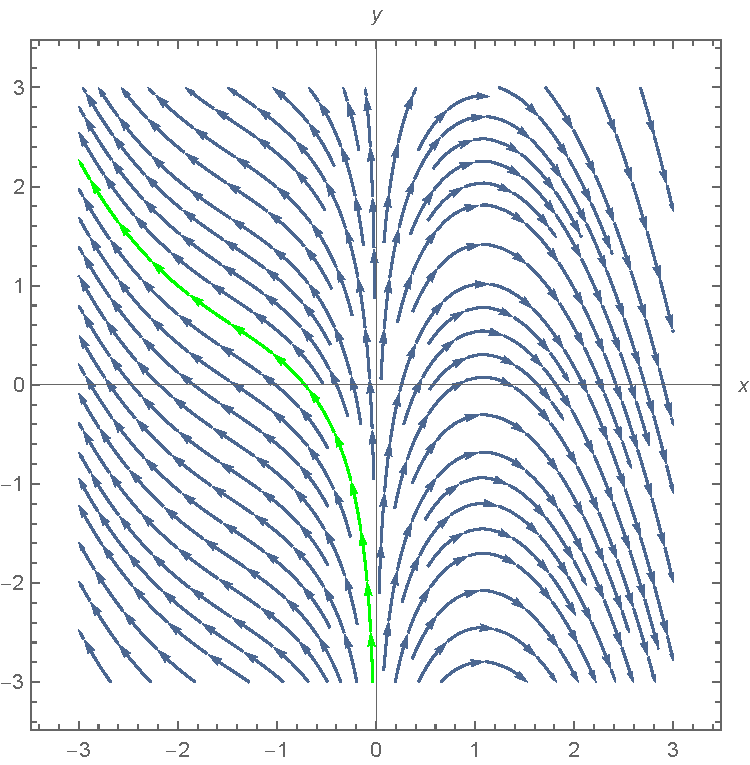
\includegraphics[width=\linewidth]{Images/integralcurve_1.pdf}
     \caption{the map $t \mapsto \theta_t(p)$ selects just one integral curve} \label{Fig:integralcurve_1}
\end{subfigure}
\begin{subfigure}{.45\textwidth}
     \centering
     \vspace{0.4em}
     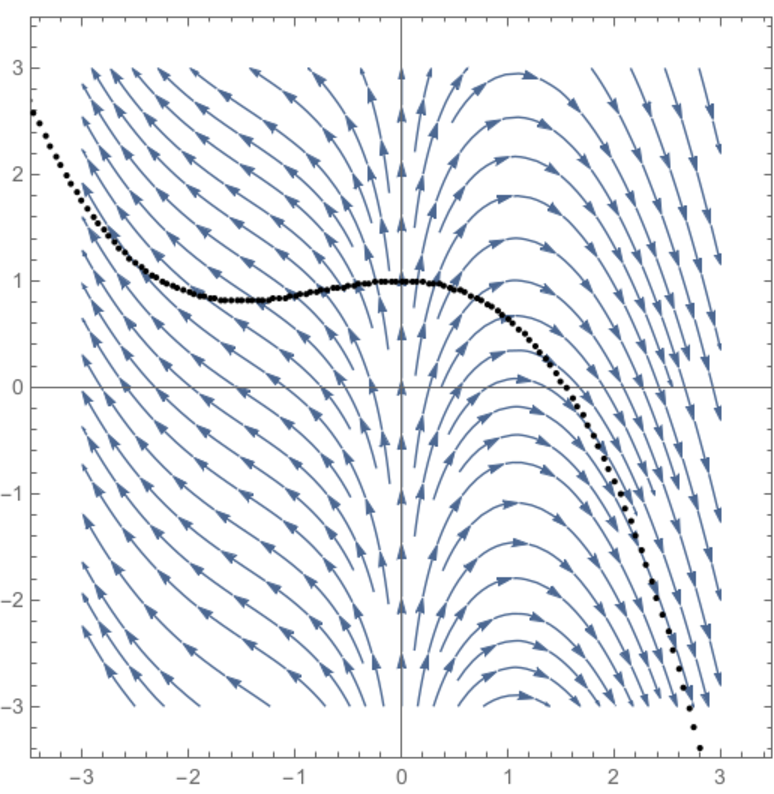
\includegraphics[width=0.95\linewidth]{Images/integralcurve_2.pdf}
     \caption{the map $p \mapsto \theta_t(p)$ selects all the curves evaluated at the same time $t$} \label{Fig:integralcurve_2}
\end{subfigure}
\end{figure}
\begin{itemize}
\item $p \mapsto \theta_t(p)$, for each fixed $t$ (we are observing several integral curves at the same time $t$),
\item $t \mapsto \theta_t(p)$, for each fixed $p$ (we are observing the integral curve starting from $p$, for all times).
\end{itemize}
\end{definition}

\begin{definition}[Lie derivative of a $k$-form]
  Let $z \in \mathfrak{X}(\rfield^n)$ be a differentiable vector field, $\phi_t$ its flow and $\omega \in \Omega^k(\rfield^n)$. Then the Lie derivative of $\omega$ is defined as
  \begin{equation}
    L_z \omega = \restrict{\frac{d}{dt}(\phi_t^* \omega)}{t=0} \, .
  \end{equation}
\end{definition}

\begin{remarkbox}\begin{remark}
  We denoted the flow by the symbol $\phi_t$ and not $\phi$. What we are doing here is not caring about $p$: $\phi^*_t \omega (\cdot) = \omega(\phi_t(\cdot))$.
  %In components we have: ...to do
  Useful formula (Cartan's formula): $L_z \omega = (d i_z + i_z d) \omega$.
\end{remark}\end{remarkbox}
\section[Lie Derivative of a Vector Field]{\crule[blue!50!white]{0.3cm}{0.4cm}  Lie Derivative of a Vector Field}
\begin{definition}[Pullback of a vector field through a diffeomorphism] \label{pulldiffeom}
  Let $\varphi$ be a diffeomorphism of $\rfield^n$ (i.e. a differentiable and invertible map from $\rfield^n$ to $\rfield^n$, such that its inverse is differentiable as well). Let $v \in \mathfrak{X}(\rfield^n)$. Then:
  \begin{equation}
    \varphi ^* v \equiv \varphi_* ^{-1}v
  \end{equation}
  is the pullback of $v$ with $\varphi$.
  In particular, given a flow $\phi$ and $t$ fixed, $\phi(t, \cdot) = \phi_t(\cdot)$ is a diffeomorphism on $\rfield^n$ with $\phi^{-1} = \phi(-t, \cdot) = \phi_{-t}(\cdot)$.
\end{definition}

\begin{definition}[Lie derivative of a vector field]
Let $u, v \in \mathfrak{X}(\rfield^n)$. Let $\phi$ be the flow of $u$. The Lie derivative of $v$ in direction $u$ is
\begin{equation}
  L_u v \equiv \restrict{\frac{d}{dt}( \phi_t^* v)}{t=0}
\end{equation}
(Remember: $\phi\colon (t, p) \mapsto \phi(t, p),$ whereas $ \phi^* v \colon (t, p) \mapsto v(\phi (t, p))$).
\end{definition}

\begin{lemma} \label{lemmadiff1}
  Let $u, v$ be smooth vector fields on $\rfield^n$ and $\varphi \in \Diff(\rfield^n)$. Let $\phi_t$ be the flow of $u$ and let $\psi_s$ be the flow of $v$. Then
  \begin{itemize}
    \item $\varphi^*v = \restrict{\frac{d}{ds}}{s=0} \varphi^{-1} \circ \psi_s \circ \varphi$,
    \item $\varphi^*v = v \Leftrightarrow \varphi \circ \psi_s = \psi_s \circ \varphi$ for all $s$,
    \item $L_u v = 0 \Leftrightarrow \phi_t \circ \psi_s = \psi_s \circ \phi_t$ for all $s, t$.
  \end{itemize}
\end{lemma}
\begin{proof}[Sketch of the proof]
$ $
\begin{itemize}
\item We have:
$$\restrict{\frac{d}{ds}}{s=0} \,  \varphi^{-1} \circ \psi_s \circ \varphi (p) \overset{(1)}{=} \varphi^{-1}_* (v_{\varphi(p)}) \overset{(2)}{=} (\varphi_*^{-1} v)_p \overset{(3)}{=} (\varphi^* v)_p$$
where we used: (1) the chain rule and the fact that $\psi_s$ is the flow of $v$. We applied the definitions to the point $\varphi(p)$ instead of $p$ as usual. (2) $(F_*X)_q = dF_{F^{-1}(q)}(X_{F^{-1}(q)})$, see also page 183 \citetalias{Lee}, (3) $\varphi_*^{-1} = \varphi^*$ by definition.
\item ($\Leftarrow$): if $\varphi \circ \psi_s = \psi_s \circ \varphi$ then, by using the previous point:
\[ \varphi^* v = \restrict{\deonde{s}}{s=0} \varphi^{-1} \circ \psi_s \circ \varphi = \restrict{\deonde{s}}{s=0} \psi_s = v \, . \]
($\Rightarrow$): if $\varphi^* v = v$, we use the previous point again:
\[ \restrict{\deonde{s}}{s=0} \psi_s = v = \restrict{\deonde{s}}{s=0} \varphi^{-1} \circ \psi_s \circ \varphi \, . \]
Now, the solution of such differential equation is unique because of the regularity assumptions on the flows. Then:
\[ \psi_s = \varphi^{-1} \circ \psi_s \circ \varphi \]
which implies the thesis.
\item $(\Leftarrow)$: follows from the previous point, and using the definition of Lie derivative for a vector field. $(\Rightarrow)$:
$$\frac{d}{dt} \phi_t^* v = \restrict{\frac{d}{d\varepsilon}}{\varepsilon=0} \phi^*_{t + \varepsilon} v \overset{(1)}{=} \phi_t^* \restrict{\frac{d}{d \varepsilon}}{\varepsilon=0} \phi^*_{\varepsilon} v = \phi_t^* L_u v = 0, \forall \, t$$
where in (1) we used that $\phi^*_{t + \varepsilon} = \phi_t^* \circ \phi^*_{\varepsilon}$.
Thus $\phi_t^* v = v \forall \, t$, and by the previous point we have the thesis. \qedhere
\end{itemize}
\end{proof}

\begin{lemma}
  Let $u, v$ be smooth vector fields on $\rfield^n$ and and let $\phi_t$ (respectively $\psi_s$) be the flow of $u$ (respectively $v$). Then:
  \begin{itemize}
    \item $L_u v = \restrict{\frac{\partial^2}{\partial s \partial t} \phi_{-t} \circ \psi_s \circ \phi_t}{t=0,s=0}$,
    \item $(L_u v) (f) = [u, v](f) = u(v(f)) - v(u(f))$ for all smooth functions $f$ on $\rfield^n$.
  \end{itemize}
\end{lemma}
\begin{proof}[Sketch of the proof]
$ $
\begin{itemize}
\item $\frac{d}{dt}\phi_t^* v = \frac{\partial}{\partial t} \frac{\partial}{\partial s} \phi_{-t} \circ \psi_s \circ \phi_t$ by the first point of the lemma \ref{lemmadiff1}, where we put $\varphi^* = \phi_t$.
\item See problem sheet 4, exercise 4. \qedhere
\end{itemize}
\end{proof}

\begin{lemma} \label{commlemma}
  Let $u, v$ be smooth vector fields on $\rfield^n$ and $\varphi \in \Diff(\rfield^n)$. Then:
  \begin{enumerate}
    \item $[u, v]$ is $\rfield-$bilinear (i.e. bilinear for a parameter $\lambda \in \rfield$),
    \item $[u, v] = - [v, u]$,
    \item The Jacobi identity holds,
    \item $[u, fv] = f[u, v] + u(f)v$,
    \item $\varphi_*[u, v] = [\varphi_* v, \varphi_* u]$.
  \end{enumerate}
\end{lemma}
\begin{proof}
See problem sheet 4, exercise 4.
\end{proof}

\begin{remarkbox} \begin{remark}[Naturality of the Lie bracket]
The property (5) of lemma \ref{commlemma} is called the \textbf{naturality} of the commutator. It implies that if $u, v$ are vector fields tangent to some space, then $[u, v]$ is tangent to the same space. See also problem sheet 12, ex. 3.
\end{remark} \end{remarkbox}

  \section[Stokes' Theorem on $\rfield^n$]{\crule[black!50!white]{0.3cm}{0.4cm}  Stokes' Theorem on $\rfield^n$}

\begin{itemize}
  \item For a function $f$ (i.e. a 0-form) on $[a, b] \subset \rfield$ we have $\int_a^b df = \int_a^b \partial_x f dx = f(b) - f(a)$ (fundamental theorem of calculus).
  \item for $\omega = a_i dx^i$, a 1-form on $U = [0, 1] \times [0, 1] \subset \rfield^2$ we have:
  $$\int_S d\omega = \int_S (\partial_{x^1} a_2) dx^1 \wedge dx^2 + (\partial_{x^2} a_1) dx^2 \wedge dx^1 = \int_{\partial S} \omega$$
  where we used the fundamental theorem of calculus.
  \item More generally, if $S$ is a compact subset of $\rfield^2$ with piecewise regular boundary $\partial S$ (piecewise homeomorphic to intervals in $\rfield$) then, by decomposing $S$ in terms of little squares and interpreting $\int_U d\omega$ as a Riemann sum over the square, we obtain the result
  $$\int_U d\omega = \int_{\partial U} \omega \, .$$
  This result generalizes immediately to compact co-dimension zero subsets of $\rfield^n$ with piecewise regulary boundary.
  \item If $M$ is a compact subset of dimension $m \le n$ in $\rfield^n$ (with piecewise regular boundary $\partial M$), diffeomorphic to a compact subset of $U \subset \rfield^m$ (i.e. $M = f(U)$) and $\omega \in \Omega^{m-1}(M)$, then:
  $$\int_M d\omega = \int_U f^* d\omega = \int_U df^* \omega = \int_{\partial U} f^* \omega = \int_{\partial M} \omega \, .$$
  \item More generally, the parametrization of $\partial M$ may be different from that induced by $M$. Then we have:
  $$\int_M d\omega = \int_{\partial M} i^* \omega$$
  where $i \colon \partial M \rightarrow M$ is the inclusion map of $\partial M$ into $M$.
\end{itemize}

So, the most general result that we achieved is the following:

\begin{theorem}[Stokes]
  Let $\omega \in \Omega^{m-1}(\rfield^n)$. Let $M$ be a compact subset of $\rfield^n$, $dim(M) = m \le n$, such that $M$ is homeomorphic to a closed subset $U \subset \rfield^m$. $\partial M$ is the boundary of $M$ and $i \colon \partial M \rightarrow M$ is the inclusion map of $\partial M$ into $M$. Then:
  \begin{equation}
    \int_{\partial M} i^* \omega = \int_M d\omega \, .
  \end{equation}
\end{theorem}
\begin{proof}[Sketch of the proof]
First, we notice that $U$ is compact as well because it is homeomorphic to a compact set.
Then, the proof uses the naturality of the pullback "$f^*d = df^*$" and the results for open subsets of $\rfield^n$.
\end{proof}

\begin{corollary}[Fundamental theorem of line integrals]
  Let $f$ be a smooth function defined near an oriented curve $C$ in $\rfield^n$, with endpoints $A$ and $B$.
  Then:
  \begin{equation}
    \int \nabla f \cdot dx = f(B)-f(A) \, . % TODO: add parametrization
  \end{equation}
\end{corollary}
\begin{proof}
	$\int df = \int \nabla f \cdot dx$ because $\nabla f \cdot dx = \frac{\partial f}{\partial x^i} dx^i = df$. Moreover, thanks to the Stokes' theorem, we have $\int df  = f(B) - f(A)$.
\end{proof}

\begin{corollary}[Curl theorem or Classical Stokes theorem]
  Let $v$ be a differentiable vector field defined near a surface $S \subset \rfield^3$ with boundary $\partial S$.
  \begin{equation}
    \int_S n \cdot (\nabla \times v) \, dS = \int_{\partial S} v \cdot dx
  \end{equation}
  where $n$ is the normal vector on the surface at each point.
\end{corollary}
\begin{proof}
Let $\alpha$ be a 1-form in $\rfield^3$. Since the Euclidean metric gives an isomorphism between $\rfield^3$ and its dual space (see also eq. \eqref{dualisomorph}), we can always write $\alpha$ as $\alpha = g(v, \cdot)$, for a certain $v \in \rfield^3$, where $g$ is the Euclidean metric, i.e. $g(x, y)$ is the standard dot product between $x$ and $y$. So, $\alpha = g(v, \cdot) = \delta_{ij} v^j dx^i = v_i dx^i$ in the dual basis $\{dx^i\}$. Then: $d \alpha = (\partial_{x^j} v_i) dx^j \wedge dx^i \overset{(1)}{=} \partial_{x^j} v_i \varepsilon^{ji}_k n^k dS$. Where in (1) we used that $dx^j \wedge dx^i$ is the oriented surface generated by $dx^j$ and $dx^i$ (see also the second point of the example \ref{orarea}). Then we used that the oriented surface area can be expressed using the Levi-Civita tensor $\varepsilon$, the normal vector $n$ and the unoriented area element $dS$. Hence, using that $\nabla \times v = \partial_{x^j} v_i \varepsilon^{ji}_k$:
$$\int_S n \cdot (\nabla \times v) \, dS = \int_S d\alpha \overset{(2)}{=} \int_{\partial S} \alpha = \int_{\partial S} v_i dx^i = \int_{\partial S} v \cdot dx$$
using the Stokes' theorem in (2).
\end{proof}

\begin{corollary}[Divergence theorem]
  For a smooth vector field $v$ defined on a solid $T \subset \rfield^3$ with boundary $\partial T$:
  \begin{equation}
    \int_T \nabla \cdot v \, dV = \int_{\partial T} v \cdot n \, dS
  \end{equation}
  where $dV$ is the unoriented volume element.
\end{corollary}
\begin{proof}
See problem sheet 5, exercise 3.
\end{proof}

\section[Closed and Exact $k$-forms]{\crule[brown!50!white]{0.3cm}{0.4cm}  Closed and Exact $k$-forms}
\begin{definition} [Closed and exact forms]
  If $\omega \in \Omega^{k}(U)$ such that $d\omega = 0$, then $\omega$ is closed. If there exists $\alpha \in \Omega ^{k-1}(V), V \subset U$ such that $\omega = d\alpha$ in $V$ then $\omega$ is exact.
\end{definition}

\begin{proposition} \label{propex1forms}
  The following are equivalent (\textbf{note that we are considering just 1-forms!}):
  \begin{enumerate}
    \item $\omega \in \Omega^1(U)$ is exact in a connected open subset $V \subset U$,
    \item For any curve $\gamma \colon (a, b) \rightarrow U, \int_{\gamma} \omega$ depends only on the endpoints $\gamma(a)$ and $\gamma(b)$,
    \item $\int_{\gamma} \omega = 0$ for any closed curve $\gamma$ in $V$.
  \end{enumerate}
\end{proposition}
\begin{proof}[Sketch of the proof]
First, $(1) \Rightarrow (2)$ because of Stokes' theorem. Moreover, $(2) \Rightarrow (3)$ using Stokes' theorem again. Now, $(3) \Rightarrow (2):$ the curve made of the union of $\gamma_1$ and $\gamma_2$ is a closed curve. Then, if $\gamma$ is the name of such a closed curve:
$$0 = \int_{\gamma} \omega = \int_{\gamma_1} \omega - \int_{\gamma_2} \omega$$
where the minus sign comes from the orientation of the curves.
Then: $\int_{\gamma_1} \omega = \int_{\gamma_2} \omega$ where $\gamma_1$ and $\gamma_2$ are any two curves with the same endpoints. It means that we can consider the integral of $\omega$ on any curve and the result  wouldn't change, \textbf{if} the new curve has the same endpoints of the initial curve.
\begin{figure}[H] \label{Fig:closedcurve}
     \centering
     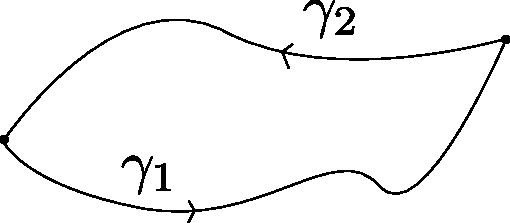
\includegraphics[width=0.3\textwidth]{Images/closedcurve.pdf}
     \caption{Union of $\gamma_1$ and $\gamma_2$}
\end{figure}
$(2) \Rightarrow (1)$: Let's consider the 1-form $\omega = a_i dx^i$ (when $\omega$ has this form, we call it a \textit{standard form}). Let's fix a point $p \in V$ and define a function
\begin{align*}
f \colon V &\rightarrow \rfield \\
x &\mapsto \int_{\gamma} \omega
\end{align*}
where $x = x(p')$ is the coordinate given by a point $p'$ (i.e. $x$ gives a parametrization) and $\gamma$ is a curve joining $p$ to $p'$. By (2), $f$ is well defined (i.e. the definition does not depend on the $\gamma$ chosen, so we don't need to specify it). Furthermore, $df = \frac{\partial f}{\partial x^i} dx^i$. Since $\omega = a_i dx^i$, we only need  to prove that $\frac{\partial f}{\partial x^i} = a_i$. Let's consider the curve $\gamma$. We extend it from $p'$ with a straight segment $\Delta \gamma$. In particular, $\Delta \gamma = x + t e_i, t \in (-\varepsilon, \varepsilon)$ with $e_i$ any vector of the canonical basis of $\rfield^n$. We choose $\varepsilon$ small such that $\gamma + \Delta \gamma \subset V$. Then:
\begin{align*}
\restrict{\frac{\partial f}{\partial x^i}}{x} &= \lim\limits_{t \to 0} \frac{1}{t} \left[ f(x+t e_i) - f(x) \right] = \lim\limits_{t \to 0} \frac{1}{t} \left[  \int_{\gamma + \Delta \gamma} \omega - \int_{\gamma} \omega \right] = \\
&= \lim\limits_{t \to 0} \frac{1}{t} \int_{\Delta \gamma} \omega = \lim\limits_{t \to 0} \frac{1}{t} \int_0^t a_i(x(t)) dt = a_i(x)
\end{align*}
where we used $\int \omega = \int a_i \frac{dx^i}{dt} dt$ and the fact that every point belonging to $\Delta \gamma$ can be written as $x + t e_i$, so we have $\frac{dx^i}{dt} = 1$ on $\Delta \gamma$. Moreover, in the last equality we Taylor-expanded $a_i(x(t))$ with respect to $t$. Only the first-order term $a_i(x)$ matters because we are considering the limit as $t \to 0$. Then we have the thesis for standard forms. Then, the result holds for any form (in general we could have $a_i = 0$ for some $i$).
\begin{figure}[H] \label{Fig:pcurve}
     \centering
     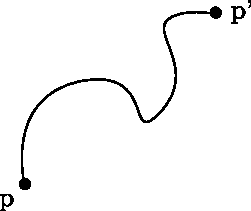
\includegraphics[width=0.24\textwidth]{Images/pp'.pdf}
     \caption{A possible curve $\gamma$ from $p$ to $p'$} \qedhere
\end{figure} 
\end{proof}

\begin{remarkbox}\begin{remark}[A closed form is not always exact]
  If $\omega$ is exact, then it is closed (because $d^2=0$). But not every closed form in $\Omega^1(U), U$ open subset of $\rfield^n$ is exact. Cf. $\omega = - \frac{y}{x^2 + y^2} dx + \frac{x}{x^2+y^2}dy$ in $\rfield^2$ minus the non-negative $x$-axis. If $\gamma$ is a closed curve around the origin of $\rfield^2$, we have:
  $$\int_{\gamma} \omega = \int_{\gamma} d\theta = 2\pi$$
  and therefore $\omega$ cannot be exact by the previous proposition. However, we notice that we have problems only with the origin of $\rfield^2$. If we consider a subset of $\rfield^2$ which is far enough from the origin, the form would be an exact form in such subset. Indeed, we say that $\omega$ is locally exact, and the general result follows from the next theorem.
\end{remark}\end{remarkbox}

\begin{theorem}[Poincarè theorem for 1-forms on $\rfield^n$]
  Let $\omega \in \Omega^1(U), U \subset \rfield^n, U$ open. Then $d\omega = 0$ if and only if for each $p \in U$ there is a neighbourhood $V \subset U$ of $p$ and a differentiable function $f \colon V \rightarrow \rfield$ such that $\omega = df$.
\end{theorem}

\begin{remarkbox}\begin{remark}
  We will not prove this theorem, because it follows from the more general case for $k$-forms, that we will analyze in the next pages.
  Using the Poincarè theorem for 1-forms, we can extend the definition of the integral of a closed 1-form along a \textbf{continuous} path (until now, we have always assumed the our paths were piecewise differentiable). In fact, assume that $ \omega \in \Omega^1(U), d \omega = 0$, and $\gamma$ such that:
  $$\gamma \colon [0, 1] \rightarrow U$$ is a differentiable map.
  Now, we choose a partition of $[0, 1]$, i.e. a collection of points $0 = t_0 < t_1 < \ldots < t_k < t_{k+1} = 1$ such that the restriction of $\gamma$ to the interval $(t_i, t_{i+1})$ is contained in a ball $B_i$ where $\omega$ is exact. In particular:
  $$\omega = df_i, \text{ for } f_i \colon B_i \rightarrow \rfield \, .$$
  Then:
  $$\int_{\gamma} \omega = \sum_i \left[ f_i(t_{i+1}) - f_i(t_i) \right ] \, .$$
  If $\gamma$ is only continuous, we could still consider such a partition, and still define
  $$\int_{\gamma} \omega = \sum_i \left[ f_i(t_{i+1}) - f_i(t_i) \right ] \, .$$
  The integral of $\gamma$ is well defined because the definition is independent from the choice of our partition: if $P$ is one partition and $P'$ is a refinement of $P$ (i.e. it is the same partition plus an extra point $t' \in (t_i, t_{i+1})$ for some $i$), then:
  $$[f_i(t_{i+1}) - \cancel{f_i(t')}] + [\cancel{f_i(t')} - f_i(t_i)] = [f_i(t_{i+1}) - f_i(t_i)] \, .$$
  Then the integral does not change if we consider a refinement. If we consider a general partition $P'$, we can add every point of the partition $P$ to $P'$, so that we get a refinement of $P'$ that we will call $P''$. The integral on the partition $P'$ has the same value of the integral on the partition $P''$ by the above argument. Now, we can add every point of the partition $P'$ to $P$, so to get the partition $P''$ again, but now we can see $P''$ as a refinement of $P$. Then the integral on $P$ and on $P''$ are the same. Then also the integrals on $P$ and $P'$ are the same.
\end{remark}\end{remarkbox}

Now, we want to extend the above theorem to $k$-forms.

\begin{definition} [Contractible set]
  An open subset $U \subset \rfield^n$ is contractible to some point $p_0 \in U$ if there exists a differentiable map
  \begin{align}
    H \colon U \times [0, 1] &\rightarrow U \\
    (p,t) &\mapsto H(p, t) \nonumber
  \end{align}
  such that $H(p, 1) = p, H(p, 0) = p_0, \forall\, p \in U$.
\end{definition}

\begin{tcolorbox}\begin{example}
$\rfield^n$ is contractible to any point $p_0 \in \rfield^n$. The homotopy is given by:
$$H(p, t) = p_0 + t(p- p_0) \, .$$
\end{example}\end{tcolorbox}

\begin{remarkbox}\begin{remark}
  If $U$ is contractible, we can associate a $k$-form $\bar\omega \in \Omega^k(U \times \rfield)$ to every $\omega \in \Omega^k(U)$. $\bar \omega$ is defined as
  \begin{equation}
    \bar\omega = H^* \omega \, .
  \end{equation}
  Conversely, we can associate a $k$-form $\omega \in \Omega^k(U)$ to each $\bar \omega \in \Omega^k(U \times \rfield)$ with the help of the inclusion map
  \begin{align}
    i_t \colon U &\rightarrow U \times \rfield \\
    p &\mapsto i_t(p) = (p,t)\nonumber
  \end{align}
  Then, $i_t^* \bar \omega \in \Omega^k(U)$ if $\bar \omega \in \Omega^k(U \times \rfield)$.
 \end{remark}\end{remarkbox}

 \begin{lemma}   \label{lemmaform1}
  Any $k$-form on $U \times \rfield$ has a unique decomposition of the form
  \begin{equation}
    \bar \omega = \omega_1 + dt \wedge \eta
  \end{equation}
  where $\omega_1 \in \Omega^k(U \times \rfield), \eta \in \Omega^{k-1}(U \times \rfield)$, and with $i_{\partial_t} \omega_1 = 0$ and $i_{\partial_t} \eta = 0$.
  \end{lemma}


\begin{proof}
  Let's choose coordinates $\{x^1, \ldots, x^n, t\}$ for $U \times \rfield$. Then we write $\bar \omega$ on the basis:
  $$\bar \omega = \sum\limits_{i_1 < \ldots < i_k} a_{i_1 \cdots i_k} dx^{i_1} \wedge \ldots \wedge dx^{i_k} + \sum_{i_1 < \ldots < i_{k-1}} b_{i_1 \ldots i_{k-1}} dt \wedge dx^{i_1} \wedge \ldots \wedge dx^{i_{k-1}} \, .$$
  (We can always do this, the coefficients could also be trivial). Obviously, we have $i_{\partial_t} \omega_1 = 0$ and $i_{\partial_t} \eta = 0$ by definition of dual basis: $dx^{j} (\partial_t) = 0, \forall \, j$, $dt(\partial_t) = 1$.
\end{proof}

\begin{remarkbox} \begin{remark} \label{intremark}
Now, we want to integrate the form $\bar \omega = \omega_1 + dt \wedge \eta$ of lemma \ref{lemmaform1}.
Let's define the map
  \begin{align}
    I \colon \Omega^k(U \times \rfield) &\rightarrow \Omega^{k-1}(U) \\
    \eta &\mapsto I\eta \nonumber
  \end{align}
  such that $$(I\eta)(z_1, \ldots, z_{k-1}) = \int_0^1 \eta(p, t)(\partial_t, i_{t}^*z_1, \ldots, i_{t}^*z_{k-1})dt$$
where we used the inclusion map:
  \begin{align} \label{definclusion}
    i_t \colon U &\rightarrow U \times \rfield \\
    p &\mapsto (p, t) \nonumber
  \end{align}
  and here $i_t$ "includes" $U$ into $U \times \rfield$ at $t$ (it is \textbf{not} the interior derivative!)
\end{remark}\end{remarkbox}

\begin{lemma} \label{lemmaform2}
The following holds:
  \begin{equation}
    i_1^* \bar \omega - i_0^* \bar \omega = d(I \bar \omega) + I(d\bar \omega)
  \end{equation}
  where $i_1$ is $i_t$ for $t=1$, and $I$ is the integration defined in remark \ref{intremark}. $i^*_t\colon \Omega(U \times \rfield \rightarrow \Omega(U)$ is the pullback of $i_t$.
\end{lemma}
\begin{proof}
%Indeed, since $H \circ i_1 = Id$ and $H \circ i_0 = p_0$, $\forall \, p \in U$ we have
  %$$\omega = (H \circ i_1)^* \omega = i_1^* \bar \omega$$
  %and
  %$$0 = (H \circ i_0)^* \omega = i_0^* \bar \omega$$
  Let's consider $p \in U$ with coordinates $x^1, \ldots, x^n$. Since everything is linear, we just need to check the thesis for the single terms in the sum $\bar \omega = \omega_1 + dt \wedge \eta$.
  \begin{description}
  \item[case a)] Assume:
  \begin{equation} \label{omegacasea}
  \bar \omega = f \, dx^{i_1} \wedge \ldots \wedge dx^{i_k}
  \end{equation}
  Then:
  \begin{align*}
  d \bar \omega = df \wedge dx^{i_1} \wedge \ldots \wedge dx^{i_k} = \defonde{f}{t} dt \wedge dx^{i_1} \wedge \ldots \wedge dx^{i_k} + \defonde{f}{x^i} dx^i \wedge dx^{i_1} \wedge \ldots \wedge dx^{i_k} \, .
  \end{align*}
  So:
  $$I(d\bar \omega) = \int_0^1 \defonde{f}{t}(p, t) \underbrace{i_t^* dx^{i_1}}_{=dx^{i_1}} \wedge \ldots \wedge i_t^* dx^{i_k} dt = (f(p, 1) - f(p, 0)) dx^{i_1} \wedge \ldots \wedge dx^{i_k} = i_1^* \bar \omega - i_0^* \bar \omega \, .$$
  Moreover, $I\bar \omega = 0$ because $\bar \omega$ (cf. \eqref{omegacasea}) does not contain any $dt$ in this case.
  \item[case b)] Assume:
  \begin{equation} \label{omegacaseb}
  \bar \omega  = f\, dt \wedge dx^{i_1} \wedge \ldots  \wedge dx^{i_{k-1}} \, .
  \end{equation}
  Then:
  $$d \bar \omega = \defonde{f}{x^i} dx^i \wedge dt \wedge dx^{i_1} \wedge \ldots  \wedge dx^{i_{k-1}} \, .$$
  So, changing the order of the basis and getting a minus sign:
  $$I(d \bar \omega) = - \int_0^1 \defonde{f}{x^i} dx^i \wedge dx^{i_1} \wedge \ldots \wedge dx^{i_{k-1}} dt \, .$$
  And also:
  $$d(I \bar \omega) = d \int_0^1 f(p, t) dx^{i_1} \wedge \ldots \wedge dx^{i_{k-1}} dt = \int_0^1 \defonde{f}{x^i} dx^i \wedge dx^{i_1} \wedge \ldots \wedge dx^{i_{k-1}} dt \, .$$
  Thus, we have $I(d \bar \omega) + d(I \bar \omega) = 0$. In this case (cf. \eqref{omegacaseb}), we also have $i_t^* dt = 0$ (recall that $i_t \colon p \mapsto (p, t)$). Therefore: $i_t^* \bar \omega = 0, \forall \, t$. \qedhere
  \end{description}





\end{proof}

Then we can extend Poincarè lemma to $k$-forms:
\begin{theorem} [Poincarè Lemma] \label{poinclemma}
  Let $k \ge 1$. Let $U$ be a contractible, open subset of $\rfield^n$ and $\omega \in \Omega^k(U)$ with $d\omega = 0$. Then there exists a $(k-1)$-form $\alpha \in \Omega^{k-1} (U)$ such that $\omega = d\alpha$.
\end{theorem}
\begin{proof}
The proof follows from the previous lemmas  \ref{lemmaform1} and \ref{lemmaform2}. In fact, in the hypotheses of the theorem, the $\alpha$ that we need is $\alpha = I \bar \omega$. Indeed: given $\omega \in \Omega^k(U)$, we can define $\bar \omega = H^* \omega \in \Omega^k(U \times \rfield)$, where $H$ is the map that can contract $U$ to a point. If we consider the map $i_t$ defined in \eqref{definclusion}, we have:
$$H \circ i_1 = \id \quad \text{and} \quad H \circ i_0 = \text{const.}$$
So:
$$\omega = (H \circ i_1)^* \omega = i_1^* (H^* \omega) = i_1^* \bar \omega$$
and by remark \ref{effectivepullback} we know that the pullback of a $k-$form ($k \ge 1$) through a constant map is 0, so we also have:
$$0 = (H \circ i_0)^* \omega = i_0^* (H^* \omega) = i_0^* \bar \omega \, .$$
From the lemma \ref{lemmaform2}, we know that $i_1^* \bar \omega - i_0^* \bar \omega = d(I \bar \omega) + I(d \bar \omega) $. From previous computations, it means:
$$\omega = d(I \bar \omega) + I (d \bar \omega) \, .$$
Actually, $I (d \bar \omega) = 0$ because $d \bar \omega = 0$. Indeed:
$$d \bar \omega = d(H^* \omega) \overset{(1)}{=} H^* d \omega \overset{(2)}{=} 0$$
where we used: (1) naturality of the pullback, cf. proposition \ref{pullbackprop}, point 5, (2) $d \omega = 0$ by assumption.
Then, $\omega = d(I \bar \omega)$.
\end{proof}

Question: For $\omega \in \Omega^1(U)$, when is $\int_{\gamma}\omega$ independent of the choice of $\gamma$?

\begin{definition}[Homotopy between curves]
  Two continuous curves $\gamma_1$ and $\gamma_2$, $\gamma_i \colon [a, b] \rightarrow U, i=1,2, U \subset \rfield^n$ are freely homotopic if there exists a continuous map $H$
  \begin{align*}
    H \colon [a, b] &\times [0, 1] \rightarrow U &\text{ such that:}\\
    H(s, 0) &= \gamma_1(s), &\forall\, s \in [a, b] \\
    H(s, 1) &= \gamma_2(s), &\forall\, s \in [a, b]
  \end{align*}
  \begin{figure}[H] \label{Fig:hom1}
     \centering
     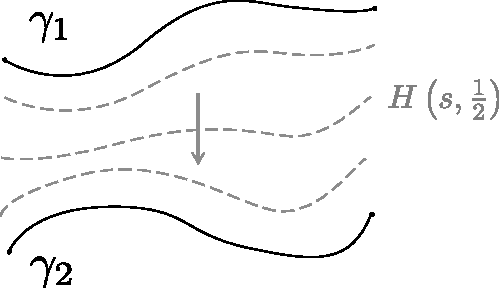
\includegraphics[width=0.4\textwidth]{Images/homotopy1.pdf}
     \caption{Homotopy between curves}
\end{figure}
\end{definition}

\begin{definition}[Homotopy between curves with same endpoints]
  Two continuous curves $\gamma_1$ and $\gamma_2$, $\gamma_i \colon [a, b] \rightarrow U, i=1,2, U \subset \rfield^n$, with $\gamma_1(a) = \gamma_2(a)$ and $\gamma_1(b) = \gamma_2(b)$ are homotopic relatively to $\{\gamma_1(a), \gamma_2(b)\}$ if there exists a continuous map $H$
  \begin{align*}
    H \colon [a, b] &\times [0, 1] \rightarrow U &\text{ such that:}\\
    H(s, 0) &= \gamma_1(s), &\forall\, s \in [a, b] \\
    H(s, 1) &= \gamma_2(s), &\forall\, s \in [a, b] \\
    H(a, t) &= \gamma_1(a) = \gamma_2(a), &\forall\, t \in [0, 1] \\
    H(b, t) &= \gamma_1(b) = \gamma_2(b), &\forall\, t \in [0, 1]
  \end{align*}
  \begin{figure}[H] \label{Fig:hom2}
     \centering
     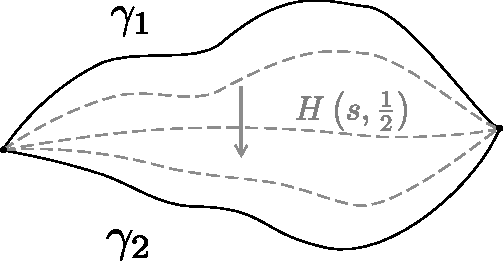
\includegraphics[width=0.4\textwidth]{Images/homotopy2.pdf}
     \caption{Homotopy between curves with same endpoints}
\end{figure}
\end{definition}

\begin{theorem}
  Let $\omega \in \Omega^1(U)$, with $d \omega = 0$ (closed), and $\gamma_1, \gamma_2$ be two homotopic curves with same endpoints. then:
  \begin{equation}
    \int_{\gamma_1} \omega = \int_{\gamma_2} \omega \, .
  \end{equation}
\end{theorem}
\begin{proof}
Let's suppose the two curves do not intersect each other.
We can go through $\gamma_1$ backwards. Let $I$ be the interior of the space bounded by the two curves.
\begin{figure}[H] \label{Fig:hom4}
     \centering
     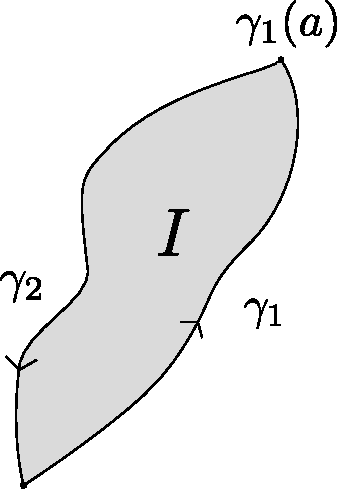
\includegraphics[width=0.18\textwidth]{Images/homotopy4.pdf}
\end{figure}
$I$ is contractible, then by Poincarè lemma \ref{poinclemma}, $\omega$ is exact in $I$. Using Stokes's theorem and denoting the curve $\gamma_1$ with reversed orientation by $\hat \gamma_1$:
$$\int_{\hat \gamma_1 + \gamma_2} \omega = \int_I d \omega = 0$$
where last equality follows from the exactness of $\omega$: $d\omega = d^2 \alpha=0$ for some 0-form $\alpha$.
On the other hand, if the two curves intersect each other, we split the curves for each intersection and apply the previous proof for each one of them.
\end{proof}

What if $\gamma_1(a) \not = \gamma_2(a), \gamma_1(b) \not = \gamma_2(b)$?
\begin{definition}[Homotopy between closed curves]
$\gamma_1, \gamma_2 \colon [a, b] \rightarrow U$, $\gamma_i$ closed curves, are freely homotopic if there exists a continuous map
\begin{align*}
  H \colon [a, b] \times [0, 1] &\rightarrow U &\text{ such that:} \\
  H(s, 0) &= \gamma_1(s), &\forall\, s \in [a, b] \\
  H(s, 1) &= \gamma_2(s), &\forall\, s \in [a, b] \\
  H(a, t) &= H(b, t), &\forall\, t \in [0, 1]
\end{align*}
 \begin{figure}[H] \label{Fig:hom3}
     \centering
     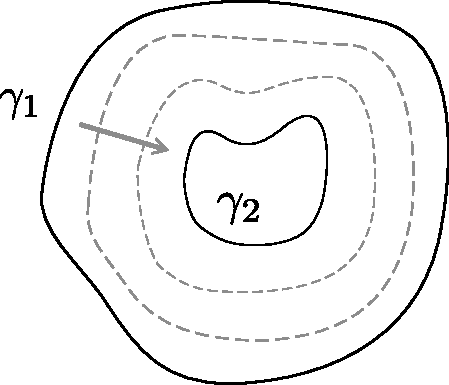
\includegraphics[width=0.3\textwidth]{Images/homotopy3.pdf}
     \caption{Homotopy between closed curves}
\end{figure}
\end{definition}

\begin{proposition}
  If $\omega$ is a closed 1-form on $U$, $\gamma_1$ and $\gamma_2$ two closed curves, freely homotopic in $U$, then:
  \begin{equation}
    \int_{\gamma_1} \omega = \int_{\gamma_2} \omega \, .
  \end{equation}
  In particular, if $\gamma_1$ is freely homotopic to a point, then $\int_{\gamma_1} \omega = 0$
\end{proposition}
\begin{proof}[Idea of the proof]
We can decompose the space in small squares and use the Stokes' theorem for each of them.
\end{proof}

\begin{definition}[Simply connected set] \label{closedinsimplyconn}
  %\marginpar{If $U$ is arc-wise connected we also say that it is simply connected if its fundamental group is trivial}
  A connected open set $U \subset \rfield^n$ is simply connected if every continuous closed curve in $U$ is freely homotopic to a point in $U$.
\end{definition}

\begin{tcolorbox}\begin{example}
  $\rfield^n$, the unitary ball in $\rfield^n$ and its homeomorphic images are simply connected.
\end{example}\end{tcolorbox}

\begin{remarkbox}\begin{remark}[Contractible vs. simply connected]
"Contractible $\Longrightarrow$ simply connected" (every single point of a closed curve can be brought to a point), but "simply connected $\cancel{\Longrightarrow}$ contractible" (cf. $S^2$, from intuition we can say that contracting the sphere to a point implies "cutting" the sphere somewhere, and it can't be done in a continuous way).
\end{remark}\end{remarkbox}

\begin{remarkbox}\begin{remark}
  Every closed 1-form on a simply connected subset $U$ of $\rfield^n$ is exact. Indeed, $\int_{\gamma} \omega = 0$ for every closed $\gamma$ in the space, where $\omega$ is a closed 1-form, because every closed curve can be shrinked to a point (by def. \ref{closedinsimplyconn}). By proposition \ref{propex1forms}, $\omega$ is exact. The result is not true for $k$-forms (in such cases, we need more advanced tools).
\end{remark}\end{remarkbox}

We can limit ourselves to consider continuous curves, thanks to the two following results:
\begin{theorem}[Whitney approximation on $\rfield^n$] \label{whitney}
  If $\gamma$ is a continuous map between $U, V \subsetneq \rfield^n$, then $\gamma$ is homotopic to a smooth map $\tilde \gamma$. If $\gamma$ is smooth on a closed subset $A$ of $U$, then the homotopy can be taken relatively to $A$.
\end{theorem}

\begin{theorem}
  If $\gamma_1$ and $\gamma_2$ are homotopic maps between $U$ and $V$ then they are smoothly homotopic. %TO CHECK
\end{theorem}
\section[De Rham Cohomology]{\crule[green!50!white]{0.3cm}{0.4cm}  De Rham Cohomology}


Let $U$ be an open subset of $\rfield^n$. We can think of $\Omega^k(U)$ as a vector space over $\rfield$. Indeed, if $\alpha, \beta \in \Omega^k(U)$, then $a \alpha + b \beta \in \Omega^k(U), \forall\, a, b, \in \rfield$. Also the remaining properties of a vector space are satisfied.

\begin{remarkbox}\begin{remark}
  We say that $\Omega^k(U, \mathbb{Z}) = \{k\text{-forms on } U \text{ with coefficients in } \mathbb{Z}\}$  forms a group (and not a vector space) since $\mathbb{Z}$ is not a field. In contrast, $\Omega^k(U, \rfield)$ is a vector space. We will often denote $\Omega^k(U, \rfield)$ just by $\Omega^k(U)$.
\end{remark}\end{remarkbox}

Now, we want to introduce some concepts of cohomology theory (see also page 460, \citetalias{Lee}).

\begin{definition}[Complex]
Let $\mathcal{R}$ be a commutative ring (let's suppose $\mathcal{R} = \rfield$ because it is the case we are interested in). Let's consider the sequence
\[ \cdots  \longrightarrow A^{k-1} \overset{d}{\longrightarrow} A^k \overset{d}{\longrightarrow}A^{k+1} \longrightarrow \cdots \]
where for every $k$, $A^k$ is a vector space on $\rfield$ and the maps $d$ are linear maps. Such a sequence is said to be a complex if the composition of any two successive applications of $d$ is the zero map:
\[ d \circ d = 0 \colon A^k \rightarrow A^{k+2} \text{ for each } k\, . \]
Sometimes it is also called a cochain complex, whereas it is called a chain complex if the arrows go in the opposite direction.
Sometimes we use the notation $d_k \colon A^{k-1} \rightarrow A^k$ to denote the position of the map in the sequence.
It's easy to see that such a definition implies that $\im(d_k) \subset \ker(d_{k+1})$.
\end{definition}

\begin{definition}[Exact sequence]
Let $A^*$ be a complex. It is called an exact sequence if $\im(d_k) = \ker(d_{k+1})$.
\end{definition}

\begin{definition}[K-th cohomology group]
Let $A^*$ be a complex. We define the k-th cohomology group of $A^*$ to be the quotient module
\[H^k(A^*) \equiv \faktor{\ker(d_{k+1})}{\im(d_k)}\, . \]
It is well defined since $\im(d_k) \subset \ker(d_{k+1})$ by definition of cochain complex. If we are dealing with a chain complex, it is called homology group instead of cohomology group. The linear map $d$ can be any map, but when $d$ is the exterior derivative and the complex is given by a sequence of the vector spaces $\Omega^k(U)$, the cohomology group gives us information about the failure of exactness at $\Omega^k(U)$ (it is an information about the space, not about the forms).
\end{definition}

\begin{definition}[de Rham complex]
  The de Rham complex is the sequence
  $$\cdots \overset{d}{\longrightarrow} \Omega^{k-1} \overset{d}{\longrightarrow} \Omega^{k} \overset{d}{\longrightarrow} \Omega^{k+1} \overset{d}{\longrightarrow} \cdots \overset{d}{\longrightarrow} \Omega^{n} \overset{d}{\longrightarrow} 0 $$
  where $d$ is the exterior derivative now. It is well defined since we know that $d^2 = d \circ d = 0$ from the properties of the exterior derivative. Thus, $\im(d_k) \subset \ker(d_{k+1})$. Notice that we wrote $\Omega^k$ instead of $\Omega^k(U)$ for the sake of simplicity, and that the sequence stops at $\Omega^n$ because $U \subset \rfield^n$.
\end{definition}

\begin{definition}[de Rham cohomology group] \label{drremark}
  Let $U \subset \rfield^n$, $U$ open, $\dim(U) = m \le n$. Then:
  \begin{itemize}
    \item The set of closed $k$-forms is the $k$-th \textit{cocycle group} $Z^k(U, \rfield)$ (it is a group with respect to addition),
    \item The set of exact $k$-forms is the $k$-th \textit{coboundary group} $B^k(U, \rfield)$,
    \item The $k$-th \textit{de Rham cohomology group} $H^k(U, \rfield)$ is defined as: $$H^k(U, \rfield) \equiv \faktor{Z^k(U, \rfield)}{B^k(U, \rfield)} = \faktor{\ker(d_{k+1})}{\im(d_k)} \, .$$
  \end{itemize}
\end{definition}

\begin{remarkbox}\begin{remark}[Cohomologous forms]
  $H^k(U, \rfield)$ contains the closed $k$-forms defined on $U$ which are not exact. Indeed, remember the definition of $d_k\colon \Omega^{k-1} \rightarrow \Omega^k $. The set $\ker(d_{k+1})$ contains all the $k$ forms that are closed. The set $\im(d_k)$ contains the exact forms. As usual when we deal with vector spaces, the equivalence relation is:
  \begin{equation} \label{cohomol}
  \omega \sim \omega' \Leftrightarrow \omega - \omega' \in \im(d_k) \Leftrightarrow \omega - \omega' = d\alpha \text{ for some (} k-1 \text{)-form } \alpha \, .
  \end{equation}
  From the above definition, we see that two closed forms $\omega, \omega'$ are in the same equivalence class (so they are said to be \textbf{cohomologous}) if they differ by an exact form.
  Obviously, if $\omega$ and $\omega'$ are exact, we have $\omega = dF$ and $\omega'=dG$ for some ($k-1$)-forms $F$ and $G$. So, the two forms are cohomologous because the $\alpha$ that we need in the definition \eqref{cohomol} is $\alpha = F - G$. All the exact forms are identified with the 0 element of $H^k(U, \rfield)$, because $\omega \sim 0$ if $\omega$ is an exact ($k-1$)-form (the difference between $\omega$ and 0 is an exact form).
  To read more about quotient spaces, see also the example \ref{quotientexample}.
\end{remark}\end{remarkbox}

\begin{tcolorbox}\begin{example}
  Let's consider the following examples:
  \begin{itemize}
    \item If $U$ is contractible, then $H^k(U, \rfield) = \{0\}$ by Poincarè lemma,
    \item $U=\rfield^2 \setminus \{0\}$, $H^0(\rfield^2 \setminus \{0\}, \rfield) = \rfield$ (constant functions),
    \item $H^1(\rfield^2 \setminus \{0\}, \rfield) = \rfield$,
    \item $H^2(\rfield^2 \setminus \{0\}, \rfield) = \{0\}$,
    \item Torus $T$: $H^0(T) = \rfield$,  $H^1(T) = \rfield \oplus \rfield$, $H^2(T) = \rfield$.
  \end{itemize}
\end{example}\end{tcolorbox}

\begin{definition}
  If $M \subset \rfield^n$, then we define:
  \[  \Omega^*(M, \rfield) \equiv \bigoplus_{k=0}^n \Omega^k(M, \rfield) \, . \]
\end{definition}

\begin{remarkbox}\begin{remark}
  $\wedge \colon \Omega^* \times \Omega^* \rightarrow \Omega^*$ endows $\Omega^*$ with the structure of a ring.
\end{remark}\end{remarkbox}

\begin{remarkbox}\begin{remark} [Exact sequence] \label{exsequence}
  If $H^k(M, \rfield) = 0$ for $k=1, \ldots, n$, then
    $$\cdots \overset{d}{\longrightarrow} \Omega^{k-1} \overset{d}{\longrightarrow} \Omega^{k} \overset{d}{\longrightarrow} \Omega^{k+1} \overset{d}{\longrightarrow} \cdots $$
    is an exact sequence because every closed form is exact, so $\ker(d_{k+1}) = \im(d_k)$. Notice that for $k=0$, $\Omega^0 = \{\text{functions}\}$, then $H^0 \ne 0$.
\end{remark} \end{remarkbox}

\begin{definition}[de Rham cohomology ring]
  The de Rham cohomology ring is defined as
  \[ H^*(M, \rfield) = \bigoplus_{k=0}^n H^k(M, \rfield) \, .\]
\end{definition}

\begin{tcolorbox}\begin{example}
  $H^*(T^2, \rfield) = \rfield \oplus \rfield$, where $T^2$ is the torus.
\end{example}\end{tcolorbox}

\begin{remarkbox}\begin{remark}
  If $\phi \colon U \rightarrow V$, $U, V$ subsets of $\rfield^n$, $\phi$ diffeomorphism, then $\phi^* \colon \Omega^k(V) \rightarrow \Omega^k(U)$ is the pullback of $\phi$ on $k$ forms. By the construction above, we can also define such pullback on $H^k$, as $\phi^* \colon H^k(V) \rightarrow H^k(U)$, which maps closed-but-not-exact forms to closed-but-not-exact forms.
  If $\phi$ is a diffeomorphism, then $\phi^*$ is an isomorphism. Indeed, $\phi^* = \phi_*^{-1}$ which is bijective and continuous (thus, a homeomorphism) since $\phi$ is a diffeomorphism (see also def. \ref{pulldiffeom}). Thus, $H^k(V) \cong H^k(U)$.
  Question: what if $U$ and $V$ are not diffeomorphic, but only homotopy equivalent? We want to show that the final result is the same.
 \end{remark}\end{remarkbox}

\begin{definition}[Homotopy between maps]
  Two maps $\phi, \psi \colon U \rightarrow V$ are homotopy equivalent if there exists a continuous map
  \begin{align*}
    H \colon [0,1] &\times U \rightarrow V \text{ such that:}\\
    H(0, \cdot) &\colon U \rightarrow V, \quad \text{ with } H(0, \cdot) = \phi(\cdot) \\
    H(1, \cdot) & \colon U \rightarrow V, \quad \text{ with } H(1, \cdot) = \psi(\cdot)
  \end{align*}
\end{definition}

 \begin{definition}[Homotopy equivalence between sets]
   Two subsets $U$ and $V$ of $\rfield^n$ are homotopy equivalent if there exist continuous maps $f \colon U \rightarrow V$ and $g \colon V \rightarrow U$ such that the compositions $g \circ f$ and $f \circ g$ are homotopic to the identity in $U$ and $V$, respectively. $f$ and $g$ are called homotopy equivalences.
 \end{definition}

 \begin{tcolorbox}\begin{example}
   Let's consider the following examples:
   \begin{itemize}
     \item We call "homotopy inverse" the inverse of a function up to a homotopy. Any homeomorphism $\phi \colon U \rightarrow V$ with homotopy inverse $\phi^{-1}$ is a homotopy equivalence, but the converse is not always true (a disk is homotopy equivalent to a point, but it's not homeomorphic to a point). So, the concept of "homomorphism" between sets is stronger than the concept of "homotopy equivalence",
     \item $S^1$ is homotopy equivalent to $\rfield^2 \setminus \{0\}$,
     \item $S^{n-1}$ is homotopy equivalent to $\rfield^n \setminus \{0\}$,
     \item A solid torus is homotopy equivalent to a tea cup.
   \end{itemize}
 \end{example}\end{tcolorbox}

 \begin{lemma} \label{homlemma}
   Let $\phi, \id \colon V \rightarrow V$ be two smoothly homotopic maps. Then $\restrict{\phi^*}{H^*(V, \rfield)} = \restrict{\id^*}{H^*(V, \rfield)}$.
 \end{lemma}
 \begin{proof}
 We want to show that $(\phi^* - \id^*)(\omega) = d \alpha$. If it is true, $\phi^*$ and $\id^*$ map to the same equivalence class in the cohomology group, because two forms are in the same equivalence class if they differ by an exact form. Let $H \colon \rfield \times V \rightarrow V$ be the smooth homotopy between $\phi$ and $\id$ in $V$. We can consider it smooth thanks to Whitney approximation (cf. theorem \ref{whitney}). Let $\omega \in H^*(V)$. From the proof of Poincarè lemma \ref{poinclemma} we have:
 $$d(I H^* \omega) + I(d H^* \omega) = i_1^* H^* \omega - i_0^* H^* \omega$$
 with: $i_0(p) = (0, p), i_1(p) = (1, p)$ (recall the definition of the inclusion \eqref{definclusion}).
 Here, $H \circ i_0 = \restrict{\id}{V}, H \circ i_1= \restrict{\phi}{V}$. Thus, using that 
 \[i_1^* H^* \omega = (H \circ i_1)^* \omega = \phi^* \omega \text{ and } i_0^*H^* \omega = (H \circ i_0)^* \omega = id^* \omega, \]
 we have:
 $$(\phi^* - \id^*)(\omega) = dI (H^* \omega) + I(\underbrace{d H^* \omega}_{=H^*d \omega = 0})\, .$$
 Where we used the naturality of the pullback and the fact that $\omega \in H^*(V) \Rightarrow \omega$ is closed.
 \end{proof}

 %\begin{theorem}
   %Let $\phi \colon U \rightarrow V$ be a homotopy equivalence between $U$ and $V$ with homotopy inverse $\psi$. Then $\phi^*$ is an isomorphism between $H^k(U)$ and $H^k(V)$
 %\end{theorem}

\begin{theorem}
  Let $\phi \colon U \rightarrow V$ be a homotopy equivalence between $U$ and $V$ with homotopy inverse $\psi \colon V \rightarrow U$. then $\phi^*$ induces an isomorphism $\hat \phi^*$ such that:
  \begin{equation}
    H^n(V, \rfield) \cong H^n(U, \rfield), \forall\, n \, .
  \end{equation}
\end{theorem}
\begin{proof}
Let $\varphi \equiv \tilde{\phi} \circ \tilde{\psi}$, where $\tilde{\phi}$ is smooth and smoothly homotopy equivalent to $\phi$. $\tilde{\psi}$ is smooth and smoothly homotopy equivalent to $\psi$. So, $\varphi$ is homotopy equivalent to the identity, i.e. $\varphi \simeq \id_V$. Thus:
$$\hat \id^*_{H^n(V, \rfield)} = \hat \varphi^*_{H^n(V,\rfield)} = \left (\hat{ \tilde \psi}^* \circ \hat {\tilde \phi}^* \right )_{H^n(V, \rfield)}$$
by lemma \ref{homlemma}. In the same way:
$$\left (\hat{\tilde \phi}^* \circ \hat{\tilde \psi}^* \right)_{H^n(U, \rfield)} = \hat \id^*_{H^n(U, \rfield)}\, .$$
Thus, $\hat{\tilde \phi}$ is a bijection.
\end{proof}

The following definitions will be given for cochain complexes, but the respective definitions for chain complexes are analogous (you just need to replace "cochain" with "chain" and "cohomology" with "homology").

\begin{definition}[Cochain map]
  Let $A^*$ and $B^*$ be two cochain complexes.
  A cochain map $\hat \phi^* \colon A^* \rightarrow B^*$ is a collection of linear maps $\phi^* \colon A^n \rightarrow B^n$ s.t. $d \circ \phi^* = \phi^* \circ d \colon A^n \rightarrow B^{n+1}$. We often denote $\hat \phi^*$ simply by $\phi^*$.
\end{definition}

\begin{tcolorbox}\begin{example}
  Let's consider:
  \begin{align*}
    A^* &= \Omega^*(U, \rfield) = \Omega^0(U, \rfield) \oplus \Omega^1(U, \rfield) \oplus \ldots \\
    B^* &= \Omega^*(V, \rfield) = \Omega^0(V, \rfield) \oplus \Omega^1(V, \rfield) \oplus \ldots
  \end{align*}
  Then some cochain maps might be given by $\hat \phi^*\colon A^* \rightarrow B^*$, $\phi^* \colon \Omega^0(U, \rfield) \rightarrow \Omega^0(V, \rfield)$, $\phi^* \colon \Omega^1(U, \rfield) \rightarrow \Omega^1(V, \rfield)$, etc.
\end{example}\end{tcolorbox}

\begin{definition}
  A short exact sequence (\textit{SES}) is a collection of cochain complexes $A^*, B^*, C^*$ and cochain maps $\phi^* \colon A^n \rightarrow B^n, \psi^* \colon B^n \rightarrow C^n$ such that for each $n$:
  \begin{equation}
    0 \longrightarrow A^n \overset{\phi^*}{\longrightarrow} B^n \overset{\psi^*}{\longrightarrow} C^n \longrightarrow 0
  \end{equation}
  is exact.
\end{definition}

\begin{remarkbox}\begin{remark}
  Remember the definition of exact sequence: it gives a condition on the kernel and the range of the maps (cf. definition \ref{exsequence}).
  By this condition, we have that $\phi^*$ must be an injective map, and $\psi^*$ must be a surjective map in the above definition.
\end{remark}\end{remarkbox}

\begin{tcolorbox}\begin{example}\label{seqexample}
  Let's consider the following example:\\
  \begin{center}
  \begin{tikzcd}
\Omega^0(U) \arrow[r, "d"] \arrow[d, "\phi^*"'] & \Omega^1(U) \arrow[r, "d"] \arrow[d, "\phi^*"'] & \Omega^2(U) \arrow[r] \arrow[d, "\phi^*"'] & \ldots & \} \textit{ sequence} \\
\Omega^0(V) \arrow[r, "d"] \arrow[d, "\psi^*"'] & \Omega^1(V) \arrow[r, "d"] \arrow[d, "\psi^*"'] & \Omega^2(V) \arrow[r] \arrow[d, "\psi^*"'] & \ldots & \} \textit{ sequence} \\
\Omega^0(W) \arrow[r, "d"]                      & \Omega^1(W) \arrow[r, "d"]                      & \Omega^2(W) \arrow[r]                      & \ldots & \} \textit{ sequence} \\
\underbrace{}_{\textit{sequence}}               & \underbrace{}_{\textit{sequence}}               & \underbrace{}_{\textit{sequence}}          &        &
\end{tikzcd}
\end{center}
Since the cochain maps commute with $d$, every small square is a commuting diagram.
\end{example}\end{tcolorbox}

\begin{lemma}[Zig-zag lemma]
  Let's consider $\phi^*, \psi^*$ as in the previous definitions. Then there exists a linear map $\delta$ such that:
  \begin{align*}
    \ldots \longrightarrow &H^{n-1}(C^*) \overset{\delta}{\longrightarrow} H^n(A^*) \overset{\phi^*}{\longrightarrow} H^n(B^*) \overset{\psi^*}{\longrightarrow} \\
    \overset{\psi^*}{\longrightarrow} &H^n(C^*) \overset{\delta}{\longrightarrow} H^{n+1}(A^*) \overset{\phi^*}{\longrightarrow} \ldots
  \end{align*}
  is an exact sequence.
\end{lemma}

\begin{tcolorbox}\begin{example}
  We have:
    \begin{center}
  \begin{tikzcd}
H^0(U) \arrow[r, "d"] \arrow[d, "\phi^*"']                                               & H^1(U) \arrow[r, "d"] \arrow[d, "\phi^*"']                                               & H^2(U) \arrow[r] \arrow[d, "\phi^*"']                                               & \ldots \\
H^0(V) \arrow[r, "d"] \arrow[d, "\psi^*"']                                               & H^1(V) \arrow[r, "d"] \arrow[d, "\psi^*"']                                               & H^2(V) \arrow[r] \arrow[d, "\psi^*"']                                               & \ldots \\
H^0(W) \arrow[r, "d"] \arrow[ruu, "\color{gray}{\delta}" description, dotted, bend left] & H^1(W) \arrow[r, "d"] \arrow[ruu, "\color{gray}{\delta}" description, dotted, bend left] & H^2(W) \arrow[r] \arrow[ruu, "\color{gray}{\delta}" description, dotted, bend left] & \ldots
\end{tikzcd}
\end{center}
See also example \ref{seqexample}.
\end{example}\end{tcolorbox}

\begin{theorem}[Mayer-Vietoris] \label{mvthm}
  Let $M \subset \rfield^n$ such that $M=f(U) \cup g(V), U, V$ open subsets in $\rfield^m, m \le n$. $f, g$ homeomorphisms.
  Let:
  $$i \colon U \cap V \rightarrow U \text{ (inclusion)}$$
  $$j \colon U \cap V \rightarrow V \text{ (inclusion)}$$
  Let:
  \begin{align*}
    (f^* \oplus g^*) \colon \Omega^k(M) &\rightarrow \Omega^k(U) \oplus \Omega^k(V) \\
    \omega &\mapsto (f^*(\omega), g^*(\omega))
  \end{align*}
  \begin{align*}
    (i^* - j^*) \colon \Omega^k(U) \oplus \Omega^k(V) &\rightarrow \Omega^k(U \cap V)\\
    (\omega, \eta) &\mapsto i^* \omega - j^* \eta
  \end{align*}
  Then, for each $k$ there exists a linear map $\delta$ such that:
  \begin{align*}
    \cdots \longrightarrow &H^k(M) \overset{f^* \oplus g^*}{\longrightarrow} H^k(U) \oplus H^k(V) \overset{i^* - j^*}{\longrightarrow} H^k(U \cap V) \overset{\delta}{\longrightarrow} H^{k+1}(M) \longrightarrow \cdots
  \end{align*}
  is exact.
\end{theorem}
\section[Submanifolds of $\rfield^n$]{\crule[blue!30!white]{0.3cm}{0.4cm}  Submanifolds of $\rfield^n$}
\textbf{Premise:} We want to go outside $\rfield^n$, and analyze more general topologies. For now, we can think about them as generalizations of curves and surfaces of $\rfield^n$, a proper definition will come later. Note that what we studied until now can often be extended to manifolds: with sufficient conditions, manifolds can be "embedded" in $\rfield^n$.
We will give four equivalent definitions of a submanifold $M$ of dimensions $m$ in $\rfield^n$ ($m \le n$).
\begin{definition}[Submanifold - Local parametrization] \label{sub1}
  $M \subset \rfield^n$ is a submanifold of $\rfield^n$ if $\forall \, p \in M$ there exists an open neighbourhood $V \subset \rfield^n$ of $p$ and an open set $U \subset \rfield^m$, where $m \le n$, and there exists a smooth map $\phi \colon U \rightarrow \rfield^n$ such that:
  \begin{itemize}
    \item $\phi \colon U \rightarrow M \cap V$ is a homeomorphism,
    \item $\phi_* (x) \colon \rfield^m \rightarrow \rfield^n$ is injective $\forall \, x \in U$.
  \end{itemize}
  \begin{figure}[H] \label{Fig:submanifold1}
     \centering
     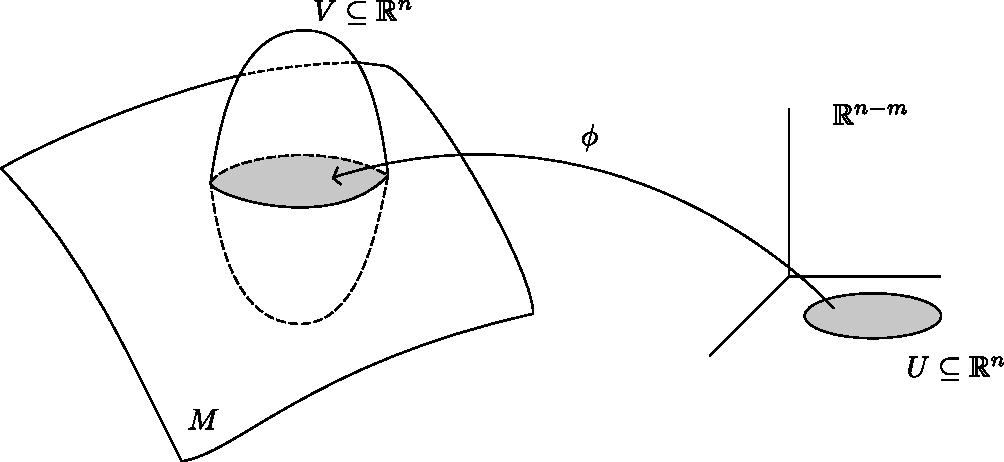
\includegraphics[width=0.75\textwidth]{Images/submanifold1.pdf}
     \caption{Submanifold - local parametrization}
\end{figure}
\end{definition}

\begin{definition}[Submanifold - Locally flat] \label{sub2}
  $M \subset \rfield^n$ is a submanifold of $\rfield^n$ if $\forall \, p  \,\in M$, there exists a neighbourhood $V \subset \rfield^n$ of $p$, a neighbourhood $W \subset \rfield^n$ of $0$, and a diffeomorphism $\Phi \colon V \rightarrow W$ such that:
  \[ \Phi(p)=0 \text{  and  } \Phi(V \cap M) = W \cap \left( \rfield^m \times \{0\}^{n-m} \right) \, .\]
  \begin{figure}[H]
  \label{Fig:submanifold2}
     \centering
     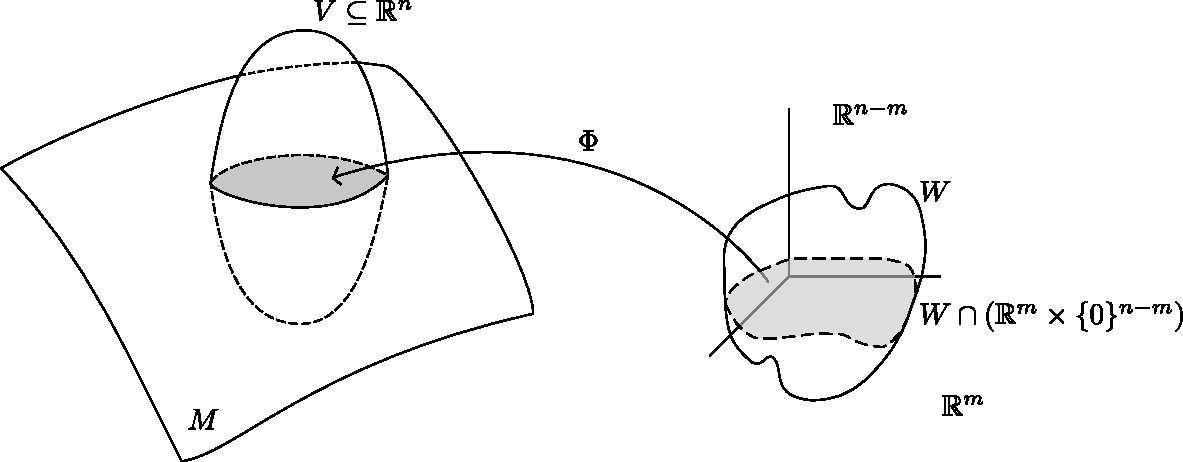
\includegraphics[width=0.8\textwidth]{Images/submanifold2.pdf}
     \caption{Submanifold - locally flat}
\end{figure}
\end{definition}

\begin{definition}[Submanifold - Locally  a zero set] \label{sub3}
$M \subset \rfield^n$ is a submanifold of $\rfield^n$ if
$\forall \, p \in M$ there exists an open neighbourhood $V \subset \rfield^n$ of $p$, and a smooth map $F \colon V \rightarrow \rfield^{n-m}$ such that:
\begin{itemize}
\item $V \cap M = \{x \in V \, | \, F(x) = 0\}$,
\item $F_* \colon V \rightarrow \rfield^{n-m}$ is surjective.
\end{itemize}

\begin{figure}[H]
  \label{Fig:submanifold3}
     \centering
     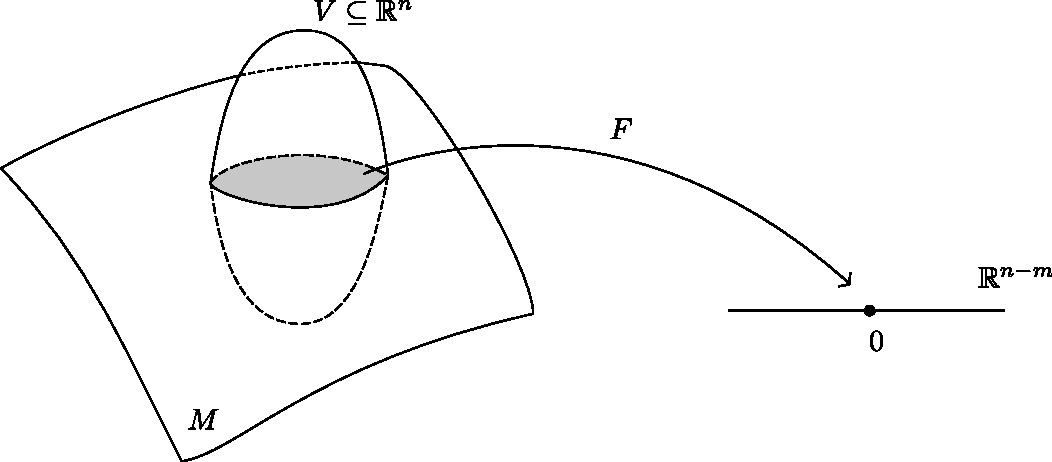
\includegraphics[width=0.8\textwidth]{Images/submanifold3.pdf}
     \caption{Submanifold - locally a zero set}
\end{figure}
\end{definition}

\begin{definition}[Submanifold - Locally a graph] \label{sub4}
  $M \subset \rfield^n$ is a submanifold of $\rfield^n$ if $\forall \, p \in M$ there exists a neighbourhood $V \subset \rfield^n$ of $p$, a permutation $\sigma \colon \{1, \ldots, n\} \rightarrow \{1, \ldots, n\}$ and an open set $U \subset \rfield^m, U$, together with a smooth map $g \colon U \rightarrow \rfield^{n-m}$ such that:
  \begin{align*}
  V \cap M = \{ &(x_{\sigma(1)}, \ldots, x_{\sigma(n)}) \, |\, (x_1, \ldots, x_m) \in U \\
   &\text{ and } (x_{m+1}, \ldots, x_n) = g(x_1, \ldots, x_m)\} \, .
\end{align*}
  The map g is called a \textit{graph}.
  \begin{figure}[H]
  \label{Fig:submanifold4}
     \centering
     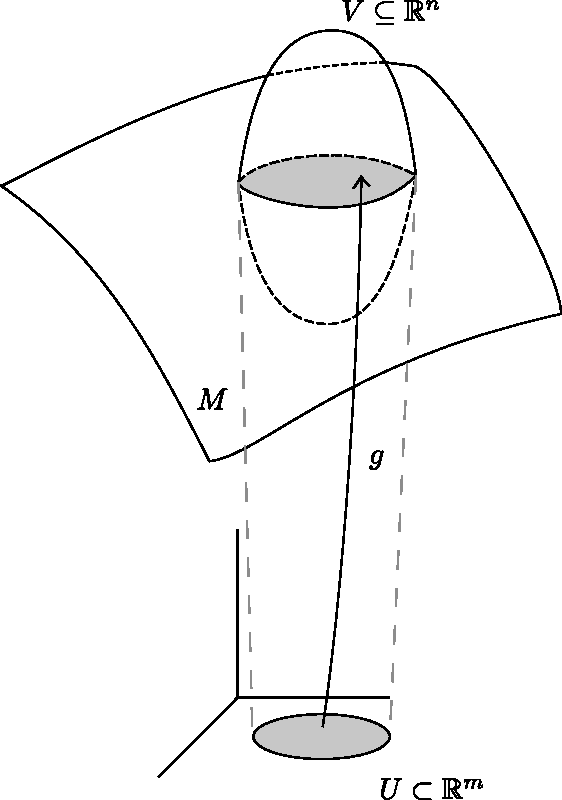
\includegraphics[width=0.4\textwidth]{Images/submanifold4.pdf}
     \caption{Submanifold - locally a graph}
\end{figure}
\end{definition}

\begin{remarkbox}\begin{remark}[4 definitions]
Let's analyze two of the four definitions of a submanifold of $\rfield^n$.
\begin{description}
\item[\ref{sub1})] The homeomorphism hypothesis is quite intuitive: we want our space to be locally similar to $\rfield^n$. In fact, the fact that $\phi$ is an isomorphism make the vector field given by the differential of $\phi$ well-defined. Indeed, the map $\phi$ can define a vector field on $M$ through its differential $d\phi=\phi_*$, if $\phi_*$ is a bijective map.
\begin{center}
\begin{minipage}{0.9\textwidth}
\vspace{1em}
     \centering
     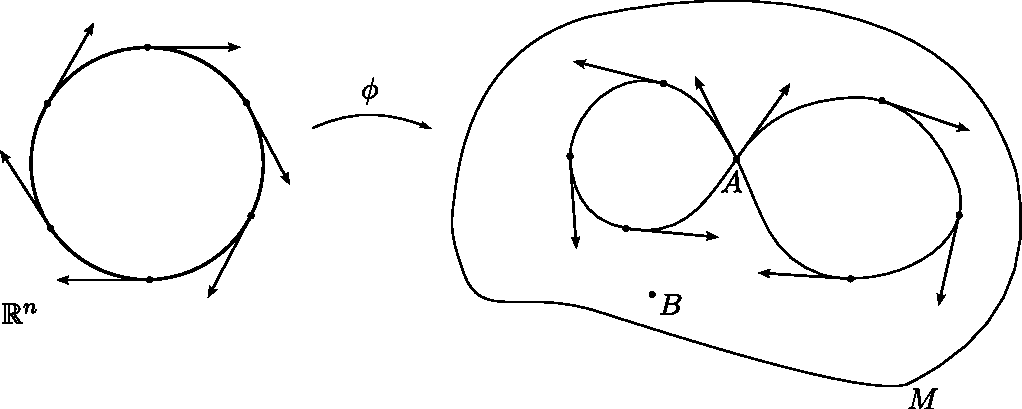
\includegraphics[width=0.9\textwidth]{Images/notinjnotsurj.pdf} \label{Fig:notinjnotsurj}
     \captionof{figure}{If $\phi$ is not injective, we have problems in $A$. If not surjective, we have problems in $B$ (see also page 182, \citetalias{Lee}).}
     \vspace{1em}
\end{minipage}
\end{center}
If $\phi$ is not injective, we would have some points on $M$ such that the tangent vector about these points is not unique: the physical meaning would be lost, and also the vector field given by the differential would not be well defined since it assigns more than one element to the initial vector.
If $\phi$ is not surjective, we would have some points on $M$ that have no tangent vector at all.
Moreover, we have the hypothesis of injectivity of $\phi_*$. It means that $\phi$ is a smooth embedding (see also the def. \ref{smoothembedd} that will be given in the next sections). Being a smooth embedding means that $U$ is being included in $V \cap M$. In fact, the Rank theorem (page 81 \citetalias{Lee}) says that a such a map behaves like an inclusion ($U$ is "injected" in $V \cap M$).
\item[\ref{sub3})] The hypothesis of surjectivity is required because of what we previously said about the Rank theorem. In particular, we require $F$ to be a smooth submersion (see also the def. \ref{smoothsubm} that will be given in the next sections). Using the Rank theorem, it means that the map $F$ behaves like a projection ($V \cap M$ is projected into the zero set). Notice that in this case we don't care about vector fields, so $F$ doesn't have to be bijective!
\end{description}
\end{remark}\end{remarkbox}

\begin{theorem} \label{allequiv}
  The four definitions above are equivalent.
\end{theorem}
\begin{proof} $ $
\begin{description}
\item[(b) $\Rightarrow$ (c):] $\Phi \colon W \rightarrow V$ is a diffeomorphism. Let $F(x) = \pi \circ \Phi^{-1}$, where $x \in M \cap V, \pi \colon \rfield^n \rightarrow \rfield^{n-m}$ ($\pi$ is the projection on the last $n-m$ coordinates). Then $F$ satisfies (c) by construction.
\item[(c) $\Rightarrow$ (d):] We have:
\begin{align*}
F \colon V \subset \rfield^m \times \rfield^{n-m} &\rightarrow \rfield^{n-m} \\
(a, b) & \mapsto F(a, b)
\end{align*}
Let's consider the Jacobian matrix:
\[
(F_*)_p = \left (
\begin{matrix}
\defonde{F^1}{x^1} & \ldots & \tikzmark{left}{\defonde{F^1}{x^{m+1}}} & \ldots & \defonde{F^1}{x^n} \\
\cdot & & & & \\
\cdot & & & & \\
\cdot & & & & \\
\defonde{F^{n-m}}{x^1} & \ldots & \defonde{F^{n-m}}{x^{m+1}} & \ldots & \tikzmark{right}{\defonde{F^{n-m}}{x^n}}
\end{matrix} \right)
\DrawBox[thick] \]
Let $A \in \rfield^{(n-m) \times (n-m)}$ be the submatrix denoted by the rectangle. $A$ is invertible because $F$ is surjective. Then, by Dini theorem (or implicit function theorem): $\exists\, U' \subset \rfield^m, U' $ open, $a \in U'$ and a map $g \colon U' \rightarrow \rfield^{n-m}$ such that $F(x_1, \ldots, x_m, x_{m+1}, \ldots, x_n)=0$ implies $(x_{m+1}, \ldots, x_n) = g(x_1, \ldots, x_m)$, where $(x_1, \ldots, x_m) \in U'$. Moreover, different orderings of columns of $A$ give rise to different permutations. Then, $g$ is the graph of definition (d).
\item[(d) $\Rightarrow$ (a):] From (d), we know that $g \colon \rfield^m \supset U \rightarrow \rfield^{n-m}$. Then:
\begin{align*}
\phi \colon U &\rightarrow \rfield^n = \rfield^m \times \rfield^{n-m} \\
x &\mapsto (x, g(x))
\end{align*}
is a local parametrization: it is a homeomorphism onto the image, and it is differentiable because $g$ is differentiable.
\item[(a) $\Rightarrow$ (b):] Let $\phi \colon \rfield^m \supset U \rightarrow \rfield^n$ be a local parametrization with $\phi_*\colon \rfield^m \rightarrow \rfield^n$ injective. Let
$$B \equiv \left( \left (\defonde{\phi^i}{x^j} \right)_{x=q} \right)_{i, j = 1, \ldots ,m}, \qquad q = \phi^{-1}(p), \, p \in M \cap V \, .$$
In general, it is not true that $\phi^1$ corresponds to the first component. But we can always reorder the coordinates so that it is true. $B$ is invertible. Let's define:
\begin{align*}
\Phi \colon U \times \rfield^{n-m} &\rightarrow \rfield^n= \rfield^m \times \rfield^{n-m} \\
(x, y) &\mapsto \phi(x) + (0, y) =  \\ &= ( \phi_1(x_1, \ldots, x_m), \ldots, \phi_m(x_1, \ldots, x_m), \\
& \phi_{m+1}(x_1, \ldots, x_m) + y_1, \ldots, \phi_n(x_1, \ldots, x_m) + y_{n-m} ) \, .
\end{align*}
Then:
\[ \Phi_*(q, 0) = \left (
\begin{array}{c|c}
B & 0 \\
\hline
\text{anything} & \text{Id}
\end{array} \right) \]
is invertible. Thus, by the implicit function theorem, there exists a neighbourhood $W \subset (U \times \rfield^{n-m})$ of $(q, 0)$ and $V' \subset \rfield^n$ of $p$ such that $\Phi \colon W \rightarrow V'$ is a diffeomorphism. Furthermore:
\[ \Phi\left ( W \cap (\rfield^m \times \{0\}^{n-m}) \right) = \phi\left( W \cap (\rfield^m \times \{0\}^{n-m}) \right) \subset M \cap V \]
because $\Phi$ acts like $\phi$ for $y=0$. The local inverse of $\Phi$ satisfies the definition (b).
\end{description}
\end{proof}

\begin{corollary} \label{corsubmanifold}
  Let:
  $$\phi \colon \rfield^m \supset U \rightarrow V \cap M$$
  $$\phi' \colon \rfield^m \supset U' \rightarrow V' \cap M$$
  be local parametrizations. Then:
  $$\phi^{-1} \circ \phi' \colon (\phi')^{-1} (\phi(U) \cap \phi'(U')) \rightarrow \phi^{-1}(\phi(U) \cap \phi'(U'))$$
  is a diffeomorphism. %write that they are open sets? intersection color...check
\end{corollary}
\begin{center}
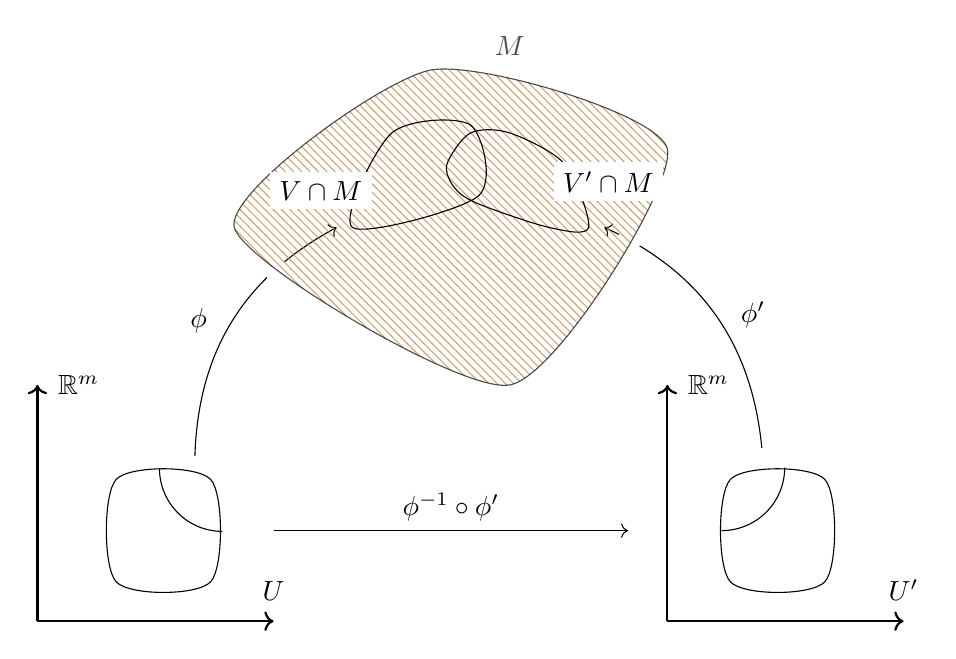
\begin{tikzpicture}

    % Functions i
    \path[->] (-1, -2.9) edge [bend left] node[left, xshift=-2mm] {$\phi$} (0.8, 0);
    \draw[white,fill=white] (0.06,-0.57) circle (.15cm);


    % Functions j
    \path[->] (6.2, -2.8) edge [bend right] node[right, xshift=2mm] {$\phi'$} (4.2, 0);
    \draw[white, fill=white] (4.54,-0.12) circle (.15cm);

    % Manifold
    \draw[smooth cycle, tension=0.4, fill=white, pattern color=brown, pattern=north west lines, opacity=0.7] plot coordinates{(2,2) (-0.5,0) (3,-2) (5,1)} node at (3,2.3) {$M$};

    % Help lines
    %\draw[help lines] (-3,-6) grid (8,6);

    % Subsets
    \draw[smooth cycle]
        plot coordinates {(1,0) (1.5, 1.2) (2.5,1.3) (2.6, 0.4)}
        node [label={[label distance=-0.3cm, xshift=-2cm, fill=white]:$V \cap M$}] {};
    \draw[smooth cycle]
        plot coordinates {(4, 0) (3.7, 0.8) (3.0, 1.2) (2.5, 1.2) (2.2, 0.8) (2.3, 0.5) (2.6, 0.3) (3.5, 0.0)}
        node [label={[label distance=-0.8cm, xshift=.75cm, yshift=1cm, fill=white]:$V' \cap M$}] {};

    % First Axis
    \draw[thick, ->] (-3,-5) -- (0, -5) node [label=above:$U$] {};
    \draw[thick, ->] (-3,-5) -- (-3, -2) node [label=right:$\mathbb{R}^m$] {};

    % Arrow from i to j
    \draw[->] (0, -3.85) -- node[midway, above]{$\phi^{-1} \circ \phi'$} (4.5, -3.85);

    % Second Axis
    \draw[thick, ->] (5, -5) -- (8, -5) node [label=above:$U'$] {};
    \draw[thick, ->] (5, -5) -- (5, -2) node [label=right:$\mathbb{R}^m$] {};

    % Sets in R^m
    \draw[white, ] (-0.67, -3.06) -- +(180:0.8) arc (180:270:0.8);
    \fill[even odd rule, white] [smooth cycle] plot coordinates{(-2, -4.5) (-2, -3.2) (-0.8, -3.2) (-0.8, -4.5)} (-0.67, -3.06) -- +(180:0.8) arc (180:270:0.8);
    \draw[smooth cycle] plot coordinates{(-2, -4.5) (-2, -3.2) (-0.8, -3.2) (-0.8, -4.5)};
    \draw (-1.45, -3.06) arc (180:270:0.8);

    \draw[white] (5.7, -3.06) -- +(-90:0.8) arc (-90:0:0.8);
    \fill[even odd rule, white] [smooth cycle] plot coordinates{(7, -4.5) (7, -3.2) (5.8, -3.2) (5.8, -4.5)} (5.7, -3.06) -- +(-90:0.8) arc (-90:0:0.8);
    \draw[smooth cycle] plot coordinates{(7, -4.5) (7, -3.2) (5.8, -3.2) (5.8, -4.5)};
    \draw (5.69, -3.85) arc (-90:0:0.8);

\end{tikzpicture}
\end{center}
\begin{proof}
$\phi^{-1} \circ \phi'$ is a homeomorphism because $\phi$ and $\phi'$ are homeomorphisms. We want to show that they are smooth. Let:
\begin{align*}
&q' \in (\phi')^{-1}(\phi(U) \cap \phi'(U')) \subset U' \\
&q \in \phi^{-1} \circ \phi' (q') \in U \, .
\end{align*}
By the proof of (a) $\Rightarrow$ (b) of the theorem \ref{allequiv}, we know that there exists a diffeomorphism $\Phi \colon \rfield^n \supset W \rightarrow V'' \subset \rfield^n$, with $(q, 0) \in W$, such that:
\[ \restrict{\Phi}{W \cap \rfield^m} = \restrict{\phi}{W \cap \rfield^m} \, . \]
Thus:
\[\restrict{\phi^{-1} \circ \phi'}{(\phi')^{-1} \circ \phi(W \cap \rfield^m)} = \restrict{\Phi^{-1} \circ \phi'}{(\phi')^{-1} \circ \phi(W \cap \rfield^m)} \]
where the right-hand side is smooth. We can prove the same result the other way round.
\end{proof}

\begin{tcolorbox}\begin{example}[Submanifolds of $\rfield^n$]
  Let's consider some examples.
  \begin{enumerate}
    \item An open subset of dimension $n$ in $\rfield^n$ is a submanifold (by definition (a), we just take $\phi = \id$). For instance $B^n\subset \rfield^n$ is a submanifold of $\rfield^n$.
    \item $S^{n-1} = \partial B^n$ is a submanifold of $\rfield^n$. Indeed, by definition (c), it is the zero set of the function:
    $$F(\underline{x}) = (x^1)^2 + (x^2)^2 + \ldots + (x^n)^2 - 1 = \underline{x}^2 -1, \, \underline{x} \in \rfield^n$$
    and $F_*$ is surjective: $F_*(\underline{x}) = 2 \underline{x}$.
    \item $O(n) = \{A \, | \, AA^t = E\} \subset Mat(n \times n, \rfield) \cong \rfield^{n^2}$, with $E$ identity matrix. $O(n)$ is a submanifold of dimension $\frac{n(n-1)}{2}$. Indeed, using definition (c), it is the zero set of the function:
    \begin{align*}
      F \colon Mat(n \times n, \rfield) &\rightarrow Symm(n, \rfield) \\
      A &\mapsto AA^t - E \, .
    \end{align*}
    What is more, $F_*$ is surjective. In order to prove that, we prove that "$\restrict{F_*}{A}(X)=0, \forall\, A \Rightarrow X = 0$" (then we know that for a linear map $L$ on a vector space $V$, $\dim(V) = \dim Ker(L) + \dim Ran(L)$, so the dimension of the range of $\restrict{F_*}{A}$ must be $\dim Mat(n\times n, \rfield)$, so the map is surjective).
    In fact:
    \begin{align*}
    \restrict{F_*}{A} &= \restrict{\frac{d}{dt}}{t=0}F(A + tX) = \restrict{\frac{d}{dt}}{t=0} \left[ AA^t + tAX^t + tXA^t + t^2XX^t \right] = \\
    & = AX^t + XA^t \, .
  \end{align*}
    And the solution of:
    $AX^t + XA^t = S \in Symm(n, \rfield)$
    is $X = \frac{SA}{2}$ because $\frac{AA^t}{2}S + S\frac{AA^t}{2} = S$.
    Then:
    $$AX^t + XA^t = 0 \Longrightarrow X=0 \, .$$
  \end{enumerate}
\end{example}\end{tcolorbox}

Now, we want to use diffeomorphisms like those in the corollary \ref{corsubmanifold} in order to introduce the concept of manifold.

\begin{definition}[Atlas] \label{atlasdef}
  An (n-dimensional, smooth) atlas $\mathcal{A}$ on a set $M$ is a collection of maps (called charts)
  \begin{align}
    \phi_{\alpha} \colon \rfield^n &\overset{\sim}{\rightarrow} M \\
    U_{\alpha} &\mapsto W_{\alpha} \nonumber
  \end{align}
  such that:
  \begin{itemize}
    \item $\bigcup\limits_{\alpha \in I} W_{\alpha} = M$,
    \item $\forall\, \alpha, \beta \in I$ with $W_{\alpha} \cap W_{\beta} \not = \emptyset$,
    $$\phi^{-1}_{\beta} \circ \phi_{\alpha} \colon \phi^{-1}_{\alpha}(W_{\alpha} \cap W_{\beta}) \rightarrow \phi_{\beta}^{-1}(W_{\alpha} \cap W_{\beta})$$
    is a diffeomorphism.
  \end{itemize}
  where $\alpha \in I, I$ index set, and the $\sim$ above the arrow means that $\phi_{\alpha}$ is bijective.
\end{definition}

\begin{definition} [Equivalence relation on atlases]
  Two atlases $\mathcal{A}$ and $\mathcal{A'}$ are equivalent $\Leftrightarrow$ $\mathcal{A} \cup \mathcal{A'}$ is an atlas ($\Leftrightarrow \phi_{\beta}^{-1} \circ \phi_{\alpha}'$ is a diffeomorphism, $\forall\, \phi_{\alpha}' \in \mathcal{A}', \phi_{\beta} \in \mathcal{A})$.
\end{definition}

\begin{definition}[\textbf{Preliminary} definition of manifold] \label{manifoldprel}
  A manifold is a set $M$ with an equivalence class of atlases.
\end{definition}

\begin{remarkbox}\begin{remark}
  The definition \ref{manifoldprel} above is "\textit{preliminary}" because we have not specified anything about the topology yet (we are still working on Euclidean topology). Moreover, in every equivalence class there exists a unique maximal atlas (i.e. such that, if combined with an other atlas, it can't get any bigger). We also notice that if the charts are smooth enough, we can pullback "everything" (e.g. all our vector fields, differential forms, etc. defined for subset of $\rfield^n$). However, in that case, everything is defined \textit{locally}. In order to patch them all together, we need some other result (like the partition of unity, coming soon).
\end{remark}\end{remarkbox}

\begin{tcolorbox}\begin{example}[Projective space]
  Let $\mathbb{K} \in \{\rfield, \mathbb{C}\}$ ($\mathbb{K}$ is some field).
  $$\mathbb{K}P^n \equiv \faktor{(\mathbb{K}^{n+1} \setminus \{0\})}{\sim}$$
  where
  \begin{align*}&(x_0, \ldots, x_n) \sim (x_0', \ldots, x_n') \Longleftrightarrow \\
     \exists \, \lambda \in \mathbb{K}\setminus \{0\} &\text{ such that } (\lambda x_0, \ldots, \lambda x_n) = (x_0', \ldots, x_n') \, .
  \end{align*}
  For instance, $\mathbb{C}P^1 = S^2$ (every point on a line passing through the origin is identified with the point on such line at distance 1 from the origin). We use the notation $[x_0, \ldots, x_n]$ for one equivalence class.
  Let's consider the atlas $\mathcal{A} = \{\phi_i \colon \mathbb{K}^n \rightarrow \mathbb{K} P^n \}$. Where
  \begin{align*}
    \phi_i \colon \mathbb{K}^n &\rightarrow \mathbb{K}P^n \\
    (x_0, \ldots, x_{i-1}, x_{i+1}, \ldots, x_n) &\mapsto [x_0, \ldots, x_{i-1}, 1, x_{i+1}, \ldots, x_n]
  \end{align*}
  And $\phi_i(\mathbb{K}^n) = \left\{[x_0, \ldots, x_n] \in \mathbb{K}P^n \, | \, \text{ i-th entry is } \not = 0 \right \}$.
  We notice that $\mathcal{A}$ is an atlas because $\phi_i$ satisfies the properties of the definition \ref{atlasdef}:
  \begin{itemize}
    \item $\phi$ is a bijection and its inverse is
    \begin{align*}
      \phi_i^{-1} \colon \phi_i(\mathbb{K}^n) & \rightarrow \mathbb{K^n} \\
      [x_0, \ldots, x_{i-1}, \underbrace{x_i}_{\not = 0}, \ldots, x_n] &\mapsto \left( \frac{x_0}{x_i}, \frac{x_1}{x_i}, \ldots, \frac{x_{i-1}}{x_i}, \frac{x_{i+1}}{x_i}, \ldots, \frac{x_n}{x_i} \right)
    \end{align*}
    \item $\phi$ is also a diffeomorphism, because $\phi_j^{-1} \circ \phi_i$, defined as
    \begin{align*}
      \phi_j^{-1} \circ \phi_i \colon \phi_i^{-1} \left(\phi_i(\mathbb{K}^n) \cap \phi_j(\mathbb{K}^n) \right) &\rightarrow \phi_j^{-1} \left(\phi_i(\mathbb{K}^n) \cap \phi_j(\mathbb{K}^n) \right) \\
      (x_1, \ldots, x_n) &\mapsto \Bigl( \frac{x_1}{x_j}, \ldots, \underbrace{\frac{1}{x_j}}_{i-th}, \ldots, \frac{x_n}{x_j} \Bigr)
    \end{align*}
    is a diffeomorphism (where $x_i \not = 0, x_j \not = 0$) because it is a differentiable map and the inverse is again differentiable.
  \end{itemize}
\end{example}\end{tcolorbox}

\begin{remarkbox}\begin{remark}[Extension of analysis to manifolds]
  The existence of an atlas allows us to define concepts from analysis to manifolds. For instance, we can define continuous and smooth functions on manifolds using the concepts of continuity and smoothness that we use in $\rfield^n$.
\end{remark}\end{remarkbox}

\begin{definition}[Continuous/smooth function on a manifold]
  Let $M$ be a manifold, a function $f \colon M \rightarrow \rfield$ is a continuous (respectively, smooth) function if and only if $f \circ \phi_{\alpha} \colon U_{\alpha} \rightarrow \rfield$ is continuous (smooth) function $\forall \, \alpha$. Such a function is well-defined, since the definition is independent on the local parametrization chosen, thanks to the definition of atlas.
\end{definition}

\begin{remarkbox}\begin{remark}[cut-off functions]
  We can construct functions on a manifold in the following way: we consider a function defined on an open set in $M$ which is homeomorphic to an open set in $\rfield^n$. Then we extend it to zero outside such open set, but in order to have a differentiable function we smoothly bring it to zero using the so-called cut-off functions.
  For instance, a smooth function from $\rfield$ to $[0, 1] \subset \rfield$ such that:
  \begin{equation*}
    h(x) = \begin{cases*}
     1, & $x \le 1$ \\
     \text{anything}, &  $1 \le x \le 2$ \\
     0, & $x \ge 2$
  \end{cases*}
  \end{equation*}
  is a cut-off function.
  For example, given
  \begin{equation*}
    a(x) = \begin{cases*}
     0, & $x \le 0$ \\
     e^{-1/x}, & $x \ge 0$
  \end{cases*}
  \end{equation*}
  we can consider
  \begin{equation*}
    g(x) = 1 - \frac{a(x)}{a(x) + a(1-x)} \, .
  \end{equation*}
  \begin{figure}[H]
  \centering
  \begin{subfigure}{.5\textwidth}
    \centering
    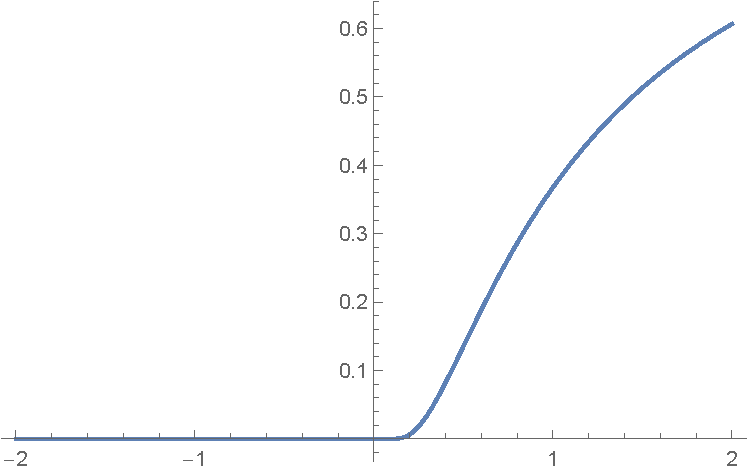
\includegraphics[width=.9\linewidth]{Images/cutoff_1.pdf}
    \caption{$a(x)$}
  \end{subfigure}%
  \begin{subfigure}{.5\textwidth}
    \centering
    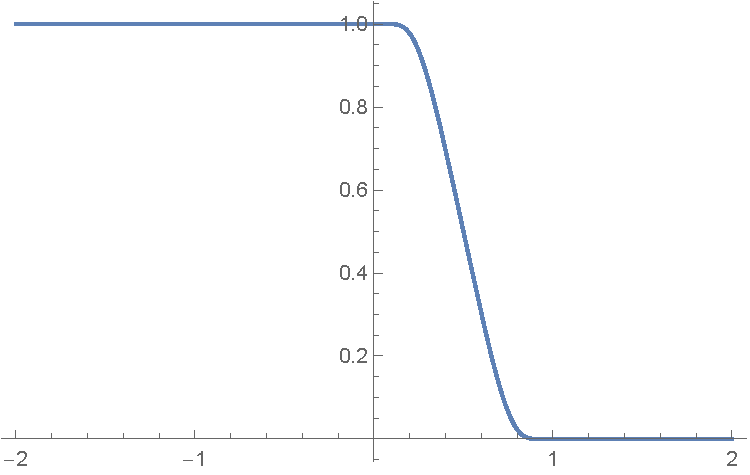
\includegraphics[width=.9\linewidth]{Images/cutoff_2}
    \caption{$g(x)$}
  \end{subfigure}
  \end{figure}
  Then we use the function 
  \begin{equation*}
    h_{\epsilon}(x) \equiv h \left (\frac{x}{\epsilon} \right) =
    \begin{cases*}
      1, & $x \le \epsilon$ \\
      0, & $x \ge 2 \epsilon$
    \end{cases*}
  \end{equation*}
  Now, for $p \in M$, let
  $$\phi \colon \rfield^n \supset U \rightarrow V \subset M$$
  such that $\phi(0) = p$ (where $0 \in U$) and $\epsilon > 0$ such that $B_{3 \epsilon} \supset U $. %subset?check

  \begin{figure}[H]
          \centering
  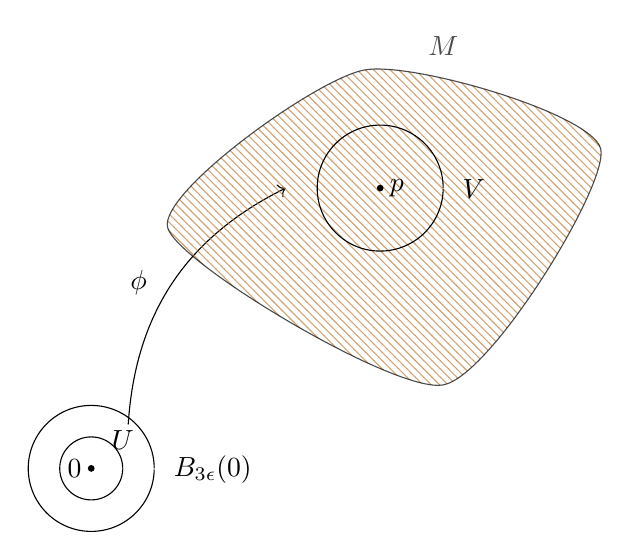
\begin{tikzpicture}
      % Functions i
      \path[->] (-1, -2.5) edge [bend left] node[left, xshift=-2mm] {$\phi$} (1, 0.5);
      \draw[white,fill=white] (0.06,-0.57) circle (.15cm);

      % Manifold
      \draw[smooth cycle, tension=0.4, fill=white, pattern color=brown, pattern=north west lines, opacity=0.7] plot coordinates{(2,2) (-0.5,0) (3,-2) (5,1)} node at (3,2.3) {$M$};

      % Help lines
      %\draw[help lines] (-3,-6) grid (8,6);

      % Subsets
      %\draw[smooth cycle]
          \draw (3, 0.5) arc (0:359:0.8) node [label=right: $V$]{};
          \filldraw[black] (2.2, 0.5) circle (1pt) node[anchor=west] {$p$};
          %\draw[white, pattern color=blue, pattern=crosshatch dots] (5.7, -3.06) -- +(-90:0.8) arc (-90:0:0.8);
          %plot coordinates {(1,0) (1.5, 1.2) (2.5,1.3) (2.6, 0.4)}
          %node [label={[label distance=-0.3cm, xshift=-2cm, fill=white]:$V \cap M$}] {};

      % Sets in R^m
      \draw (-0.67, -3.06)  arc (0:359:0.8) node [label=right: $B_{3 \epsilon}(0)$] {};
      \draw (-1.07, -3.06)  arc (0:359:0.4) node [label=above: $ U$] {};
      \filldraw[black] (-1.47, -3.06) circle (1pt) node[anchor=east] {$0$};

  \end{tikzpicture}
\end{figure}
  Then $g(x) = h_{\epsilon}(|x|)$ defines a smooth function $g \colon \rfield^n \rightarrow \rfield$ with supp$(g) = \overline{\{ x \, | \, g(x) \not =  0\}} \subset U$. Moreover, $g \circ \phi^{-1} \colon V \rightarrow \rfield$ extends (by zero) to a function $f \in \mathbb{F}(M)$ with supp$f \subset V$ and $f \equiv 1$ in a neighbourhood of $p$. In particular, this shows that $\mathbb{F}(M)$ is infinite-dimensional.


\end{remark}\end{remarkbox}

\begin{definition}[Vector fields on manifolds]
  Vector fields are defined as before (we just replace $\mathbb{F}(\rfield^n)$ with $\mathbb{F}(M)$). They are maps
  $$\restrict{\Der}{p} \mathbb{F}(M) = T_p M \ni v_p \colon \mathbb{F}(M) \rightarrow \rfield$$
  which are $\rfield$-linear and satisfying Leibnitz rule.
  The set of all vector fields is:
  $$\mathfrak{X}(M) = \Der \mathbb{F}(M) = TM \ni v \colon \mathbb{F}(M) \rightarrow \mathbb{F}(M)$$

\end{definition}

\begin{remarkbox}\begin{remark}[Representation of $v$ in $U_{\alpha}$, local coordinates]
  Everything is done in $\rfield^n$. Indeed, if $(\phi_{\alpha}, U_{\alpha})$ is a chart, with $U_{\alpha} \subset \rfield^n$, $\phi_{\alpha}$ is called a local coordinate map. Then, the representation of a vector field $v$ in $U_{\alpha}$ is:
  $$v_{(\alpha)} = v_{(\alpha)}^i \partial_{x_i}$$
  where
  $$v_{(\alpha)}^i(x) = v^i \circ \phi_{\alpha}(x) \, .$$
  We point out that given a chart $(\phi_{\alpha}, U_{\alpha})$ and a point $x$ in the manifold, the local coordinates of $x$ with respect to the chart are the coordinates of $\phi_{\alpha}(x)$ as a vector in $U_{\alpha} \subset \rfield^n$. (Here, we are denoting the chart by using the subset of $	\rfield^n$, and not the subset of the manifold. Since $\phi$ is a diffeomorphism we can do that.)
\end{remark}\end{remarkbox}

Notice that cut-off functions allow us to extend any smooth function defined on $V_{\alpha} \subset M$ (for some $\alpha \in I$) to all of $M$ through extension by zero outside $V_{\alpha}$.
Suppose we are given a function on $M$. How do we decide if it is continuous (or smooth)?
\begin{proposition}[Partition of unity]
Let $M$ be a compact manifold and let $\{V_{\alpha}\}$ be a covering of $M$. Then there exists a family of differentiable functions $\varphi_1, \ldots, \varphi_m$ such that:
\begin{itemize}
  \item $\sum\limits_{i=1}^m \varphi_i \equiv 1$,
  \item $0 \le \varphi_i \le 1$ and supp$(\varphi_i) \subset V_{\alpha}$ for some $\alpha \in I$.
\end{itemize}
\end{proposition}

\begin{definition}[Partition of unity]
  The family $\{\varphi_i\}$ defined above is said to be a partition of unity subordinate to the covering $\{V_{\alpha}\}$.
\end{definition}

Now, if $f \colon M \rightarrow \rfield$, we can consider $f_i = \varphi_i f \colon v_{\alpha} \rightarrow \rfield$ for some $\alpha \in I$.

\begin{definition}[Differential forms on M] A differential form on $M$ is a map
  \begin{align}
    \Omega^k(M) \ni \omega \colon \mathfrak{X}(M) \times \cdots \times \mathfrak{X}(M) &\rightarrow \mathbb{F}(M) \\
    (v_1, \ldots, v_k) &\mapsto \omega(v_1, \ldots, v_k) \nonumber
  \end{align}
  which is linear, skew-symmetric (i.e. alternating) as already defined.
\end{definition}

\begin{remarkbox}\begin{remark}[Representation of $\omega$ in $U_{\alpha}$]
  We represent $\omega$ in $U_{\alpha}$ as:
  $$\omega_{(\alpha)} = \sum\limits_{i_1 < \cdots < i_k} (a_{i_1 \cdots i_k})_{(\alpha)} dx^{i_1} \wedge \ldots \wedge dx^{i_k}$$
  where $\{x^i\}$ are the coordinates on $U_{\alpha}$.
  Moreover:
  $$\omega_{(\alpha)} ((v_1)_{\alpha}, \ldots, (v_k)_{\alpha}) = \pm \sum\limits_{i_1 < \cdots < i_k} (a_{i_1\cdots i_k})_{\alpha} (v^{i_1})_{\alpha} \cdots (v^{i_k})_{\alpha}$$
  where the $\pm$ sign depends on the orientation used.
\end{remark}\end{remarkbox}

\begin{definition}[Curve on a manifold]
  A curve $\gamma \colon (a, b) \rightarrow M$ is continuous (respectively, differentiable) if $\phi_{\alpha}^{-1} \circ \gamma \colon (a, b) \rightarrow U_{\alpha}$ is continuous (differentiable).
\end{definition}
\section[Integration on Compact Manifolds]{\crule[orange!50!white]{0.3cm}{0.4cm}  Integration on Compact Manifolds}

\begin{definition} [Orientable manifold]
  $M$ is orientable if there exists an atlas $\mathcal{A} = \{\phi_{\alpha}, U_{\alpha}\}$ such that for each pair $\alpha, \beta$ with $\phi_{\alpha}(U_{\alpha}) \cap \phi_{\beta}(U_{\beta}) \not = \emptyset$, the differential
  $$
    (\phi_{\beta}^{-1} \circ \phi_{\alpha})_* \colon  U_{\alpha} \rightarrow U_{\beta}
  $$
  has positive determinant. Example of a non-orientable manifold: Möbius strip.
\end{definition}

\begin{remarkbox}\begin{remark}[How to integrate]
Let $\omega \in \Omega^n(M), M \text{ compact manifold }, \dim M=n$. Pick a partition of unity subordinate to a covering $\{V_{\alpha} \}$ (i.e. pick some maps $\varphi_i, i=1, \ldots, n, 0 \le \varphi_i \le 1, \sum_{i=1}^m \varphi_i \equiv 1, \text{ supp}(\varphi_i) \subset V_{\alpha(i)}$ for some $\alpha = \alpha(i)$). Then:
\begin{align}
  \int\limits_M \omega &= \int\limits_M \sum_{i=1}^m \varphi_i \omega = \sum_i \int\limits_M (\varphi_i \omega) = \sum_i \int\limits_{V_{\alpha(i)}} (\varphi_i \omega) = \nonumber \\
  & = \sum_i \int\limits_{U_{\alpha(i)}} \phi^*_{\alpha(i)} (\varphi_i \omega)
\end{align}
where $V_{\alpha} = \phi_{\alpha}(U_{\alpha})$.
Notice that \textbf{the integral is well-defined if $M$ is orientable}: if it's not, when we make a change of coordinates to swap to another chart we get a different sign. Indeed, the formula of the change of coordinate contains the determinant of the Jacobian, and we would find a chart that gives us a different final sign.
\end{remark}\end{remarkbox}

\begin{lemma}
  $\int\limits_{M} \omega$ is independent of the choice of $(V_{\alpha}, \varphi_i)$.
\end{lemma}
\begin{proof}
Let $\{ W_{\alpha} \}$ be another covering of $M$ and $\{\psi_j\}_{j=1, \ldots, m'}$ a partition of unity
 subordinate to $\{W_{\alpha}\}$,
 then $\{W_{\alpha} \cap V_{\beta}\}_{\alpha, \beta}$ is also
  a covering of $M$ and
  \[ \left(\varphi_i \psi_j \right)_{\substack{i=1, \ldots, m \\ j=1, \ldots, m'}}\]
  is a partition of unity subordinate to $\{W_{\alpha} \cap V_{\beta}\}$. Thus:
\[ \sum\limits_{i=1}^m \int_M \varphi_i \omega = \sum\limits_{i=1}^m \sum_{j=1}^{m'} \int_M \varphi_i \psi_j \omega = \sum\limits_{j=1}^{m'} \int_M \psi_j \left( \sum\limits_{i=1}^{m} \varphi_i \omega \right) = \sum\limits_{j=1}^{m'} \int_M \psi_j \omega \]
where we could swap the sums since they are finite (they are finite because $M$ is compact by assumption).
\end{proof}

\begin{remarkbox}\begin{remark}
  What happens with boundaries? If $p \in \partial M$, there is no neighbourhood of $p$ homeomorphic to an open set $U \subset \rfield^n$.
  Let's define the following set:
  $$H^n = \{ (x^1, \ldots, x^n) \in \rfield^n \, | \, x^1 \ge 0 \} \, .$$
  \textbf{Note} that on \citetalias{Lee}, $H^n$ is defined as
  $$H^n = \{ (x^1, \ldots, x^n) \in \rfield^n \, | \, x^n \ge 0 \}$$
  (everything is the same, but with $x^1$ replaced by $x^n$).
\end{remark}\end{remarkbox}

\begin{definition}[subset topology in $H^n$]
  An open set in $H^n$ is the intersection between $H^n$ and an open set in $\rfield^n$.
\end{definition}

\begin{definition}[Functions on $H^n$]
  A function $f \colon V \rightarrow \rfield, V$ open, $V \subset H^n$ is differentiable if $\exists$ an open set $U, \rfield^n \supset U \supset V$ and a differentiable function
  $\bar f \colon U \rightarrow \rfield$ such that $\restrict{\bar f}{V} = \restrict{f}{V}$.
  Furthermore, $(f_*)_p = (\bar f_*)_p, p \in V$.
\end{definition}

\begin{definition}[\textbf{Preliminary} definition of diff. manifold with boundary]
  An $n$-dimensional differentiable manifold with a regular boundary is a set $M$ with an equivalence class of atlases, as usual, but with the difference that $\rfield^n$ in the definition \ref{atlasdef} is replaced by $H^n$ everywhere. The boundary is "regular" if it is described by a regular curve (no intersection, etc...).
\end{definition}

When is a point on the boundary of a manifold?
\begin{definition} [Point on the boundary] \label{pointbdr}
  A point $p \in M$ is on the boundary of $M$ if for some parametrisation $\phi \colon U \subset H^n \rightarrow M$ around $p$, we have $\phi(0, x^2, \ldots, x^n) = p$ for some $x^2, \ldots, x^n$.
  \begin{figure}[H]
     \centering
     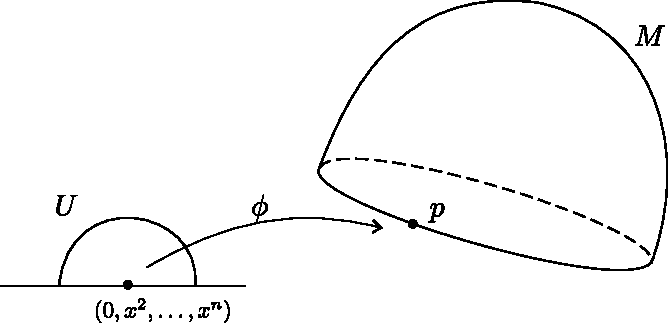
\includegraphics[width=.6\linewidth]{images/boundary.pdf}
     \caption{Point on the boundary of a manifold} \label{Fig:boundarypic}
\end{figure}
\end{definition}

\begin{lemma}
  The definition \ref{pointbdr} does not depend on the choice of parametrisation.
\end{lemma}
\begin{proof}
The proof is by contradiction.
Let $\phi_1 \colon U_1 \rightarrow M, U_1 \subset H^n$ such that $\phi_1(0, x^2, \ldots, x^n)=p$ for some $x^2, \ldots, x^n$. Assume there exists $\phi_2 \colon U_2 \rightarrow M$ parametrization around $p$ such that $\phi_2^{-1}(p) = q = (x^1, \ldots x^n)$ with $x^1 \not = 0$. Let $\Omega = \phi_1(U_1) \cap \phi_2(U_2)$. Then, the map:
\[\left ( \phi_1^{-1} \circ \phi_2 \right) \colon \phi_2^{-1}(\Omega) \rightarrow \phi_1^{-1}(\Omega)\]
is a diffeomorphism (by definition of manifold). Since $x^1 \not = 0$, there exists a neighbourhood $U$ of $q$ such that $U \subset \phi_2^{-1}(\Omega)$ and such that $U$ does not intersect with:
\[\left \{ (x^1, \ldots , x^n ) \in H^n \, | \, x^1= 0 \right \} \, . \]
The restriction of $\phi_1^{-1} \circ \phi_2$ to $U$ gives a differentiable map $U \rightarrow H^n$ such that $\det(\phi_1^{-1} \circ \phi_2)_* \not = 0$ (invertible map). Thus, $H^n$ is diffeomorphic to a set that doesn't contain $\{ (x^1, \ldots, x^n) | x^1 = 0 \}$, contradiction.
\end{proof}

\begin{proposition}
$ $
  \begin{itemize}
    \item The boundary $\partial M$ of a $n$-dimensional differentiable manifold with boundary is a $(n-1)$-dimensional differentiable manifold, %with boundary?check
    \item The orientation on $M$ induces an orientation on $\partial M$.
  \end{itemize}
\end{proposition}

\begin{theorem}[Stokes theorem on manifolds]
  $M$ orientable, then:
  \begin{equation}
    \int\limits_M d \omega = \int\limits_{\partial M} i^* \omega \, .
  \end{equation}
\end{theorem}
\begin{proof}[Idea of the proof]
First, we prove the theorem for a rectangle and then, for a generic set, we fill the set itself with rectangles.
\end{proof}

\section[Abstract Manifolds]{\crule[red!50!white]{0.3cm}{0.4cm}  Abstract Manifolds}
\begin{remarkbox}\begin{remark}[Non-Example of a manifold]
The set $$M= (-\infty, 0) \cup (0, \infty) \cup \{a, b\}$$ (endowed with a particular topology that we will see later) is not a manifold. Here, $a, b$ can be seen as points of $\rfield^2$: just imagine $M$ as a subset of $\rfield^2$, consisting of a real line without the origin plus any two points in $\rfield^2$. Even if we have not defined a topology on $M$, we can feel that it doesn't look right: there are two maps $\varphi_a, \varphi_b$ identifying the subsets $U_a = M \setminus \{b\}$ and $U_b = M \setminus \{a\}$ with $\rfield$. Indeed, in the first case the 0 element is given by the point $a$, whereas in the second case the 0 is given by $b$. The transition function
$$\varphi_b \circ \varphi_a^{-1} \colon \varphi_a(U_a \cap U_b) = \rfield \setminus \{0\} \rightarrow \varphi_b(U_b \cap U_a) = \rfield \setminus \{0\}$$
is the identity, and is smooth. \textbf{But}  a smooth function on $M$ must have the same value when evaluated at $a$ and $b$, and this does not look right (why?).
\end{remark}\end{remarkbox}



\begin{definition}[Manifold]
A manifold $M$ of dimension $n$ is a topological space which is Hausdorff, second countable and admits an (equivalence class of) atlas(es) $\varphi_i \colon U_i \rightarrow V_i$, where the
$\varphi_i$ are homeomorphisms, $U_i \subset M$ is open and $V_i \subset \rfield^n$ is also open, so that the transition functions
$$\varphi_i \circ \varphi_j^{-1} \colon \varphi_j(U_i \cap U_j) \rightarrow \varphi_i (U_i \cap U_j)$$ are smooth (i.e. $C^{\infty}$). Sometimes we consider $\varphi$ going from $\rfield^n$ to $M$ instead that the other way around, without any loss of generality. Notice that we are considering equivalence classes of atlases. We recall that the equivalence relation is the following one: two atlases are equivalent if their union is still a smooth atlas.
\end{definition}

\begin{remarkbox} \begin{remark}[2nd countable hypothesis for a manifold]
We require the hypothesis of second countability for manifolds in order to apply several theorems or lemmas, e.g. Sard's theorem.
\end{remark} \end{remarkbox}

\begin{fact}
Manifolds are metrizable, i.e. there exists a metric $d$ such that the topology on the manifold is the one induced by $d$.
\end{fact}


\begin{theorem}
A manifold admits a compact exhaustion.
\end{theorem}
\begin{proof}
The proof uses the second countability. We will skip it.
\end{proof}


\begin{theorem} \label{paracompactnessthm}
Manifolds are paracompact.
\end{theorem}
\begin{proof}
The proof uses the second countability property. We will skip it here.
\end{proof}



\begin{theorem}
Every open cover of a manifold admits a subordinate partition of unity which is smooth.
\end{theorem}



\begin{definition}[Smooth function from a manifold]
Let $M$ be a smooth manifold, then $f \colon M \rightarrow \rfield $ is smooth at $p$ if for a chart $\varphi \colon U \rightarrow \rfield^n$, with $U \ni p$, we have that
$$f \circ \varphi^{-1} \colon \varphi(U) \rightarrow \rfield$$
is smooth near $\varphi(p)$.
\end{definition}

\begin{remarkbox}
\begin{remark}
The definition does not depend on the chart chosen. In fact, let's choose another chart $(V, \psi)$, then:
$$f \circ \psi^{-1} = \underbrace{f \circ \varphi^{-1}}_{\text{smooth}} \circ \underbrace{\varphi \circ \psi^{-1}}_{\text{smooth}}$$
is smooth around $p$ because the composition of smooth functions is smooth.
\end{remark}
\end{remarkbox}

\begin{definition}[Smooth function between manifolds]
Let $M, N$ be smooth manifolds. Then $f \colon M \rightarrow N$ is smooth around $p$ if $f$ is continuous and for charts $(U, \varphi)$ around $p$ and $(V, \psi)$ around $f(p)$ we have that $\psi \circ f \circ \varphi^{-1}$ is smooth on a neighbourhood of $\varphi(p)$.
\end{definition}

Now that we know when a map is smooth, we want to differentiate. For this, we want the concept of tangent vector. We will use three equivalent definitions.

\begin{definition}[Equivalent curves] \label{equivcurves}
Two curves $\gamma_0, \gamma_1 \colon (-\varepsilon, \varepsilon) \rightarrow M$ with $\gamma_0(0)=\gamma_1(0)=p$ are equivalent if for a chart $(U, \varphi)$ around $p$:
\begin{equation*}
\restrict{\diondi{t}}{t=0} \varphi \circ \gamma_0(t) = \restrict{\diondi{t}}{t=0} \varphi \circ \gamma_1(t) \, .
\end{equation*}
And we notice that such definition does not depend on the chart chosen.
\end{definition}

\begin{definition}[Geom. tangent space] \label{geomtangent}
We define the geometric tangent space at $p$ as:
\begin{equation}
\tangentgeom{p} M = \faktor{
\left \{ \text{ smooth curves } \gamma \colon (-\varepsilon, \varepsilon) \rightarrow M \, | \, \gamma(0) = p, \varepsilon > 0 \right \}}
{\sim}
\end{equation}
where $\sim$ is the equivalence relation described in def. \ref{equivcurves}. The elements of $\tangentgeom{p} M$ are called tangent vectors.
\end{definition}

\begin{remarkbox}\begin{remark}
Let's analyze def. \ref{geomtangent}: it is an intuitive definition of the tangent space but from it it's not obvious that $\tangentgeom{p} M$ is a vector space. The following definition of tangent space is more abstract, but on the other hand it will be evident that the tangent space is a vector space.
\end{remark}\end{remarkbox}

\begin{definition}[Derivation - pt.2]
A derivation $v_p$ on smooth functions $C^{\infty}(M)$ at $p$ is a $\rfield-$linear map $v_p \colon C^{\infty}(M) \rightarrow \rfield$ which satisfies the Leibnitz rule $\restrict{v(fg)}{p} = \restrict{v(f)}{p} \restrict{g}{p} + \restrict{f}{p}\restrict{v(g)}{p}$.
\end{definition}

\begin{definition}[Alg. tangent space]
We define the algebraic tangent space at $p$ as:
\begin{equation*}
\tangentalg{p} M = \{\text{derivations of } p \} \, .
\end{equation*}
\end{definition}

\begin{remarkbox}\begin{remark}
$ $
\begin{itemize}
\item Instead of using $C^{\infty}(M)$ (which is a ring) we could have used the space $\mathcal{E}^{\infty}_p (M) = \faktor{C^{\infty}}{\sim}$ of germs of functions, where the equivalence relation is the following one:
$$f \sim g \Leftrightarrow f \equiv g \text{ on a neighbourhood of } p \, .$$
In such cases, $v(f) = v(g)$ for $v \in \tangentalg{p} M$. In fact, let's consider a smooth function $h$ such that $h(0)=0$ and $h \equiv 1$ near $p$. Then:
$$0 \overset{(1)} {=} v\left(h(f-g)\right) \overset{(2)}{=} v(h)\underbrace{\left(f(p) - g(p)\right)}_{=0} + \underbrace{h(p)}_{=1}\left (v(f) - v(g) \right)$$
where we used: (1) $h(f-g) = h(0) = 0$ near $p$ and the derivative of a constant function is 0 by the Leibnitz rule: $v(1) = v(1\cdot 1) = v(1)+v(1) \Rightarrow v(1)=0$. (2) Leibnitz rule again.
We also say that the derivation $v$ is local.
\item As we already pointed out, $\tangentalg{p} M$ is a vector space. The only non-trivial thing to prove is that $\dim \tangentalg {p}M = n$ if the dimension of $M$ is $n$.
\end{itemize}
\end{remark}\end{remarkbox}

\begin{lemma} \label{usefullemma}
Let $f \colon \rfield^N \supset B_{\varepsilon}(0) \rightarrow \rfield$ be smooth, then there are smooth functions $f_i$ on $B_{\varepsilon}(0)$ so that:
\begin{equation}
f(x) = f(0) + \sum\limits_i x^i f_i(x^1, \ldots, x^n) \, .
\end{equation}
\end{lemma}
\begin{proof}
\begin{equation*}
f(x)-f(0) = \int\limits_0^1 \diondi{t} f(tx^1, \ldots, tx^n)\, dt = \int\limits_0^1 \sum_i x^i \deonde{x^i} f(tx^1, \ldots, tx^n) \, dt \, .
\end{equation*}
So, the $f_i$ we are looking for are:
\begin{equation*}
f_i = \int\limits_0^1 \defonde{f}{x^i}(tx^1, \ldots, tx^n)\, dt \, .
\end{equation*}
\end{proof}

\begin{remarkbox}\begin{remark}
Now, we can prove that the $\dim \tangentalg{p} M = n$. Let $v$ be a derivation at $p$ and $(U, \varphi)$ a local chart around $p$. Let $x^1, \ldots, x^n$ be the local coordinates, such that $p$ coincides with the origin ($x^i(p) = 0$). From lemma \ref{usefullemma}:
$$f(x) = f(0) + \sum\limits_i x^i f_i(x)$$
and
\[ v(f) = \underbrace{v(f(0))}_{=0} + \sum\limits_i \left( v(x^i) \underbrace{f_i(x^i)}_{=f_i(0)} + \underbrace{x^i}_{=0} v(f_i) \right) \, . \]
Then, $v$ is defined by the way it reacts to coordinate functions around $p$. Thus, $\dim \tangentalg{p} M \le n$. Since a particular derivation is $v_i = \deonde{x^i}$ and since it "reacts" in $n$ different ways, we have $\dim \tangentalg{p} M = n$.
\end{remark}\end{remarkbox}

\begin{definition}[Physicists' tangent space]
Let $M$ be a manifold of dimension $n$, then a tangent vector is a map
\begin{equation}
v \colon \{ \text{ charts } (U, \varphi) \text{ around } p \} \rightarrow \rfield^n
\end{equation}
where $v$ is defined such that if we change charts we have:
\begin{equation} \label{phystransf}
v(V, \psi) = D_p (\psi \circ \varphi^{-1})\, v(U, \varphi) \, .
\end{equation}
The space of such maps is called tangent space (according to the physicists' definition) and it is denoted by $\tangentphys{p} M$.
\end{definition}

\begin{remarkbox}\begin{remark} \label{equivremark}
The three previous definitions of tangent space are all equivalent, indeed we can find isomorphisms between such tangent spaces.
\begin{enumerate}
\item
\begin{align}
\tangentgeom{p}M &\rightarrow \tangentalg{p}M  \\
[\gamma] &\mapsto v_{\gamma}\colon C^{\infty}(M) \rightarrow \rfield \\
& \qquad \qquad \qquad f \mapsto \restrict{\diondi{t}}{t=0} (f\circ \gamma)(t)
\end{align}
\item
\begin{align}
\tangentalg{p}M &\rightarrow \tangentphys{p}M  \\
v &\mapsto \left \{ (U, \varphi) \mapsto\{v(x^i)\}_{i=1, \ldots, n} \right \}
\end{align}
where $x^i$ are the coordinates around $p$ from $\varphi$.
\item
\begin{align}
\tangentphys{p}M &\rightarrow \tangentgeom{p}M  \\
v &\mapsto \left\{ \gamma \colon t \mapsto \varphi(\varphi^{-1}(p) + tv((U, \varphi)))\right\}
\end{align}
with $|t| < \varepsilon$, where we picked up a chart $(U, \varphi)$ around $p$ with coordinate $x^i$.
\end{enumerate}
Accordingly, we also have three different definitions for differentiating, i.e. three definitions for the map
\begin{equation}
D_p F \colon T_pM \rightarrow T_{F(p)} N
\end{equation}
(sometimes we denote it by $d$ instead of $D$) where $p \in M, F \colon M \rightarrow N$ smooth:
\begin{enumerate}
\item $D_p^{\text{geom}} F ([\gamma]) = [F \circ \gamma]$, where the right-hand side is an equivalence class of curves on $N$,
\item $D_p^{\text{alg}} F (v) = \left \{C^{\infty}(N) \ni f \mapsto v(f \circ F) \right \}$,
\item $D_p^{\text{phys}} F(v) = \{ (V, \psi) \rightarrow D_p^{\text{phys}} (\psi \circ F \circ \varphi^{-1})\, v(U, \varphi)\}$, where $(V, \psi)$ is any chart of $N$ near $F(p)$.
\end{enumerate}
These definitions are compatible with the maps above, e.g. the following diagram
\begin{center}
\begin{tikzcd}
T^{\text{geom}} M \arrow[r, "D^{\text{geom}}"] \arrow[d] & T^{\text{geom}} N \arrow[d] \\
T^{\text{alg}}M \arrow[r, "D^{\text{alg}}"]              & T^{\text{alg}}N
\end{tikzcd}
\end{center}
commutes.
\end{remark}\end{remarkbox}

\begin{lemma}[Chain rule]
Let $M_0, M_1, M_2$ be smooth manifolds, and $f_0 \colon M_0 \rightarrow M_1, f_1 \colon M_1 \rightarrow M_2$ smooth. Then:
\[ D(f_1 \circ f_0) = Df_1 \circ Df_0 \, . \]
\end{lemma}
\begin{proof}
Using the geometric definition:
\begin{equation*}
D(f_1 \circ f_0)[\gamma] = [(f_1 \circ f_0) \circ \gamma] = [f_1 \circ (f_0 \circ \gamma)] = (Df_1 \circ Df_0)[\gamma] \, .
\end{equation*}
\end{proof}

\begin{definition}
For a manifold $M$ of dimension $n$, let
\begin{align}
TM = \bigsqcup_{p \in M} \tangentphys{p} M & \overset{\text{pr}}{\longrightarrow} M \\
v &\longmapsto p \, . \nonumber
\end{align}
This map is the bundle projection of the tangent bundle $TM$. Notice that we are using the notation $v$ instead of $(p, v)$ to denote an element of the tangent bundle, for the sake of simplicity (see also remark \ref{disjointrem}).
\end{definition}
\begin{remarkbox}\begin{remark}
$TM$ is a manifold, if equipped with the following structure. Pick an atlas $(U_i, \varphi_i)_{i \in I}$ of $M$ (remember: $\varphi \colon M \supset U_i \rightarrow \rfield^n, U_i$ open). Thanks to the second-countability property, we can take $I$ as a countable set without loss of generality. Then, one defines local coordinates (i.e. a local parametrization) on $\pr^{-1}(U_i)$ via
\begin{align} \label{TMmap}
\hat{\varphi_i} \colon TM \supset \pr^{-1}(U_i) &\longrightarrow \varphi_i(U_i) \times \rfield^n \\
v &\longmapsto \left ( \varphi_i(\pr(v)),\, v(U_i, \varphi_i) \right ) \, . \nonumber
\end{align}
This is a bijective map, and we define the topology on $TM$ as the topology so that $\hat{\varphi_i}$ is a homeomorphism for all $i$. This topology is Hausdorff, indeed: let $v_1, v_2 \in TM$. If $p_1 = \pr v_1 \not = \pr v_2 = p_2$, then there exist open sets $V_j \ni p_j, j =1, 2$ which are disjoint and open (because $M$ is Hausdorff). Let $U_{i(p_1)}, U_{i(p_2)}$ be charts around $p_1, p_2$. Then:
\[ \pr^{-1} \left( U_{i(p_1)} \cap V_1 \right) \cap \pr^{-1} \left( U_{i(p_2)} \cap V_2 \right) = \emptyset \, . \]
On the other hand, if $\pr v_1 = \pr v_2$, let $\left( U_{i(v_1)}, \varphi_{i(v_1)} \right)$ be a chart containing $\pr v_1$. Then $\hat \varphi_i(v_1), \hat \varphi_i (v_2)$ differ in the second entry in $\rfield^n$: pick disjoint open sets $W_1, W_2$ of $\rfield^n$ separating those entries and consider the open sets $\hat{\varphi_i}^{-1} \left( \varphi_i(U_i) \times W_j \right), j =1, 2$. So, we get an empty intersection as in the previous case.

Moreover, the topology is second countable. Finally, we need to check the smoothness of the transition functions $\hat \varphi_j \circ \hat \varphi_i^{-1}$. Note that $\hat \varphi_i \left( \pr^{-1}(U_i) \cap \pr^{-1}(U_j) \right) = \varphi_i (U_i \cap U_j) \times \rfield^n$. By the transformation rule \eqref{phystransf}, and using \eqref{TMmap}:
$$\hat \varphi_j \circ \hat \varphi_i^{-1} \left (x, w = (w^1, \ldots, w^n) \right) = (\varphi_j \circ \varphi_i^{-1}(x), D_x(\varphi_j \circ \varphi_i^{-1}) (w))$$
This map is smooth. Note that $D_x(\cdots)$ is a linear transformation for a fixed base point $x$.
Thus $ T_pM = \pr^{-1}(p)$ is a vector space.
\end{remark}\end{remarkbox}

\begin{definition}[Vector field]
A vector field $X$ on a manifold $M$ is a smooth map
\begin{center}
$X \colon$
\begin{tikzcd}
 M\rar{} & TM \arrow[l, black, bend left]{r}[black, swap]{\pr}
\end{tikzcd}
\end{center}
so that $\pr \circ X = \id_M$. A map that satisfies these properties is also called a section of the tangent bundle.
\end{definition}

\begin{remarkbox}\begin{remark} [Commutator of vector fields]
Let $X, Y$ be two vector fields on $M$. Then the assignment
\begin{equation*}
C^{\infty}(M) \ni f \longmapsto [X, Y](f) = X \left(Y(f)\right) - Y \left(X(f)\right)
\end{equation*}
is independent of the local coordinates  and satisfies the Leibniz rule (it can be easily verified): $[X, Y](fg) = g\, [X, Y](f) + f \, [X, Y](g)$. Moreover, the commutator satisfies the properties already seen in lemma \ref{commlemma}. And in local coordinates:
\[ X= \sum\limits_i a^i \partial_i, \qquad Y= \sum\limits_j b^j \partial_j \, . \]
we have:
\[ [X, Y] = \sum\limits_{i, j}\left[ \left (a^i \deonde{x^i} b^j \right) \deonde{x^j} - \left(b^j \deonde{x^j}a^i \right) \deonde{x^i} \right] \, . \]
\end{remark}\end{remarkbox}

% TODO:MOVE THIS REMARK
\begin{remarkbox}\begin{remark}[Tangent space to a $\rfield$-vector space]
Let $V$ be a an $\rfield$-(vector space) (i.e. a vector space on the field $\rfield$). $V$ is a manifold of dimension $\dim V$. Then, the tangent space to $V$ is $V$ itself (or, better, the tangent space to $V$ is isomorphic to $V$). Indeed, given $v \in V$, there exists an isomorphism:
\begin{align*}
V &\cong T_v V \\
w &\mapsto \left[ t \mapsto (v + tw)\right]
\end{align*}
where the map $t \mapsto (v + tw)$ goes from $(-\varepsilon, \varepsilon) \subset \rfield$ to $V$.
\end{remark}\end{remarkbox}

\begin{definition}
In a similar manner to $TM$ becoming a manifold, one can define the manifold given by the cotangent bundle:
\begin{equation}
T^*M = \bigsqcup_{p \in M} T_p^*M \overset{\pr}{\longrightarrow} M
\end{equation}
where $T^*_pM = (T_pM)^*$ is the cotangent space, defined similarly to def. \ref{cotangentspace}.
\end{definition}

\begin{definition}[1-form]
A 1-form is a smooth map
\begin{center}
$\alpha \colon$
\begin{tikzcd}
 M\rar{} & T^*M \arrow[l, black, bend left]{r}[black, swap]{\pr}
\end{tikzcd}
\end{center}
so that $\pr \circ \alpha = \id_M$ (it is a section of the cotangent bundle). $k$-forms are defined in an analogous fashion, and so are $\Omega^k(M), d \colon \Omega^k(M) \rightarrow \Omega^{k+1}(M), f^*$ and $f_*$.
\end{definition}

\begin{remarkbox} \begin{remark}
As a short summary: given two manifolds $M$ and $N$ and a map $f \colon M \rightarrow N$, we have:
\begin{itemize}
\item The pushforward of $f$ is a map $f_* \colon TM \rightarrow TN$. When evaluated at a point $p \in M$, it is a map $T_p M \rightarrow T_{f(p)}N$,
\item The pullback of $f$ is a map $f^* \colon \Omega^k(N) \rightarrow \Omega^k(M)$.
\end{itemize}
\end{remark} \end{remarkbox}

In the following definitions, $M$ and $N$ are two topological spaces, and $\rank F$ is the rank of the Jacobian matrix of $F$ at a fixed point. If we don't specify any point, we refer to the Jacobian at any point.

\begin{definition}[Topological embedding]
A map $F\colon M \rightarrow N$ is a topological embedding if it is a homeomorphism onto its image, i.e. if $F\colon M \rightarrow F(M)$ is a homeomorphism.
\end{definition}

\begin{definition}[Smooth submersion] \label{smoothsubm}
A smooth map $F\colon M \rightarrow N$ is a smooth submersion if its differential is surjective at each point. If $M, N$ are smooth manifolds, it means $\rank F = \dim N$.
\end{definition}

\begin{definition}[Smooth immersion]
A smooth map $F \colon M \rightarrow N$ is a smooth immersion if its differential is injective at each point. If $M, N$ are smooth manifolds, it means $\rank F = \dim M$.
\end{definition}

\begin{definition}[Smooth embedding] \label{smoothembedd}
A smooth map $F \colon M \rightarrow N$ is a smooth embedding if it is both a smooth immersion and a topological embedding.
\end{definition}

\begin{remarkbox}\begin{remark}
A topological embedding which is smooth is not necessarily a smooth embedding!
\end{remark}\end{remarkbox}

\begin{tcolorbox}\begin{example}
$ $
\begin{itemize}
\item Let $M$ be a smooth manifold (with or without boundary). Let $U \subset M$ be an open submanifold, then the inclusion map $i \colon U \xhookrightarrow{} M$ is a smooth embedding,
\item $\gamma \colon \rfield \rightarrow \rfield^2$ given by $\gamma(t) = (t^3, 0)$ is a smooth map and a topological embedding, but it's not a smooth embedding because $\gamma ' (0) = (0, 0)$, so $\rank \gamma'(0) = 0$ (there exists at least one point such that the rank is different from $1 = \dim M = \dim \rfield$).
\end{itemize}
\end{example}\end{tcolorbox}

\section[Lie Groups]{\crule[yellow!50!white]{0.3cm}{0.4cm}  Lie Groups}
\begin{definition}
A Lie group $G$ is a group and a smooth manifold, such that the operation of the group and the inverse of the group are smooth. i.e. the maps
\begin{align}
\mu \colon G \times G &\rightarrow G \\
(g, h) & \mapsto g \cdot h = gh \nonumber \\
\text{inv} \colon G &\rightarrow G \\
g & \mapsto g^{-1} \nonumber
\end{align}
are smooth.
\end{definition}

\begin{remarkbox}\begin{remark} [$\text{Aut}(T_e G)$ is a Lie group] \label{autremark}
Let $G$ be a  Lie group and $g \in G$. Let's consider the map
\begin{align} \label{cgmap}
c_g \colon G &\rightarrow G \\
h &\mapsto g h g^{-1} \nonumber
\end{align}
$c_g$ is  a smooth group homomorphism (i.e. $c_g(h)c_g(k)=c_g(hk)$) and has the property
\begin{equation} \label{cgprop}
c_g \circ c_{g'} = c_{g g'}
\end{equation}
 It also preserves the identity element: $c_g(e) = e$. If we differentiate at $e$:
\begin{equation}
\text{Ad}_g = D_e c_g \colon T_e G \rightarrow T_e G
\end{equation}
is an isomorphism with inverse $\text{Ad}_{g^{-1}}$. Using the property \eqref{cgprop} we have:
\begin{equation}
\text{Ad}_g \circ \text{Ad}_{g'} = \text{Ad}_{gg'}
\end{equation}
Therefore, we obtain a smooth group homomorphism:
\begin{align} \label{grouphom}
\text{Ad} \colon G &\rightarrow \text{Aut}(T_e G)  \\
g &\mapsto \text{Ad}_g \nonumber
\end{align}
with $\text{Ad}_e = \id_{T_e G}$. Here, $\text{Aut}(T_e G)$ is the set of automorphisms of $T_e G$ (see also remark \ref{endoremark}).
Differentiating again, we get:
\begin{align} \label{grouphom2}
\text{ad} \colon T_e G &\rightarrow T_{\id} (\text{Aut}(T_e G)) \cong \text{End}(T_e G) \\
X &\mapsto \{ Y \mapsto \text{ad}(X)(Y)\} \nonumber
\end{align}
where $\text{End}(T_e G)$ is the space of endomorphisms of $T_e G$ (see also the remark \eqref{endoremark}).
So, since the map given by $\ref{grouphom}$ is bijective, we have that $G \cong \text{Aut}(T_e G)$, i.e. $\text{Aut}(T_e G)$ is a Lie group.  The map given by \eqref{grouphom2} is also bijective. In the next remark we will see that the tangent space at the identity element of a Lie group is isomorphic to a Lie algebra (in particular, it is the Lie algebra generated by the group). So, from what we found it follows that $\text{End}(T_e G)$ is a Lie algebra.
% TODO: T_id and Lie algebra?
\end{remark}\end{remarkbox}

\begin{definition}[Left-invariant vector field]
A vector field $X$ on a Lie group is left-invariant if $l_{g*}X = X\, \forall \, g \in G$, where $l_g$ is the homomorphism given by
\begin{align}
l_g \colon G &\rightarrow G \\
h &\mapsto gh \, . \nonumber
\end{align}
The space of left-invariant vector fields is denoted by $\lie{g}$.
\end{definition}

\begin{remarkbox} \begin{remark}[$\lie{g}$ is a Lie algebra and $\lie{g} \cong T_eG$]
Let's consider:
\begin{align}
\lie{g} &\rightarrow T_e G \\
X &\mapsto X(e) = X_e \, . \nonumber
\end{align}
It is an isomorphism since it is linear, i.e. $(X + Y)_e = X_e + Y_e$, and we can get the vector field back from the vector field itself evaluated at $e$. Indeed, the inverse is:
$$X_h = (l_{h*})_e X_e= (Dl_h)_e(X_e) \quad \oast$$
by left-invariance. In fact, we can analyze and prove $\oast$ in the following way: the left-invariance condition $D l_g X = l_{g*}X = X$ means that
$$D(l_g)_{g'}\, (X_{g'}) = X_{g g'}, \, \forall\, g, g' \in G$$
where $D(l_g)_{g'}$ means that the derivation is computed at $g'$ (we use this notation instead of $D_{g'}(l_g)$) and $g'$ is also the point at which we consider our vector field $X$. In the right-hand side the product $gg'$ must be interpreted using the operation of the group $G$. Then, by left-invariance, we have that:
$$D(l_h)_e\, (X_e) = X_{e h} = X_h$$
which is what we wanted to prove.
So, we have $\lie{g} \cong T_e G$. In order to prove that $\lie{g}$ is a Lie algebra, we need Lie brackets that satisfy Lie algebra properties. In order to solve the problem, we notice that $l_g$ is not only a homomorphism, but also a diffeomorphism. By lemma \ref{commlemma}, point 5, and by recalling that the commutator of vector fields is still a vector field:
$$Dl_g [V, W] = [Dl_g V, Dl_g W] \quad \text{for vector fields } V, W$$
which means that the commutator of left-invariant vector fields is still left-invariant.
All of this makes $\lie{g}$ a Lie algebra, i.e. a $\rfield$-(vector space) with a bilinear pairing $[\cdot, \cdot]$ which is antisymmetric and satisfies the Jacobi identity.
\end{remark} \end{remarkbox}

\begin{remarkbox} \begin{remark} \label{alphacurve}
Left-invariance provides even more properties. Given a left-invariant vector field $X$, let's consider the curve
\begin{align}
\alpha^X \colon \rfield &\rightarrow G \\
t &\mapsto \alpha^X(t) \nonumber
\end{align}
such that $\restrict{\diondi{t}}{t=t_0} \alpha^X(t) = X(\alpha^X(t_0))$ and $\alpha^X(0)=e$. Such a curve locally exists by the theorems about ordinary differential equations. The global existence is assured by the left-invariance property (it lets us extend the solution on larger sets).

Then, we can completely describe the flow of $X$ using the curve $\alpha^X$. In fact, we can write the flow $\varphi$ of $X$ as:
\begin{align}
\varphi \colon \rfield \times G & \rightarrow G \\
(t, h) &\mapsto h \alpha^X(t) = l_h (\alpha^X(t)) \, . \nonumber
\end{align}
It satisfies $\diondi{t} \varphi(t, h) = X(h \alpha^X (t))$ by the chain rule and by left-invariance. Moreover, $\alpha^X(s+t) = \alpha^X(s) \alpha^X(t)$ holds.
\end{remark} \end{remarkbox}

\begin{tcolorbox}
\begin{example}
Assume that  $G \subset GL(n, \rfield)$. Then $\lie{g} \cong T_e G \subset \text{End}(n, \rfield)$ and $X \in G$ is given by a matrix $X$. The curve $\alpha^X$ in this case is given by:
\begin{equation} \label{expmatrix}
\alpha^X(t) = \sum\limits_{j=0}^{\infty} \frac{t^j X^j}{j!}
\end{equation}
What if we want to compute the commutator of two left-invariant vector fields? We have that $[X, Y] = \text{ad}(X)(Y)$, where "$\text{ad}$" is the map defined in \eqref{grouphom2}. This is true in general, not only for $G \subset GL(n, \rfield)$. In fact, let's recall the maps defined in the remark \ref{autremark}:
\begin{enumerate}
\item \begin{align}
c_g \colon G &\rightarrow G \\
h &\mapsto ghg^{-1} \nonumber
\end{align}
\item \begin{align}
G &\rightarrow \text{Aut}G \\
g &\mapsto c_g \nonumber
\end{align}
\item \begin{align}
\text{Ad} \colon G &\rightarrow \text{End}(T_e G) \\
g &\mapsto D_e c_g = D(c_g)(e) \nonumber
\end{align}
$D_e c_g \in \text{End}(T_e G)$ because the differential of the map $c_g$ is itself a map from $T_e G$ to $T_e G$.
\item \begin{equation}
\text{ad} \colon T_e G \rightarrow T_e \text{End}(T_e G) \cong \text{End}(T_e G)
\end{equation}



\end{enumerate}
Then, if we consider:
%$$\text{Ad}(g)(Y) = (D_e c_g)(Y) \overset{(1)}{=} \left [c_g(\alpha^Y(t)) \right ] = \restrict{\diondi{t}}{t=0} c_g (\alpha^Y(t))$$
$$\text{Ad}(g)(Y) = (D_e c_g)(Y) \overset{(1)}{=}  \restrict{\diondi{t}}{t=0} c_g (\alpha^Y(t))$$
where we used: (1) the geometric definition of differential, see remark \ref{equivremark}.
Thus:
\begin{align*}
\text{ad}(X)(Y) &= \restrict{\diondi{s}}{s=0} \left(  \restrict{\diondi{t}}{t=0} c_{\alpha^X(s)} \alpha^Y (t) \right ) \overset{(2)}{=} \restrict{\diondi{s}}{s=0} \left(  \restrict{\diondi{t}}{t=0} \alpha^X(s) \alpha^Y(t) \alpha^X(-s) \right)  \overset{(3)}{=}  \\
&= \restrict{\diondi{s}}{s=0} \left(  \restrict{\diondi{t}}{t=0} \exp(sX) \exp(tY) \exp(-sX) \right) = \ldots = XY -YX
\end{align*}
where we used: (2) definition of $c_g$ and the fact the $\varphi^{-1}(t) = \varphi(-t)$ if $\varphi$ is the flow of a vector field, (3) definition \eqref{expmatrix} for the case $G \subset GL(n, \rfield)$.
It is common to use the following notation for Lie groups:
\begin{align}
\exp \colon \lie{g} &\rightarrow G \\
X &\mapsto \alpha^X(1) \nonumber
\end{align}
where, in general, $\exp(X+Y) \not = \exp(X)\exp(Y)$. The map "$\exp$" is smooth and
\begin{equation} \label{deexp}
D_e \exp \equiv \id_{\lie{g}}
\end{equation}
(recall that $T_e \lie{g} \equiv \lie{g}$ because $\lie{g}$ is a vector field and $T_e G \cong \lie{g}$).
\end{example}
\end{tcolorbox}

\begin{lemma}
Let $f \colon G \rightarrow H$ be a smooth group homomorphism. then
\begin{equation}
\exp^H \left(D_ef(X) \right) = f \left( \exp^G(X) \right)
\end{equation}
where $D_ef \colon \lie{g} \rightarrow \lie{h}$ with $\lie{g} \cong T_e G, \lie{h} \cong T_e H$, as usual.
\end{lemma}
\begin{proof}
Here and in the following, we will use the notation $Df$ instead of $D_ef$ in order to avoid too many symbols in the notations. Given $Df(X)$, $\alpha^{Df(X)} \colon \rfield \rightarrow H$ is a 1-parameter subgroup (i.e. it satisfies the same properties of $\alpha^X$, see also remark \ref{alphacurve}). $\alpha^{Df(x)}$ coincides with $f \circ \alpha^X$. i.e. the following diagram commutes:
\begin{center}
\begin{tikzcd}
\mathfrak{g} \arrow[r, "Df"] \arrow[d, "\exp^G"'] & \mathfrak{h} \arrow[d, "\exp^H"] \\
G \arrow[r, "f"]                                  & H
\end{tikzcd}
\end{center}
\end{proof}

\begin{lemma} \label{connliegroup}
Let $G$ be a connected Lie group. Then, if $f \colon G \rightarrow H$ is a smooth homomorphism, it is determined by its differential at the identity element $D_e f$.
\end{lemma}
\begin{proof}
Let's take a look at the diagram of the previous proof. It would be nice if we could go back from $G$ to $\lie{g}$ like this:
\begin{center}
\begin{tikzcd}
\mathfrak{g} \arrow[d, "\exp^G"'] \\
G \arrow[u, bend right]
\end{tikzcd}
\end{center}
If it was true, then the thesis would be satisfied because the diagram of the previous proof commutes (we could write $f$ using $Df$, $\exp^H$ and $(\exp^G)^{-1}$). Unfortunately, this is not always true. It is \textit{locally} true because $D_e \exp^G \equiv \id_{\lie{g}}$ (think about the Taylor expansion, see \eqref{deexp}). Since it is locally true, there exists a neighbourhood $\mathfrak{U} \subset \lie{g}$ of 0 and a neighbourhood $\mathcal{U} \subset G$ of $e$ such that
$$\restrict{\exp^G}{\mathfrak{U}} \colon \mathfrak{U} \rightarrow \mathcal{U}$$
is a diffeomorphism. Thus, on $\mathcal{U}$ the $f$ is defined by:
$$f = \exp^H \circ Df \circ \left(\restrict{\exp^G}{\mathfrak{U}}\right)^{-1} \, .$$
Since the Lie group is connected, this is enough to prove the thesis. Indeed every neighbourhood $\mathcal{U}$ of $e$ in $G$ generates $G$ itself if it is connected. This fact can be proved in the following way, let's consider:
$$V \equiv \mathcal{U} \cap \mathcal{U}^{-1} \, .$$
It is an open neighbourhood, because intersection of open sets, with
$\mathcal{U}^{-1} = \left \{u^{-1} \, | \, u \in \mathcal{U} \right \}$. Moreover,
$$G^V \equiv \bigcup_{j=0}^{\infty} V^j, \qquad V^j \equiv \left \{v_1 \cdot \ldots \cdot v_j \, | \, v_i \in V \right \} \, .$$
$G^V$ is a subgroup of $G$, and it is open because every element of the union is open: $V$ is open, $V^2 = \bigcup_{v \in V} v V$ is open, etc... We will now show that also the complement is open. First, we have that:
$$G = \bigcup_{[g] \in \faktor{G}{G^V}} g G^V$$
because:
\begin{itemize}
\item "$\supseteq$" is trivial since we are considering union of elements of the group,
\item "$\subseteq$" follows from the fact that "$[g] \in \faktor{G}{G^V}$" means that if $g \in G^V$, then "$gG^V$" yields the entire subgroup $G^V$. If $g \not \in G^V$, then we are considering the elements in $G \setminus G^V$. Since "$g G^V$" means that we are multiplying $g$ by all possible element of $G^V$, and since $G^V$ contains the identity element (because it is a subgroup), we can get all the possible elements of $G \setminus G^V$ from the right-hand side. Then $G \subseteq \bigcup_{[g] \in \faktor{G}{G^V}} g G^V$.
\end{itemize}
Thus, we can obtain $G \setminus G^V$ if $g \not \in G^V$ in the union:
$$G \setminus G^V = \bigcup_{[g] \not = [e]} g G^V \text{ (it is an open set)} \, .$$
Now, given that $G$ is connected (see definition \ref{connspace}), either $G^V$ or $G \setminus G^V$ must be empty. $G^V$ contains at least the identity element (obviously we are assuming that $G$ is non-empty), so $G \setminus G^V$ must be the empty one. So, $G=G^V$.
\end{proof}

\begin{remarkbox}
\begin{remark}
The hypothesis of connection is necessary for theorem \ref{connliegroup}.
\end{remark}
\end{remarkbox}

\section[Compactly Supported Cohomology]{\crule[orange!50!white]{0.3cm}{0.4cm}  Compactly Supported Cohomology}

Let $M$ be a manifold with or without boundary. We have already seen (remark \ref{drremark}) that the $k$-th de Rham cohomology of $M$ is
\begin{equation}
H^k(M) \equiv H_{dR}^k(M) = \frac{\ker ( d_{k+1} \colon \Omega^k(M) \rightarrow \Omega^{k+1}(M))  )}{\im ( d_k \colon \Omega^{k-1}(M) \rightarrow \Omega^k(M))  ) }
\end{equation}
And we have already considered the Poincarè lemma \ref{poinclemma}:
\begin{equation} \label{poinclemmashort}
H^k(\rfield^n) \cong
\begin{cases*}
0, & $k \not = 0$ \\
\rfield, & $k=0$
\end{cases*}
\end{equation}
Indeed, in \eqref{poinclemmashort} we used that $\rfield^n$ is contractible (case $k \not = 0$) and that the only exact 0-forms (i.e. functions) are the constant ones (case $k=0$).
Now, we want to discuss about $k$-forms with compact support (i.e. when the function $a$ of the definition \eqref{kformdef} has compact support). First, we notice that the exterior derivative $d$ maps forms with compact support to forms with compact support. Then, it is natural to define the following.
\begin{definition}[Compactly supported de Rham cohomology]
We define the compactly supported de Rham cohomology of a manifold $M$ as:
\begin{equation}
H^k_c(M)= \frac{\ker \left ( \restrict{d_{k+1}}{\text{compact supp forms}} \right )}{\im \left ( \restrict{d_k}{\text{compact supp forms}} \right )}
\end{equation}
\end{definition}

\begin{remarkbox}
\begin{remark}
The compactly supported de Rham cohomology is somehow different from the standard de Rham cohomology. Indeed, for the latter, given a map $f \colon U \rightarrow V$, we could consider the pullback:
\begin{align*}
f^* \colon H^k(V) &\rightarrow H^k(U) \\
[\omega] &\mapsto [f^* \omega] \, .
\end{align*}
For the compactly supported case, we can't do that anymore, because if $\omega$ is compactly supported, in general $f^* \omega$ might not be compactly supported (preimages of compact sets are not compact in general).
\end{remark}
\end{remarkbox}

Now, we want to prove a compactly supported version of the Poincarè lemma. In order to do that, we need some general result on manifolds.

\begin{remarkbox}
\begin{remark}[Integration over the fiber] \label{intfiberrem}
Let $M$ be a smooth manifold, oriented. Let's consider the projection map
\begin{equation}
\pi \colon M \times \rfield \rightarrow M \, .
\end{equation}
Given $\omega \in \Omega_c^k(M), \pi^*\omega$ is not compactly supported in general. However, we can define a map
\begin{equation}
\pi_* \colon \Omega_c^k(M \times \rfield) \rightarrow \Omega_c^{k-1}(M)
\end{equation}
defined in such a way that $\pi_* \omega$ still has compact support. Such a map is called \textit{integration along the fiber}. We used the notation of the pushforward because it is indeed another way to write the pushforward of a $k$-form.
We also notice that, because of a generalized version of lemma \ref{lemmaform1}, every $k$-form on $M \times \rfield$ can be written as sum (more than two summands in general) of two types of $k$-forms:
\begin{description}
\item[$\bullet $ Type A)] $\omega = f(x, t) \, \pi^* \eta, \quad \eta \in \Omega^k(M)$,
\item[$\bullet$ Type B)] $\omega = f(x, t)\, \pi^*\eta \wedge dt, \quad \eta \in \Omega^{k-1}(M)$.
\end{description}
where $f(x, t)$ is a compactly supported function, $dt \in \Omega^1(M \times \rfield)$.

Now, we define $\pi_*$ in the way it acts on (type A) and (type B) forms:
\begin{align}
&\text{(type A)} \qquad  f(x, t) \, \pi^* \eta \overset{\pi_*}{\longmapsto}  0  \label{typea} \\
&\text{(type B)}\qquad  f(x,t) \, \pi^*\eta \wedge dt \overset{\pi_*}{\longmapsto} \eta \, \,  \underbrace{\int\limits_{-\infty}^{\infty} f(x, s) ds }_{\equiv F(x)}  \label{typeb}
\end{align}
Formally speaking, $f$ is the pullback of $F$.
\end{remark}
\end{remarkbox}

\begin{lemma} \label{pichain}
$\pi_*$ is a chain map, i.e.
\begin{equation}
\pi_* \circ d  = d \circ \pi_*
\end{equation}
where the differential in the left-hand side acts on $M \times \rfield$, whereas the one in the right-hand side acts on $M$.
\end{lemma}
\begin{proof}
We prove the lemma for (type A) and (type B) forms, thus it is proved for any form on $M \times \rfield$ (see remark \ref{intfiberrem}).
\begin{itemize}
\item(Type A):
\begin{align*}
\pi_* \circ d \left ( f(x, t) \,\pi^* \eta \right ) &= \pi_* \left ( \underbrace{\defonde{f}{x}(x, t) dx \wedge \pi^* \eta}_{\text{type A}} + \underbrace{\defonde{f}{t}(x, t)\, dt \wedge \pi^* \eta}_{\text{type B}} + \underbrace{f(x, t) \, d\pi^* \eta}_{\substack{\text{type A because } \\ d\pi^*=\pi^*d}} \right ) = \\
&=\int_{-\infty}^{\infty} \defonde{f}{s}(x, s) ds \, \pi^* \eta = 0
\end{align*}
up to a sign in the computations, where we used the definition of $\pi_*$ for (type B) forms \eqref{typeb} and  the fact that $\pi_*(\text{type A}) = 0$. Finally, we used the fundamental theorem of integral calculus with the fact that $f$ has compact support.
Moreover, $d \circ \pi_*( f(x, t) \, \pi^*\eta) = 0$.
\item(Type B):
\begin{align*}
\pi_* \circ d (f(x, t) \, \pi^* \eta \wedge dt) &= \pi_* \left ( \defonde{f}{x} (x, t) dx \wedge \pi^*\eta \wedge dt + f(x, t) \pi^* d\eta \wedge dt \right)  = \\
&= \pi_* \left( dx \wedge \deonde{x} \left ( f(x, t) \pi^* \eta \wedge dt \right) + f(x, t) \pi^* d\eta \wedge dt  \right ) \\
&=\defonde{F}{x}(x, t)dx \wedge  \eta + F(x) \,  d\eta
\end{align*}
where we used the $F$ defined in \eqref{typeb}.
Moreover:
\begin{align*}
d \circ \pi_* (f(x, t) \, \pi^* \eta \wedge dt) = d(F(x)\, \eta) = \defonde{F}{x}(x, t)dx \wedge \eta + F(x) \,  d\eta  \, .
\end{align*}
\end{itemize}
\end{proof}

\begin{remarkbox}
\begin{remark}
Consequence of lemma \ref{pichain}: $\pi_*$ defines a map
\[ \pi_* \colon H_c^k(M \times \rfield) \rightarrow H^{k-1}_c(M) \, . \]
We want to prove that such a map is an isomorphism. Let's construct the inverse in the following way: let $e \colon \rfield \rightarrow \rfield$ be a smooth function with compact support  such that $\int_{-\infty}^{\infty} e(s) ds = 1$. Then, we define $e_*$ as:
\begin{align} \label{einverse}
e_* \colon \Omega^{k-1}_c (M) &\rightarrow \Omega^k_c(M \times \rfield) \\
\eta &\mapsto e(t) \, \pi^*\eta \wedge dt \, . \nonumber
\end{align}
We have $\pi_* \circ e_* = \id_{\Omega_c^{k-1}(M)}$ \textbf{but} $e_* \circ \pi_* \not = \id_{\Omega_c^k(M \times \rfield)}$. Nevertheless, we just need $e_*$ to be the inverse of $\pi_*$ on $H_c^k(M \times \rfield)$, not on all $\Omega^k_c(M \times \rfield)$. This is true thanks to the two following results.
\end{remark}
\end{remarkbox}

\begin{lemma}
The map $e_*$ defined in \eqref{einverse} is a chain map, i.e.
\begin{equation}
d \circ e_* = e_* \circ d
\end{equation}
where, again, the differential in the left-hand side acts on $M \times \rfield$ and the one in the right-hand side acts on $M$.
\end{lemma}
\begin{proof}
Let $\eta \in \Omega^{k-1}_c(M)$.
\begin{equation*}
d \circ e_*(\eta) = d \left ( e(t)  \pi^*\eta \wedge dt \right ) = e(t) d^{M \times \rfield} \pi^*\eta \wedge dt = e(t) \pi^*(d^M \eta) \wedge dt = e_* d \eta \, . \qedhere
\end{equation*}
\end{proof}

\begin{proposition} \label{kprop}
The maps $e_*, \pi_*$ are mutually inverse isomorphisms on $H_c$, since there is an operator $K \colon \Omega^k_c(M \times \rfield) \rightarrow \Omega_c^{k-1}(M)$ such that:
\begin{equation} \label{invequation}
\mathbb{1} - e_* \circ \pi_* = (-1)^{k-1} (d \circ K - K \circ d)
\end{equation}
where:
\begin{itemize}
\item $K$ is defined as:
\begin{align}
&K(f(x, t)\, \pi^*\eta) = 0 \quad \text{on (type A) forms,} \\
&K(f(x, t)\, \pi^* \eta \wedge dt) = \int_{-\infty}^t f(x, s) ds\, \pi^* \eta - F(x) \left ( \int_{-\infty}^t e(s)ds \right) \pi^* \eta \, \, \text{on (type B) forms.}
\end{align}
where $\eta$ is a $k$-form in the first case, and it is a ($k-1$)-form in the second case.
\item $K$ is not a chain map (otherwise the right-hand side would be 0).
\end{itemize}
\end{proposition}
\begin{proof}
We will prove it for (type B) forms. Then, for (type A) forms it is analogous. By recalling the definition of the integration along the fiber $F$ contained in \eqref{typeb}:
\begin{enumerate}
\item
\begin{align*}
(\mathbb{1} - e_* \circ \pi_*)(f(x, t) \, \pi^* \eta \wedge dt ) &=f\, \pi^*\eta \wedge dt - e_*(F(x) \eta) = \\
&= \underbrace{f\, \pi^* \eta \wedge dt}_{(a)} - \underbrace{F(x) e(t) \pi^* \eta \wedge dt}_{(b)}
\end{align*}
\item
\begin{align*}
(d \circ K)(f(x, t) \, \pi^* \eta \wedge dt) &= \underbrace{f\, \pi^* \eta \wedge dt}_{(a)}(-1)^{k-1} + \underbrace{\left( \int_{-\infty}^t \defonde{f}{x}(x, s) ds \right) dx \wedge \pi^* \eta}_{(c)} + \\
&+ \underbrace{\int_{-\infty}^t f(x, s) ds \, \pi^* d\eta}_{(d)} - \underbrace{\left( \defonde{F}{x}\int_{-\infty}^t e(s) ds \right) dx \wedge \pi^* \eta}_{(e)} + \\
&- \underbrace{e(t)F(x) \, \pi^*\eta \wedge dt}_{(b)} (-1)^{k-1} - \underbrace{F(x)\left(\int_{-\infty}^t e(s) ds \right)\, \pi^* d\eta}_{(f)}
\end{align*}
\item
\begin{align*}
(K \circ d) (f(x, t) \, \pi^* \eta \wedge dt) &= K \left( \defonde{f}{x}(x, t) dx \wedge \pi^*\eta \wedge dt + f(x, t) \pi^* d\eta \wedge dt\right) \overset{(1)}{=} \\
&= \underbrace{\left(\int_{-\infty}^t \defonde{f}{x}(x, s) ds \right) dx \wedge \pi^*\eta}_{(c)} - \underbrace{\defonde{F}{x} \int_{-\infty}^t e(s)ds \,dx \wedge \pi^* \eta}_{(e)} + \\
&+ \underbrace{\int_{-\infty}^t f(x, s) ds \, \pi^* d\eta}_{(d)} - \underbrace{F(x) \int_{-\infty}^t e(s) ds \, \pi^* d\eta}_{(f)}
\end{align*}
Using that: (1) we can exchange integral and derivative, and remember that: $F(x) = \int_{-\infty}^{\infty} f(x, s) ds$.
\end{enumerate}
By comparing the three results, we have the thesis.
\end{proof}

\begin{remarkbox}
\begin{remark}
We proved the isomorphism in $H_c^k(M)$. Indeed, if $\omega$ is closed, then the \eqref{invequation} becomes:
\[ (\mathbb{1} - e_* \circ \pi_*)(\omega) = d \left( (-1)^{k-1} K \omega \right ) \, . \]
So, $\omega$ and $e_* \circ \pi_*(\omega)$ differ by an exact form, i.e. they live in the same equivalence class.
\end{remark}
\end{remarkbox}


Now, we are finally ready to prove the compactly supported Poincarè lemma.

\begin{lemma}[Compactly supported Poincarè lemma] \label{compsupppoinclemma}
\begin{equation}
H_c^k(\rfield^n) \cong
\begin{cases*}
0, & $k \not = n$ \\
\rfield, & $k = n$
\end{cases*}
\end{equation}
\end{lemma}
\begin{proof}
The proof is by induction. 
For $\fbox{n=1}$, the case $k \not = 1$ would be the case $k=0$: we are considering closed and compactly supported 0-forms, i.e. functions which are 0 everywhere. Thus, the only closed and compactly supported 0-form which is not exact is the trivial one:  $H^0_c(\rfield) = 0$. As regards the case $k=1$, we prove that the following map is an isomorphism:
\begin{align} \label{mapn}
I \colon H^1_c(\rfield) &\rightarrow \rfield \\
[\omega] &\mapsto \int_{\rfield} \omega \, . \nonumber
\end{align}
First of all, $I$ is well defined, i.e. the integral does not depend on the element of the chosen equivalence class. In fact, if we consider another $1$-form $\omega'$ such that $[\omega'] = [\omega]$, then it means that $\omega'$ and $\omega$ differ by an exact form: $\omega' = \omega + d \alpha, \alpha \in \Omega_c^{0}(\rfield)$. Let's suppose, without loss of generality, that $\supp \alpha, \supp \omega, \supp \omega' \subset B_{2R}(0)$. Then:
\[ \int_{\rfield} \omega' = \int_{B_{2R}(0)} \omega' = \int_{B_{2R}(0)}(\omega + d \alpha) = \int_{B_{2R}(0)}\omega + \int_{B_{2R}(0)} d \alpha \overset{\text{Stokes}} = \int_{\rfield} \omega + \underbrace{\int_{\partial B_{2R}(0)} \alpha}_{=0} \, . \]

Now, we prove that $I$ is surjective. This follows from the fact that for every $c \in \rfield$, we can choose $\omega \in H^1_c(\rfield)$ and $f$ smooth map with compact support such that $\int f \omega = c$.

In order to prove that $I$ is injective, we just need to prove that $\ker I = \{0\}$ (since $I$ is linear). By the standard Poincarè lemma \eqref{poinclemma} we know that every closed 1-form on $\rfield$ is exact, i.e. $\omega = d\alpha$, but $\alpha$ might not be compactly supported!
In order to have an exact form in $H_c^1(\rfield)$, $\alpha$ should have compact support as well. But, we notice that $\omega$ is exact if $\int_{\rfield} \omega = 0$ (i.e. $\ker I = \{0\}$). Indeed let's write $\omega$ as $\omega=f(x) dx$, $f$ compactly supported function. If $\int_{\rfield} \omega = \int_{\rfield} f(x)dx = 0$, then the primitive $F(x)=\int_{-\infty}^x f(t)dt$ has compact support (for $x$ small we are outside of the support of $f$, whereas for $x$ big we integrate over all the support, i.e. it's like considering $\int_{\rfield} f(x) dx = 0$). Then $\omega$ is exact: $\omega = dF$ and $F$ has compact support $\Rightarrow [\omega]=0$. 
So, $H^1_c(\rfield) \cong \rfield$ (in the same way, we can prove that $H^n_c(\rfield^n) \cong \rfield$).
For $\fbox{n > 1}$: from proposition \ref{kprop}, we know that there is an isomorphism
\begin{equation} \label{hisomorph}
H_c^k(M \times \rfield) \,  \substack{\overset{e_*}{\longleftarrow} \\ \underset{\pi_*}{\longrightarrow}} \, H_c^{k-1}(M)
\end{equation}
Let's suppose the thesis is true for $n-1$, then we can consider $M=\rfield^{n-1}$ (notice that $\rfield^n$ is an oriented manifold) and thanks to the isomorphism \eqref{hisomorph} the thesis is true also for $n$.
\end{proof}

\begin{remarkbox}
\begin{remark}
The Poincarè lemma \ref{compsupppoinclemma} is valid for $\rfield^n$, but it also holds for open subsets of manifolds which are diffeomorphic to $\rfield^n$. For instance, we can consider the convex subsets $U$ contained in a manifold. The form $\eta \in \Omega_c^{n-1}(U)$ with $d\eta=\omega$ produced in the proof of the Poincarè lemma for a compactly supported form $\omega$ can be extended by zero to a smooth form on the entire manifold. We will not make any distinction between the extended form and the form on $U$.
\end{remark}
\end{remarkbox}

We will now analyze some consequences of the compactly supported Poincarè lemma.

\begin{definition}[Bump form] \label{bumpform}
A bump form on $M^n$ (manifold of dimension $n$) is a compactly supported $n$-form $\omega = \rho \, dx^1 \wedge \ldots \wedge dx^n$ in a coordinate domain $(U, \varphi), \varphi \colon U \rightarrow \varphi(U) \subseteq \rfield^n $ so that $\left | \int_U \omega \right | = 1$.
\end{definition}

\begin{remarkbox}\begin{remark} [Cohomologous bump forms] \label{bumpremark}
We know that two forms are cohomologous in $H^k(U)$ if and only if they differ by an exact form (see remark \ref{cohomol}). The Poincarè lemma tells us that bump forms are cohomologous on $U$ if their integral on $U$ is the same. Given $\omega, \omega'$ bump forms in $U$, then:
\begin{equation}
\omega = \omega' + d \eta,\, \eta \in \Omega_c^{n-1}(U) \Longleftrightarrow \int_U \omega = \int_U \omega'
\end{equation}
Indeed, the "$\Rightarrow$" is always true thanks to Stokes's theorem, whereas the "$\Leftarrow$" follows from the proof of the Poincarè lemma \ref{compsupppoinclemma}, because bump forms are $n$-forms in a $n$-dimensional manifold and the equality between the integrals implies that $[\omega] = [\omega']$ (because the isomorphism used in the proof is given by the integral map \eqref{mapn}). Thus, the two forms differ by an exact form.
\end{remark}\end{remarkbox}

\begin{proposition} \label{prop2bumpforms}
$M$ connected manifold, then any two bump forms are cohomologous (on $M$) up to a sign.
\end{proposition}
\begin{proof}
Let's consider two bump forms $\omega, \omega'$, compactly supported on $(U, \varphi), (U', \varphi')$, respectively. If $(U, \varphi) = (U', \varphi')$, then we have that $\int_U \omega = \int_U \omega'$ up to a sign (by definition \ref{bumpform}). Then, by the previous remark \ref{bumpremark} we have that $\omega$ and $\omega'$ are cohomologous up to a sign. On the other hand, if $(U, \varphi) \not = (U', \varphi')$, we do it in the following way: since $M$ is a connected manifold, it is also path-connected (see problem set 12, ex. 1.(e)). Thus, we can find a path between $U$ and $U'$, and we can cover it with open sets $U_1, U_2, \ldots$.
Then, we can consider a bump form $\omega_1$ in $U \cap U_1$, and we can extend it by zero in $U$. For the same reason seen in the case $U=U'$, we have that $\omega$ is cohomologous to $\omega_1$ up to a sign. Again, we can consider a bump form $\omega_2$ in $U_1 \cap U_2$ and extend it by zero in $U_1$. As before, $\omega_2$ is cohomologous to $\omega_1$ up to a sign, and so on. We continue in this way up to $U'$, and using the transitive property of the equivalence relation we find that $\omega$ is cohomologous to $\omega'$ up to a sign.
\begin{figure}[H] \label{Fig:bumpforms1}
     \centering
     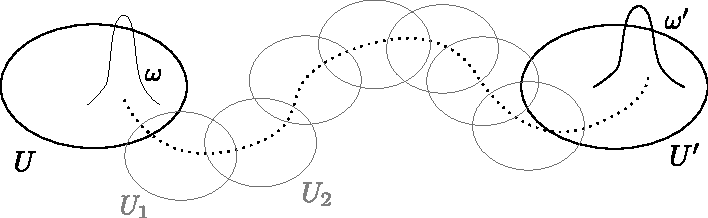
\includegraphics[width=0.8\textwidth]{Images/bumpforms1.pdf}
     \caption{We can cover the path between $U$ and $U'$} \qedhere
\end{figure}
\end{proof}

\begin{lemma} \label{lemmalocfinite}
Every $n$-form on $M$ is cohomologous to a locally finite sum of bump forms.
\end{lemma}
\begin{proof}
Pick a cover $(U_i, \varphi_i), \varphi_i \colon U_i \rightarrow \varphi_i(U_i) \subseteq \rfield^n$, and a locally finite refinement $V_j$ (recall the definition contained in def. \ref{paracompactness}) with a subordinate partition of unity $\lambda_j$ (i.e. $\sum_j \lambda_j = 1$). Then:
\[ \omega = \sum\limits_j (\lambda_j \omega) \sim \sum\limits_{\substack{j \text{ s.t. } \\ \int \lambda_j \omega \not = 0}} \underbrace{\left( \frac{\lambda_j \omega}{\int \lambda_j \omega} \right)}_{\text{bump form}} \cdot \underbrace{\left ( \int \lambda_j \omega \right )}_{\text{coefficients}}  \, .\]
And the sum is locally finite because we chose a locally finite refinement, which is always possible since manifolds are paracompact (thm \ref{paracompactnessthm}).
\end{proof}

\begin{theorem} \label{surjintegral}
If $M$ is a connected, smooth manifold of dimension $n$, such that $\partial M = \emptyset$ and $M$ is oriented, then the map:
\begin{align} \label{surjmap}
H^n(M) &\rightarrow \rfield \\
[\omega] &\mapsto \int_M \omega \nonumber
\end{align}
is well defined and surjective.
\end{theorem}
\begin{proof}
Since $\partial M = \emptyset$, we have $\int_M (\omega + d \eta) = \int_M \omega$ by Stokes's theorem. So, the definition does not depend on the element of the equivalence class chosen. Moreover, let $(U_i, \varphi_i)$  be a chart from the oriented atlas, and let $\omega=f(x_1, \ldots, x_n) dx^1 \wedge \ldots \wedge dx^n$ in $U_i$, with $f$ smooth function, $f > 0$. Then, $\int_M \omega > 0$. Since $\omega$ and $c \, \omega$ are cohomologous $\forall \, c \in \rfield$, we have that for every real number $\lambda$ we can consider a $n$-form $c\,  \omega$ such that $\int_M c\, \omega = \lambda$. So, the map is surjective.
\end{proof}

\begin{definition} \label{closedman}
A manifold $M$ is closed if it is compact and $\partial M = \emptyset$.
\end{definition}

\begin{tcolorbox}
\begin{example}
$S^1$ is a closed manifold. A torus is closed as well.
\end{example}
\end{tcolorbox}

\begin{theorem} \label{1dimthm}
If $M$ is a connected, smooth manifold of dimension $n$, $\dim \left( H^n(M) \right) \le 1$. If $M$ is also closed and oriented, $H^n(M) \cong \rfield$.
\end{theorem}
\begin{proof}
Using the previous theorem \ref{surjintegral}, we just need to verify how many values $\int_U \omega$ can have, where $U$ open subset of $M$ diffeomorphic to $\rfield^n$ (Notice: $\partial U = \emptyset$ because $U$ is open). Now, every element of $H^n(M)$ is cohomologous to a (real) multiple of  a bump form in a fixed chart $(U, \varphi)$. Bump forms have integral $ =\pm 1$. Therefore, the value of the integral of a closed-but-not-exact $n$-form in $H^n(M)$ can be any real number. Since the map \eqref{surjmap} is surjective, we have the first thesis. If $M$ is also closed, then the map \eqref{surjmap} given by integration is also injective. The proof of this is on page 454, \citetalias{Lee}, using that $H^k(M)=H_c^k(M)$ if $M$ is compact.
\end{proof}

\begin{theorem}
Let $M$ be a connected, compact, orientable manifold with $\partial M \not = \emptyset$ and of dimension $n$. Then $H^n(M) = 0$.
\end{theorem}
\begin{proof}
It suffices to find a bump form which is cohomologous to zero in $M$. Once we find it, we have the thesis because $M$ is connected, so any other bump form in the manifold is zero by proposition \ref{prop2bumpforms}. Also, by lemma \ref{lemmalocfinite}, every $n$-form is cohomologous to a locally finite sum of zero-forms, i.e. it is a zero form and we would have the thesis.
\begin{figure}[H] \label{Fig:bumpforms2}
     \centering
     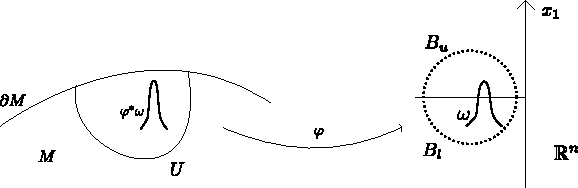
\includegraphics[width=0.8\textwidth]{Images/bumpforms2.pdf}
     \caption{We can find a bump form cohomologous to a zero form}
\end{figure}
Let's find such a bump form. First, let's consider a boundary chart $(U, \varphi), \varphi \colon U \rightarrow \rfield^n \cap \{x_1 < 0\}$ (such that $\varphi(U)$ is a half-ball) and a bump form $\omega$ compactly supported in the interior of the half-ball. We will also consider the other half-ball. We will call $B_l$ the lower half-ball ($B_l = \varphi(U)$) and we will call $B_u$ the other half. We consider another bump form $\omega_u$ contained in $B_u$ such that:
\[ \int_{B_u} \omega_u = \int_{B_l} - \omega \, . \]
It is always possible, because bump forms can only have integral $=\pm 1$.
Now, we consider the form $\omega_u + \omega$ and we extend it by zero. It is compactly supported in the open ball $B \equiv B_u \cup B_l$. By remark \ref{bumpremark} we have that $\omega_u$ and $-\omega$ are cohomologous, so $d\eta = \omega_u + \omega$. Thus:
\[ \restrict{d\eta}{B_l} = \restrict{\omega_u}{B_l} + \restrict{\omega}{B_l} = \restrict{\omega}{B_l} \, . \]
Then, $\varphi^* \eta$ is a primitive of the bump form $\varphi^* \omega$. So, $\varphi^* \omega$ is the zero form we were looking for.
\end{proof}

What if we remove orientation? Recall that we can't compute integrals without orientation.
\begin{theorem}
Let $M$ be a connected but not orientable manifold of dimension $n$. Then: $H^n(M) = 0$.
\end{theorem}
\begin{proof}
Let's cover $M$ by an atlas $(U_i, \varphi_i), \varphi_i \colon U_i \rightarrow \varphi_i(U_i) = \rfield^n$ (we choose the atlas such that $\varphi(U_i) = \rfield^n$). Let's consider an open set $U_0$.
\begin{figure}[H] \label{Fig:bumpforms3}
     \centering
     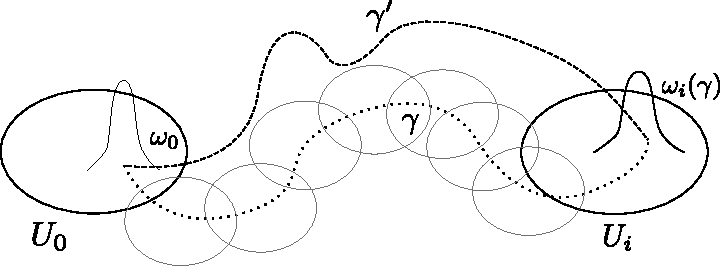
\includegraphics[width=0.8\textwidth]{Images/bumpforms3.pdf}
     \caption{We can consider two paths connecting $U_0$ and $U_i$}
\end{figure}
Let's consider another set $U_i$ from the cover, $U_0 \not = U_i$. Since $M$ is a connected manifold, it is also path-connected, so there exists a path $\gamma \colon [0, 1] \rightarrow M$ that connects $U_0$ to $U_i$. By the same reasoning of the proof of proposition \ref{prop2bumpforms}, we get that a bump form $\omega_0$ contained  in $U_0$ is cohomologous to a bump form $\omega_i(\gamma)$ contained in $U_i$. But, since $M$ is not orientable, there also exists a second path $\gamma'$ connecting $U_0$ and $U_i$, and a second chain of charts covering $\gamma'$, such that, repeating the same procedure, $\omega_0$ is cohomologous to $\omega_{i'}(\gamma')$ with the opposite sign of before (i.e. the integrals have opposite signs). Notice that even if we cannot integrate on $M$, we can integrate on the charts. It means that:
\[ \omega_i(\gamma) \sim \omega_0 \sim \omega_{i'}(\gamma') \sim -\omega_0 \, . \]
So, $\omega \sim - \omega \Leftrightarrow 2 \omega \sim 0$.
\end{proof}

\begin{remarkbox}\begin{remark}
The proofs of the following facts are similar to the previous ones: given a connected manifold $M$:
\begin{itemize}
\item $M$ not compact, $\partial M = \emptyset \Rightarrow H^n(M)=0$,
\item $M$ compact $\Rightarrow H_c^*(M) = H^*(M)$,
\item $M$ not compact, oriented, $\partial M= \emptyset \Rightarrow H^n_c(M)=\rfield$.
\end{itemize}
\end{remark}\end{remarkbox}

\begin{theorem}[Brouwer] \label{brouwerthm}
Let $f \colon \overline{B_1(0)} \rightarrow \overline{B_1(0)} \subset \rfield^n$ be smooth. Then, $f$ has a fixed point, i.e. $\exists \, x \in \overline{B_1(0)}$ such that $f(x)=x$.
\end{theorem}

\begin{proof}
Let's prove it for $f$ smooth. If $f$ is continuous but not smooth, we can approximate it using smooth maps (Weierstrass approximation). Moreover, we will prove it for $n \ge 2$ (for $n=0, 1$ it is a consequence of the intermediate value theorem).
By contradiction: let's assume $f$ has no fixed point. Then we consider the map
\begin{align*}F \colon \overline{B_1(0)} &\rightarrow \partial \overline{B_1(0)} = S^{n-1} \\
x &\mapsto \substack{\text{unique intersection with }S^{n-1} \\ \text{ of the ray passing through }x \text{ and } f(x)}
\end{align*}
$F$ is a smooth function: we will not verify it because it is not interesting for the proof. Moreover, we notice that if $y \in \partial \overline{B_1(0)} \Rightarrow F(y) = y$.
\begin{figure}[H] \label{Fig:ball10}
     \centering
     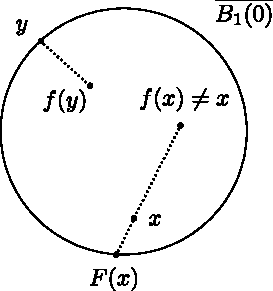
\includegraphics[width=0.3\textwidth]{Images/B_10.pdf}
     \caption{$F$ sends every point of the ball on its border}
\end{figure}
Let's now consider the map: $\iota \colon S^{n-1} \rightarrow \overline{B_1(0)}$ such that $F \circ \iota = \id_{S^{n-1}}$. What happens here? $\iota$ sends any point $z$ on the surface of the ball to the ball itself. $\iota$ is defined in such a way that the position of $\iota(z)$ must be on the line connecting $z$ and $f(\iota(z))$. This way, when we apply $F$ to $\iota(z)$ we go back to $z \in S^{n-1}$. Now, we can consider the pulback:
$$\id_{S^{n-1}}^* = \iota^* \circ F^* \quad \oast$$
where we consider $F^*$ acting on closed-but-not-exact forms: $F^* \colon H^*(S^{n-1}) \rightarrow H^*(\overline{B_1(0)})$. If $* = n-1$, the map:
$$F^* \colon \underbrace{H^{n-1}(S^{n-1})}_{\cong \rfield} \longrightarrow \underbrace{H^{n-1}(\overline{B_1(0)})}_{\cong \,0}$$
has to be injective because of $\oast$ (if the composition of maps is injective, the first map acting is injective). But this is impossible because $H^{n-1}(S^{n-1}) \cong \rfield$ (maybe it was proved in the exercise sheets?) and $H^{n-1}(\overline{B_1(0)}) \cong 0$, with $B_1(0)$ $n$-dimensional ball. In order to prove the latter, we can't use the Poincarè lemma because $\overline{B_1(0)}$ is not homeomorphic to $\rfield^n$ (one is compact and the other is not, and compactness is left invariant under homeomorphisms). But we can prove that $\id \colon \overline{B_1(0)} \rightarrow \overline{B_1(0)}$ is homotopy equivalent to the map $\text{zero} \colon \overline{B_1(0)} \rightarrow \overline{B_1(0)}$ that sends every element of $\overline{B_1(0)}$ to $0 \in \overline{B_1(0)}$. Once we do this, we use the fact that the space itself is homotopy equivalent to the trivial set (for $n \ge 2$) and then the de Rham cohomology must be trivial as well.
\end{proof}

\begin{remarkbox}\begin{remark}
The important assumption of the Brouwer theorem \ref{brouwerthm} is that the entire space is $\overline{B_1(0)}$. We also notice that the theorem can be seen as a corollary of the \href{https://en.wikipedia.org/wiki/Borsuk-Ulam_theorem}{Borsuk-Ulam theorem}. It says that there exists at least a couple of antipodal points on the Earth surface with same temperature and barometric pressure (if we assume temperature and pressure to be two continuous functions).
\end{remark}\end{remarkbox}

\begin{definition}[degree of a map] \label{degreemap}
Let $f \colon M \rightarrow  N$ be smooth, $N, M$ closed manifolds (see def.  \ref{closedman}), orientable and of the same dimension. Then, the degree of $f$ is
\begin{equation}
\deg(f) = \frac{\int_M f^* \omega}{\int_N \omega}, \quad \text{for a form } \omega \in \Omega^n(N) \text{ s.t. } \int_N\omega \not = 0 \, .
\end{equation}
\end{definition}

\begin{remarkbox}\begin{remark}
The definition \ref{degreemap} does not depend on the $\omega$ chosen: if $\omega_1, \omega_2$ are $n$-forms with the same integral, they are cohomologous by the proof of theorem \ref{1dimthm} (the isomorphism is given by integration). Then we can write $\omega_1 = \omega_2 + d\eta$ and we get the same degree by using the naturality of the pullback ($f^* d \eta = d f^* \eta$) and Stokes's theorem. Moreover, the degree of a map is homotopy invariant: if $f_0, f_1 \colon M \rightarrow N$ are two homotopic maps, then $f_0^* = f_1^*$, so $f_0$ and $f_1$ have the same degree.
\end{remark}\end{remarkbox}

\begin{tcolorbox}
\begin{example} \label{degreeexample}
$ $
\begin{itemize}
\item $\deg(\id_M) = 1$,
\item $\deg($constant map$)=0$, because the definition of pullback uses the pushforward: $f^* \omega = \omega (f_*, \ldots)$,
\item If $M, N$ are closed, orientable and of the same dimensions, from the previous two points we know that the identity map cannot be homotopy equivalent to a constant map,
\item If $M=N=S^1$, let's consider
\begin{align*}
f_k \colon S^1 &\rightarrow S^1 \subset \mathbb{C} \\
e^{i \varphi} = z &\mapsto z^k
\end{align*}
Then we have $\deg(f_k) = k$, indeed we can consider $\omega = d\varphi, \varphi$ angular coordinate on $S^1$ (cf. example \ref{angexample}). We stress out that $d\varphi$ is not exact (it is just a bad notation) because $\varphi$ is not a well defined function (it is well defined up to a $2\pi$ angle). Then, we have:
$$\int_{S^1} \omega = 2\pi, \quad \int_{S^1} f_k^* d\varphi = \int_{S^1} k \,d\varphi = 2\pi k \, \Rightarrow \,  \deg(f_k)=k$$
where we used that $\varphi$ is the angular coordinate, so $f(e^{i\varphi}) = e^{i k \varphi}$,
\item For the next theorem, we introduce the concept of critical value and regular value of a function $f$. A critical value is the image of a critical point. A point $p$ is a regular value for $f$ if $D_q f$ is a surjective map for every $q \in f^{-1}(p)$: in a simpler way, $p$ is a regular value if it is not a critical value.
\end{itemize}
\end{example}
\end{tcolorbox}

\begin{theorem}
For all $f \colon M \rightarrow N$, in the hypotheses of def. \ref{degreemap}, the degree of $f$ is an integer. In particular, it is the signed count of preimages of a regular value.
\end{theorem}
\begin{proof}
Let consider a regular value $p\in N$ of $f$. The value $p$ exists thanks to \href{https://en.wikipedia.org/wiki/Sard's_theorem}{Sard's theorem}. Sard's theorem states that the set of the critical values of a smooth function $f$ from a manifold to another one is a null-measure set. We can apply this theorem to our case (and whenever $f$ is not smooth we can approximate it by smooth functions if it is at least continuous). Indeed, if the set of critical values has zero measure, its complementary set (the regular values) has dimension $n$.
In particular, $f^{-1}(p)$ is a submanifold of dimension 0 or, analogously, a submanifold of codimension $n$ (not proved). So, $f^{-1}(p)$ consists of a finite collection of points $q_1, \ldots, q_m$. By the inverse function theorem, there exists a neighbourhood $U_i$ of $q_i \in f^{-1}(p)$ such that $\restrict{f}{U_i}$ is a diffeomorphism onto its image. Let $\omega$ be a bump form supported in $\bigcap_i f(U_i) = V$. Then:
$$\int_M f^* \omega = \sum\limits_i \underbrace{\int_{U_i} f^* \omega}_{\substack{=\pm \int_{f(U_i)} \omega \\ \text{depending} \\ \text{on orientation}}} = \sum\limits_i \left ( \pm \int_V \omega \right )$$
So, the degree is an integer: the signed count of preimages of a regular value. The sign depends on the orientation (i.e. the sign of the determinant of the Jacobian at $p_i, \forall\, i$).
\end{proof}

\section[Poincarè Duality]{\crule[blue!70!white]{0.3cm}{0.4cm}  Poincarè Duality}

In the last section, we studied the degree of a map. It is not always possible to find a map of non-vanishing degree between manifolds of the same dimension. For instance, every smooth map $S^2 \rightarrow T^2 = S^1 \times S^1$ has degree 0.

\begin{tcolorbox}
\begin{example}
Let's consider a smooth map $f \colon S^2 \rightarrow T^2=S^1 \times S^1$.
\begin{minipage}{\textwidth} \label{Fig:torus}
\vspace{1em}
     \centering
     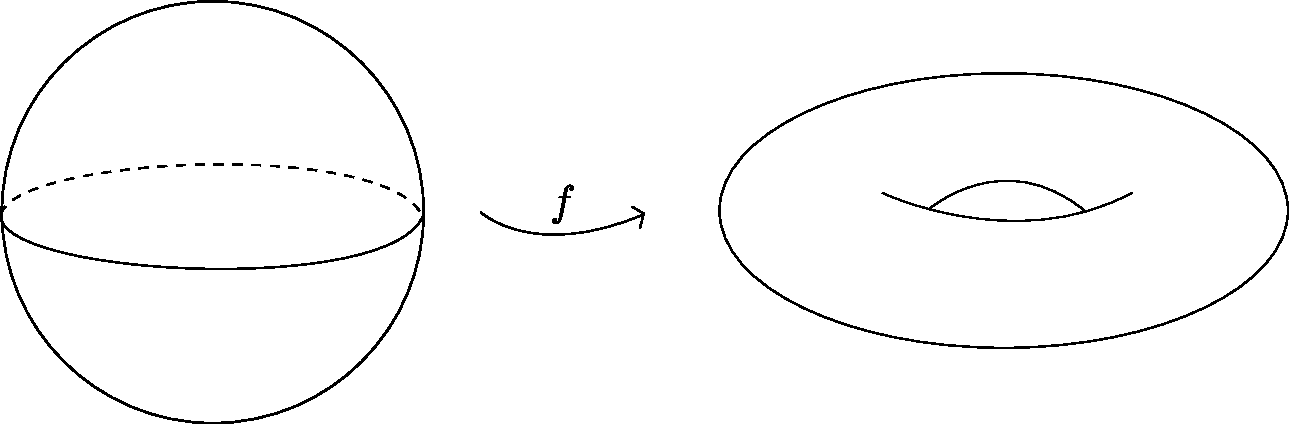
\includegraphics[width=0.6\textwidth]{Images/torus.pdf}
     \captionof{figure}{$f \colon S^2 \rightarrow T^2$}
\end{minipage}
The map $f$ has degree 0, indeed the pullback $f^*\colon H^2(T^2) \rightarrow H^2(S^2)$ is the zero map. In order to show this, we consider two projection maps, $\pr_1$ and $\pr_2$, defined as follows:
\begin{center}
\begin{tikzcd}
                    & T^2=S^1 \times S^1 \arrow[ld, "\text{pr}_1"'] \arrow[rd, "\text{pr}_2"] &                     \\
{(S^1, d\varphi_1)} &                                                                         & {(S^1, d\varphi_2)}
\end{tikzcd}
\end{center}
where  $\varphi_i$ are angular functions and $d\varphi_1$ and $d\varphi_2$ are not exact, as already seen in the example \ref{degreeexample}.
We choose $\omega \equiv (\pr_1^* d \varphi_1) \wedge (\pr_2^* d\varphi_2)$. We have:
$$\int_{S^1 \times S^1} \omega = \int_{S^1} d\varphi_1 \int_{S^1} d\varphi_2 = 4 \pi^2$$
Now, we have:
$$f^* \omega = \underbrace{\left ( (\pr_1 \circ f)^* d \varphi_1 \right )}_{\text{closed 1-form on }S^2} \wedge \underbrace{\left( \pr_2 \circ f)^* d \varphi_2 \right)}_{\text{also closed}}$$
 because we used the proposition \ref{pullbackprop}, point 3, and because of the naturality of the pullback. Now, $H^1(S^2)=0$ (not proved, but it can be computed using the Mayer-Vietoris theorem \ref{mvthm}). So, every closed form on $S^2$ is exact. Thus, the two closed 1-forms above are actually exact forms.
So, $(\pr_1\circ f)^*d\varphi_1 = d g$ and we have that
$$f^*\omega = dg \wedge \left( (\pr_2 \circ f)^* d \varphi_2 \right)$$ is exact because the product between an exact form  and a closed one is an exact form. Finally:
$$\int_{S^2} f^* \omega = 0$$
using Stokes's theorem (we get $\int_{B^3} 0=0$).
\end{example}
\end{tcolorbox}

\begin{theorem}
Let $M$ be a closed, oriented, connected $n$-dimensional manifold. Then, if we consider maps to $S^n$, not only the degree is homotopy invariant but the converse is also true:
\begin{equation}
f_0 \sim f_1 \colon M \rightarrow S^n \Leftrightarrow \deg(f_0) = \deg(f_1)
\end{equation}
\end{theorem}

\begin{theorem}[Poincarè Duality]
Let $M$ be an oriented, connected, $n$-dimensional manifold with $\partial M = \emptyset$. We define the map:
\begin{align}
\text{PD} \colon H^k(M) \times H^{n-k}_c (M) &\rightarrow \rfield \\
([\omega], [\eta]) &\mapsto \int_M (\omega \wedge \eta) \nonumber
\end{align}
where $[\omega]$ and $[\eta]$ are equivalence classes for different equivalence relations. This map is non-degenerate\footnote{PD is non-degenerate: if $[\omega]$ is non-zero, we can find a $[\eta]$ such that PD$([\omega], [\eta]) \not = 0$.} and establishes a natural isomorphism:
\begin{align}
H^k(M) &\cong (H^{n-k}_c(M))^* \\
(H^k(M))^* &\cong H_c^{n-k}(M)
\end{align}
Moreover, if $M$ is closed, then $H^k(M) \cong (H^{n-k}(M))^*$ and these vector spaces have finite dimension.
\end{theorem}
\begin{proof}[Idea of the proof]
The proof is not hard, but it is quite long, under the assumption that exists a finite "good" cover by charts. Here, "good" means that any non-empty intersection of charts is diffeomorphic to a ball. Then, the proof is by induction on the cardinality of a finite good cover. Then, we also need to use the zig-zag lemma for $H^*$ and $H^*_c$ and the so-called 5-lemma.
\end{proof}

\section[Riemannian Metric and the Hodge-$\star$ Operator]{\crule[red!60!white]{0.3cm}{0.4cm}  Riemannian Metric and the Hodge-$\star$ Operator}
\begin{definition}[Riemannian metric] \label{riemmetric}
Let $M$ be a smooth manifold. A Riemannian metric is a map
\begin{equation}
g \colon \restrict{(TM \times TM)}{\Delta} \rightarrow \rfield
\end{equation}
fiberwise bilinear, symmetric and positive definite. Here, $\Delta=\{(x, x) \, | \, x \in M\} \subset M \times M$ is the diagonal set\footnote{$\Delta$ is a submanifold of $M \times M$ and it is diffeomorphic to $M$.} of $M$.
\end{definition}

\begin{remarkbox}\begin{remark}
Let's analyze the definition \ref{riemmetric}. The term "fiber" denotes the preimage of a point. The restriction of the metric $g$ to $\Delta$ means that the first and the second arguments of the map $g$ are in the same space $T_x M$, for some $x \in M$. Moreover, we can generalize the definition to consider metrics with the same hypotheses, but which are not positive definite and non-degenerate: this how a Lorentzian metric is defined.
\end{remark}\end{remarkbox}

\begin{theorem}
Every smooth manifold admits a Riemannian metric,
\end{theorem}
\begin{proof}
Let's cover $M$ with charts $(U_i, \varphi_i)$ and pick a subordinate partition of unity $\phi_j \colon V_j \subset U_{i(\ldots)}\rightarrow \rfield$. We can do that because our manifold is second-countable and paracompact (the latter one is actually a necessary hypothesis). On each set $V_j$ there is a metric $g_j$ coming from the coordinates. Then, $g = \sum\limits_j \lambda_j g_j$ is a Riemannian metric (easy to verify). The key point is that a convex combination of positive definite is still positive definite).
\end{proof}

\begin{remarkbox}\begin{remark}[Counter-example for Lorentzian metric]
It is not true that every manifold admits a Lorentzian metric. For instance, $S^{2n}$ does not.
\end{remark}\end{remarkbox}

A Riemannian metric assigns lengths to vectors, angles between vectors...we want to extend this (or, analogously, a Lorentzian metric) to alternating forms.
\newline
\begin{remarkbox}
%[label=genmetricremark]
 \begin{remark} \label{genmetricremark}
A Riemannian metric provides an isomorphism:
\begin{align*}
\musFlat \colon T_p M &\rightarrow (T_p M)^* \\
v &\mapsto (\omega \mapsto g(v, w)) \, .
\end{align*}
And the inverse is the map $\musSharp \equiv \musFlat^{-1}$. This is called musical isomorphism and it is related to the action of "raising and index" and "lowering an index" in physics. For more info, see page 342 of \citetalias{Lee}. Such a map can be extended as $\musFlat \colon TM \rightarrow T^*M$ and so associate a 1-form to each vector field (since vector fields are sections of the tangent bundle and 1-forms are sections of the cotangent bundle). We can then further extend the isomorphism to alternating forms:  there exists a canonical isomorphism:
\begin{align*}
\text{Alt}^k(T_p^*M) & \overset{\sim}{\longrightarrow} (\text{Alt}^k(T_p M))^* \, . 
\end{align*}
It lets us define a Lorentzian metric on forms (in particular, to extend it from $T_p^* M$ to $\Lambda^kT_p^* M \equiv \text{Alt}^k (T_p^* M)$). A precise definition is the following one: if $e_1, \ldots, e_n$ is an orthonormal basis of $T_pM$ and $\delta^1, \ldots, \delta^n$ is the dual basis, then:
\begin{equation*}
\langle \delta^{\mu_1} \wedge \ldots \wedge \delta^{\mu_k}, \delta^{\lambda_1}\wedge \ldots \wedge \delta^{\lambda_k} \rangle = \begin{cases*}
0, & if $(\lambda_1, \ldots, \lambda_k) \not = (\mu_1, \ldots, \mu_k)$\\
\varepsilon_{\lambda_1}\cdots \varepsilon_{\lambda_k}, &if $(\lambda_1, \ldots, \lambda_k) = (\mu_1, \ldots, \mu_k)$
\end{cases*}
\end{equation*}
where: $g(\cdot, \cdot) = \langle\cdot, \cdot\rangle$ is the Lorentzian/Riemannian metric defined on forms, $\mu_1 < \ldots < \mu_k$, $\lambda_1 < \ldots < \lambda_k$, and $\varepsilon_{\lambda_i}= \langle e_i, e_i \rangle = \pm1$ (we always have the "$+$" sign for the Riemannian metric, whereas we have some "$-$" sign for a Lorentzian metric). Thus, $\langle \cdot, \cdot \rangle$ for alternating forms is symmetric.
\end{remark} \end{remarkbox}

\begin{definition}[Volume form]
If $M$ is an oriented manifold, then a volume form $\omega$ on $T_pM$ is a  differential $n$-form such that:
\begin{equation}
\omega(e_1, \ldots, e_n) = 1, \quad \forall\, \{e_1, \ldots, e_n\} \text{ orthonormal basis of }T_pM
\end{equation}
\end{definition}

\begin{remarkbox}\begin{remark} \label{diffbasisrem}
If $e_1', \ldots, e_n'$ is another oriented orthonormal basis, then $\exists$ a $f$ such that:
\begin{align*}
f \colon T_pM &\rightarrow T_p M \\
e_i &\mapsto e_i'
\end{align*}
is a linear map, orthogonal and positive definite (i.e. $\det f = 1$). Moreover:
$$\omega(e_1', \ldots, e_n') = \omega(f(e_1), \ldots, f(e_n))  = (\det f) \omega(e_1, \ldots, e_n) =1$$
where we used the alternating property of forms:
\[ \omega (T e_1, \ldots, T e_n) = (\det T) \omega(e_1, \ldots, e_n) \] when $T$ is a linear map (see page 354 of \citetalias{Lee} for more details).
\end{remark}\end{remarkbox}
We saw how a volume form reacts to an orthonormal basis. How about a general basis?

\begin{lemma}
Let $f_1, \ldots f_n$ be an oriented basis (not orthonormal) of $T_p M$. Let $\omega$ be a volume form. Then:
\begin{equation}
\omega(f_1, \ldots, f_n)=\sqrt{\det g_{ij}}, \qquad g_{ij} \equiv \langle f_i, f_j \rangle  \, .
\end{equation}
\end{lemma}
\begin{proof}
Let $e_1, \ldots, e_n$ be an oriented orthonormal basis and let's consider the map:
\begin{align*}
F \colon T_pM &\rightarrow T_p M \\
e_i &\mapsto f_i
\end{align*}
which has positive determinant. With respect to the basis $e_1, \ldots, e_n$, $F$ is represented by the matrix $A=(\alpha_{ij})$, where $\alpha_{ij}$ such that $f_i = \sum \alpha_{ij} e_j$. Now,
$$\langle f_i, f_j \rangle = \left \langle \sum\limits_l \alpha_{il} e_l, \sum\limits_m \alpha_{jm}e_m \right \rangle = \ldots= \sum\limits_l \alpha_{il}\alpha_{jl} = \left( A^t A \right )_{ij} \, .$$
Thus,
\begin{align*}
\omega(f_1, \ldots, f_n) &= \omega(F(e_1), \ldots, F(e_n)) = (F^* \omega)(e_1, \ldots, e_n)= \det A \, \omega(e_1, \ldots, e_n) =\\
&= \det A = \sqrt{\det g_{ij}} \, .
\end{align*}
where we used again the definition of pullback for linear maps (see remark \ref{diffbasisrem}), the formula $\det(A A^t) = \det(A)^2$, and the fact that $\omega$ is a volume form.
\end{proof}

\begin{lemma}[Hodge-$\star$ operator]
Let $V$ be an oriented\footnote{In 3 dimensions, a vector space is "right-oriented" if its basis is oriented according to the right hand. In general dimension there is not such a thing as a preferred orientation. In this case we just want to say that we arbitrarily chose an orientation for our basis.} $\rfield$-(vector space), $\dim V =n$. Let $\langle \cdot, \cdot \rangle$ be a non-degenerate, symmetric bilinear form. Let $\omega$ be the canonical volume form. Then there is a unique linear map
\begin{equation}
\star \colon \Lambda^k V^* \rightarrow \Lambda^{n-k}V^* , \qquad \forall\, k=0, 1, \ldots, n
\end{equation}
such that:
$$\langle \eta, \zeta \rangle \omega = \eta \wedge \star \zeta, \qquad \forall \, \eta, \zeta \in \Lambda^k V^* \, .$$
The map $\star$ is the Hodge-$\star$ (Hodge star) operator.
\end{lemma}
\begin{proof} $ $
\begin{description}
\item[Uniqueness:] Assume $\star, \tilde{\star}$ satisfy the assumption. Then:
$$\underbrace{\eta}_{\in \Lambda^k V^*} \wedge \underbrace{(\star \zeta - \tilde{\star} \zeta)}_{\Lambda^{n-k} V^*} = 0, \qquad \forall\, \eta, \zeta \in \Lambda^k V^* \, .$$
If $\star \not = \tilde{\star} \Rightarrow \exists \, \zeta : \, \forall\, \eta, \, \eta \wedge \underbrace{(\star \zeta- \tilde{\star} \zeta)}_{\not = 0} = 0$, but it is easy to find an $\eta$ violating this equality, writing $\star \zeta - \tilde{\star} \zeta \in \Lambda^{n-k} V^*$ in terms of a basis.
\item[Existence:]   To prove existence, we use an orthonormal basis  $e_1, \ldots, e_n$ of $V$ and the dual basis $\delta^1, \ldots, \delta^n$ of $V^*$. Recall that for $1 \le \mu_1 < \ldots < \mu_k \le n, 1 \le \lambda_1 < \ldots < \lambda_k \le n$, we have (see also remark \ref{genmetricremark}):
$$\oast = \langle \delta^{\lambda_1} \wedge \ldots \wedge \delta^{\lambda_k}, \delta^{\mu_1} \wedge \ldots \wedge \delta^{\mu_k} \rangle \omega = \begin{cases*}
\varepsilon_{\mu_1}\cdots \varepsilon_{\mu_k} \omega, &if $(\lambda_1, \ldots, \lambda_k) = (\mu_1, \ldots, \mu_k)$ \\
0, &otherwise
\end{cases*}$$
And in order to have the thesis, we need:
$$\oast \overset{!}{=} \delta^{\lambda_1} \wedge \ldots \wedge \delta^{\lambda_k} \wedge \star (\delta^{\mu_1} \wedge \ldots \wedge \delta^{\mu_k})$$
where the symbol $\overset{!}{=}$ means "must be equal", as usual. It follows that $\star (\delta^{\mu_1} \wedge \ldots \wedge \delta^{\mu_k})$ is a multiple of $\delta^{\nu_1} \wedge \ldots \wedge \delta^{\nu_{n-k}}$, where $\nu_1, \ldots, \nu_{n-k}$ such that $\{\mu_1, \ldots, \mu_k, \nu_1, \ldots, \nu_{n-k}\} = \{1, \ldots, n\}$ (because we want to get a multiple of $\omega$). More precisely, using the permutations, only one coefficient of $\star (\delta^{\mu_1} \wedge \ldots \wedge \delta^{\mu_k})$ is non-zero, and it is the one for $(\lambda_1, \ldots, \lambda_k) = (\mu_1, \ldots, \mu_k)$:
$$\star(\delta^{\mu_1} \wedge \ldots \wedge \delta^{\mu_k}) = \varepsilon_{\mu_1} \cdots \varepsilon_{\mu_k} \sgn  \left (
\begin{matrix}
1 \ldots k &k+1 \ldots n \\
\mu_1 \ldots \mu_k &\nu_1 \ldots \nu_{n-k}
\end{matrix} \right )
\delta^{\nu_1} \wedge \ldots \wedge \delta^{\nu_{n-k}}
$$
This holds without any assumption on the order of the $\lambda_i$, and it defines $\star$ on a basis. The resulting operator has the desired property:
\[ \langle \eta, \zeta \rangle \omega = \eta \wedge \star \zeta, \qquad \forall\, \eta, \zeta \in \Lambda^kV^* \, .  \qedhere \]
\end{description}
\end{proof}

\begin{remarkbox}\begin{remark}[Properties of $\star$]
The Hodge-$\star$ operator has the property:
\begin{equation} \label{starprop}
\star \star = \varepsilon_1 \cdots \varepsilon_n (-1)^{k(n-k)}, \quad \text{on } \Lambda^k V^*
\end{equation}
where $\varepsilon_i = \langle e_i, e_i \rangle = \pm 1$, so $\Index(V) \equiv \varepsilon_1 \cdots \varepsilon_n$ is the number of "$-$" signs that we get. Let's prove the property \eqref{starprop} on a basis:
\begin{align*}
& \star \star (\delta^{\mu_1} \wedge \ldots \wedge \delta^{\mu_k}) = \star \left ( \varepsilon_{\mu_1} \cdots \varepsilon_{\mu_k} \sgn \left(
\begin{matrix}
1\ldots k &k+1\ldots n \\
\mu_1\ldots \mu_k & \nu_1 \ldots \nu_{n-k}
\end{matrix}
\right)  \delta^{\nu_1} \wedge \ldots \wedge \delta^{\nu_{n-k}}\right) = \\
&= \underbrace{\varepsilon_{\mu_1} \cdots \varepsilon_{\mu_k} \varepsilon_{\nu_1} \cdots \varepsilon_{\nu_k}}_{=(-1)^{\Index}} \sgn \underbrace{ \left(
\begin{matrix}
1\ldots k &k+1\ldots n \\
\mu_1\ldots \mu_k & \nu_1 \ldots \nu_{n-k}
\end{matrix}
\right)}_{\tau} \sgn \underbrace{ \left(
\begin{matrix}
1\ldots n-k &n-k+1\ldots n \\
\nu_1 \ldots \nu_{n-k}& \mu_1 \ldots \mu_{k}
\end{matrix}
\right)}_{\sigma} \\
& \delta^{\mu_1} \wedge \ldots \wedge \delta^{\mu_k} \overset{(1)}{=}  \varepsilon_1 \ldots \varepsilon_n \sgn (\tau) \sgn(\sigma^{-1}) \delta^{\mu_1} \wedge \ldots \wedge \delta^{\mu_k} = \\
&=  \varepsilon_1 \ldots \varepsilon_n \sgn \underbrace{ \left (
\begin{matrix}
1 \ldots k & k+1 \ldots k+n-k \\
k -n+1 \ldots n & \ \ldots n-k
\end{matrix} \right)
}_{\sigma^{-1} \circ \tau} \delta^{\mu_1} \wedge \ldots \wedge \delta^{\mu_k}  = \\
&= \varepsilon_1 \ldots \varepsilon_n (-1)^{k(n-k)} \delta^{\mu_1} \wedge \ldots \wedge \delta^{\mu_k}
\end{align*}
where we used: (1) $\sgn(\sigma^{-1}) = \sgn(\sigma)$. So, up to a sign, $\star \star$ is an involution. Moreover, up to a sign, $\star$ is an isometry. Indeed:
$$\star \eta \wedge \star \star \zeta = \langle \star \eta , \star \zeta \rangle \omega = (-1)^{\Index V} \langle \eta, \zeta \rangle \omega \, .$$
\end{remark}\end{remarkbox}

\begin{lemma}
Given a symmetric, bilinear, non-degenerate pairing $\langle\cdot, \cdot \rangle$ on a manifold $M$ (oriented, smooth, compact), there is a induced non-degenerate, symmetric, bilinear pairing
\begin{align}
\Omega^k(M) \times \Omega^k(M) &\rightarrow \rfield \\
(\eta, \zeta) &\mapsto \int_M\langle \eta, \zeta \rangle \omega = \int_M (\eta \wedge \star \zeta) \equiv \langle \eta, \zeta \rangle_M \nonumber
\end{align}
 \end{lemma}

\begin{definition} [Codifferential]
The map $\delta = (-1)^k \star d \star^{-1} \colon \Omega^{n-k}(M) \rightarrow \Omega^{n-k-1}(M)$ is called codifferential (it decreases the degree of a form).
\end{definition}

\begin{remarkbox}\begin{remark}
We notice that $\delta^2 = 0$. Moreover, we want to compare $\star \delta $ and $d \star$. So, let $\zeta \in \Omega^{k+1}(M)$, we compute the following:
\begin{align*}
\overbrace{d \underbrace{\star\, \zeta}_{n-k-1}}^{n-k} &\overset{\eqref{starprop}}{=} (-1)^{k(n-k) + \Index(M)} \star \star d \star \zeta \overset{(1)}{=} (-1)^{k(n-k) + \Index(M)} \star \star d \star \star \underbrace{\star^{-1} \zeta}_{n-(k+1)} \overset{\eqref{starprop}}{=} \\
&=(-1)^{k(n-k) + 2\Index(M) + (n-k-1)(k+1)} \star \star d \star^{-1} \zeta = \ldots = (-1)^k \star \delta \zeta
\end{align*}
where we used: (1) $1=\star \star^{-1}$.
\end{remark}\end{remarkbox}

\begin{lemma} The following holds:
\begin{equation}
d(\eta \wedge \star \zeta) = (d\eta) \wedge \star \zeta + (-1)^{\deg \eta} \eta \wedge d \star \zeta = \ldots = d \eta \wedge \star \zeta + \eta \wedge \star \delta \zeta
\end{equation}
where $\eta \in \Omega^k(M), \zeta \in \Omega^{k+1}(M)$. If $M$ is closed, then:
\begin{equation}
0 = \int_M d(\eta \wedge \star \zeta) = \langle d \eta, \zeta \rangle_M + \langle \eta, \delta \zeta \rangle_M \, .
\end{equation}
Using the notations of mathematical analysis (where an operator $A^*$ is the adjoint of $A$ if $\langle A^*x,  y \rangle = \langle x, Ay \rangle, \forall\, x, y  $ in the domain of $A$ and $A^*$), we say that $-\delta$ is formally the adjoint of $d$.
\end{lemma}

\begin{remarkbox}\begin{remark}[Notation]
We will write:
$$d_k \colon \Omega^k(M) \rightarrow \Omega^{k+1}(M)$$
$$\delta_k \colon \Omega^{n-k}(M) \rightarrow \Omega^{n-k-1} (M)$$
\textbf{Notice that} in the first part of the course the first map above was called $d_{k+1}$ and not $d_k$! We are changing notation here with respect to the notations used in the course.
Then:
$$(-1)^k \delta_k \star = \star \delta_k$$
and $-\delta_k$ is the formal adjoint of $d_{n-k-1}$ (via $\langle \cdot, \cdot \rangle_M$).  In addition, $(-1)^k \delta_k$ is conjugate to $d_k$ (via $\star$).
Let's look again at the adjointness condition:
\begin{equation} \label{adjcondition}
\oast \quad \langle d_k \eta, \zeta \rangle _m + \langle \eta, \delta_{n-k-1} \zeta \rangle _M = 0 \, .
\end{equation}
\textbf{Fact}: From $\oast$, it follows that $\ker d_k \subset (\im \delta_{n-k-1})^{\bot}$. Actually, also $\supset$ holds. Furthermore: $\ker \delta_{n-k} = (\im d_{k-1})^{\bot}$.
For finite-dimensional vector spaces, this would imply:
\begin{equation}
\ocdot \quad \Omega^k(M) = (\ker d_k) \oplus (\im \delta_{n-k-1}) = (\ker \delta_{n-k}) \oplus (\im d_{k-1})
\end{equation}
Actually, $\ocdot$ holds also for infinite-dimensional spaces, thanks to the following theorem.
\end{remark}\end{remarkbox}

\begin{theorem}[Fundamental theorem of Hodge-de Rham theory]
The expression $\ocdot$ above is an orthogonal direct sum decomposition.
\end{theorem}

\begin{corollary} The following holds:
\begin{align}
\ker d_k &= \Omega^k(M) \cap \ker d_k = \left ( \ker (\delta_{n-k} \oplus \im(d_{k-1}) \right ) \cap \ker d_k = \\
&= \left ( (\ker \delta_{n-k}) \cap \ker d_k \right) \oplus \im d_{k-1} \, . \nonumber
\end{align}
Comparing first and last term, and remembering that the de Rham cohomology of $M$ is $H^{k}(M) = \faktor{\ker d_k}{\im d_{k-1}}$, we have that $H^{k}(M) \cong \left ( (\ker \delta_{n-k}) \cap \ker d_k \right)$. In a similar way:
\begin{equation}
\ker \delta_{n-k} = \im \delta_{n-k-1} \oplus \left ( \ker d_k \cap \ker \delta _{n-k} \right ) \, .
\end{equation}
\end{corollary}

\begin{lemma}[Harmonic forms]
Elements of $\mathcal{H}^k(M) \equiv \ker d_k \cap \ker \delta_{n-k}$ are closed and coclosed (i.e. closed with respect to $\delta$), and they are said to be harmonic. The Laplace operator is $\Delta = d \circ \delta + \delta \circ d$, and
\begin{equation} \label{deltaeqn}
\mathcal{H}^k(M) = \ker \left ( \restrict{\Delta}{\Omega^k(M)} \right ) \, .
\end{equation}
\end{lemma}
\begin{proof}[Proof of \ref{deltaeqn}]
$\eta, \zeta \in \Omega^k(M)$.
\begin{description}
\item["$\subseteq$":] trivial by definition of $\Delta$,
\item["$\supseteq$":]  We have:
$$0 = \langle \Delta \eta, \zeta \rangle_M = \langle d \circ \delta \eta + \delta \circ d \eta, \zeta \rangle_M =- \langle d \eta, d \zeta \rangle_M - \langle \delta \eta, \delta \zeta \rangle_M, \quad \forall\, \zeta \, .$$
where we used the adjointness \eqref{adjcondition}. Since it holds for every $\zeta$, it is also true for $\zeta = \eta$:
$$0 = - \underbrace{|| d \eta ||^2}_{\ge 0} - \underbrace{||\delta \eta||^2}_{\ge 0}$$
and the equality holds $\Leftrightarrow \eta \in \ker d_k, \eta \in \ker \delta_{n-k}$.\qedhere
\end{description}
\end{proof}

\begin{corollary}[Hodge theorem] There is an isomorphism
\begin{equation}
\mathcal{H}^k(M) \rightarrow H^k(M) \, .
\end{equation}
Moreover, we have:
\begin{center}
\begin{tikzcd}
\mathcal{H}^k(M) \arrow[r] \arrow[d, "\star^{-1}"', shift right] & H^k(M) \arrow[d, shift right]                        \\
\mathcal{H}^{n-k}(M) \arrow[u, "\star"', shift right] \arrow[r]  & H^{n-k}(M) \arrow[u, "\sim \text{PD}"', shift right]
\end{tikzcd}
\end{center}
\end{corollary}

\begin{remarkbox}\begin{remark}
$ $\newline
\textbf{Fact}: $\mathcal{H}^k(M)$ has finite dimension ($\Delta$ is an elliptic operator).

\textbf{Fact} (Hodge decomposition):
$$\Omega^k(M) = \mathcal{H}^k(M) \oplus d_{k-1} \Omega^{k-1}(M) \oplus \delta_{n-k-1} \Omega^{k+1}$$
is an orthogonal sum decomposition.
\end{remark} \end{remarkbox}

%Add picture vector field pag. 207 Lee, and pag. 221. CHECK from page 14

\clearpage
\fancyhf{}
\begin{thebibliography}{AA}
\addcontentsline{toc}{section}{Bibliography}
\bibitem{Lee}
J. M. Lee, Introduction to Smooth Manifolds, 2nd edition, Springer
\bibitem{Notes}
\href{https://www.physik.uni-muenchen.de/lehre/vorlesungen/wise_19_20/Differentiable-Manifolds/material/skript-TMP.pdf}{Lecture notes} Differentiable Manifolds Sachs, Vogel WS 19
\end{thebibliography}


\end{document}
